% REMEMBER: You must not plagiarise anything in your report. Be extremely careful.
\documentclass{l4proj}

%==================================================================================================s
% Put any additional packages here
% You can add any packages you want, as long as it does not alter the overall format (e.g. don't change the margins or the reference style).
%
\usepackage{pdfpages} % if you want to include a PDF for an ethics checklist, for example
\usepackage{enumitem}
\usepackage{hyperref}
\usepackage{float}
\usepackage{physics, amssymb, graphicx, fancyvrb}
\usepackage{multirow, siunitx}

\definecolor{forestgreen}{RGB}{1, 140, 65}
\definecolor{brickred}{RGB}{173, 2, 2}
\definecolor{golden}{RGB}{207, 159, 4}


\begin{document}

%==================================================================================================
%% METADATA
\title{Automatic Illustration of Text via Multimodal Interaction}
\author{Stergious Aji (2546916A)}
\date{\today}

\maketitle

%==================================================================================================
%% ABSTRACT
\begin{abstract}
    Automatic videography systems pose a serious challenge for effective performance evaluations. Often, this is limited to qualitative assessments with capricious human participants leading to biased and non-reproducible results. To address this issue, this paper proposes a two-part system. The first part is a new autonomous videography tool that leverages multimodal representations of both images and text to automatically illustrate spoken language in audio sources. The second half involves a novel ground-truth construction interface intended to streamline the creation of test collections for the quantitative evaluations of automatic videography systems. This interface intends to solve the challenge of evaluating videography tools by allowing the swift calculation of standard Information Retrieval metrics such as Average Precision and Recall. Importantly, these metrics permit fair comparisons with alternate systems, which was previously infeasible with subjective user evaluations. The final implemented system successfully produced a user-friendly interface that eases relevance assessment effort. Experiments also demonstrate that the new system enhances many aspects of the preceding videography system.

    % Every abstract follows a similar pattern. Motivate; set aims; describe work; explain results.
    % \vskip 0.5em
    % ``XYZ is bad. This project investigated ABC to determine if it was better. 
    % ABC used XXX and YYY to implement ZZZ. This is particularly interesting as XXX and YYY have
    % never been used together. It was found that  
    % ABC was 20\% better than XYZ, though it caused rabies in half of subjects.''
\end{abstract}

%==================================================================================================
%% ACKNOWLEDGEMENTS
% \chapter*{Acknowledgements}
% Enter any acknowledgements here. This is optional; you may leave this blank if you wish, or remove the entire chapter
%
% We give thanks to the Gods of LaTeX, who in their eternal graciousness, have granted that this document may compile without errors or overfull hboxes.

%==================================================================================================
% EDUCATION REUSE CONSENT FORM
% If you consent to your project being shown to future students for educational purposes then insert your name and the date below to  sign the education use form that appears in the front of the document. You must explicitly give consent if you wish to do so.
% If you sign, your project may be included in the Hall of Fame if it scores particularly highly.
%
% Please note that you are under no obligation to sign this declaration, but doing so would help future students.

\def\consentname {Stergious Aji} % your full name
\def\consentdate {\today} % the date you agree
\educationalconsent


%==================================================================================================
\tableofcontents
%==================================================================================================
%% Notes on formatting
%==================================================================================================
% The first page, abstract and table of contents are numbered using Roman numerals and are not included in the page count. 
%
% From now on pages are numbered using Arabic numerals. Therefore, immediately after the first call to \chapter we need the call \pagenumbering{arabic} and this should be called once only in the document. 
%
%
% The first Chapter should then be on page 1. 

% PAGE LIMITS
% You are allowed 40 pages for a 40 credit project and 30 pages for a 20 credit report. This includes everything numbered in Arabic numerals (excluding front matter) up to but *excluding the appendices and bibliography*.
%
% FORMATTING
% You must not alter text size (it is currently 10pt) or alter margins or spacing. Do not alter the bibliography style. 
%
%==================================================================================================
%
% IMPORTANT
% The chapter headings and structure here are **suggestions**. You don't have to follow this model if it doesn't fit your project. Every project should have an introduction and conclusion, however.  If in doubt, your supervisor can give you specific guidance; their view takes precedence over the structure suggested here.
%
%==================================================================================================
\chapter{Introduction}
% reset page numbering. Don't remove this!
\pagenumbering{arabic} 

% Why should the reader care about what are you doing and what are you actually doing?
This chapter serves to outline the motivations for creating an automatic videography tool, as well as the rationale for a subsequent interface for annotating ground-truth, specifically using multimodal representations of images and text. 

% \textbf{Motivate} first, then state the general problem clearly. 
\section{Motivations}
\subsection{Automatic Videography of Audio}
Text-to-image retrieval is a topic that has gained increased interest in recent years since the advent of new deep-learning approaches that have outperformed prior work \citep{gordo2017end}. These advancements have illuminated new innovations in a number of areas, particularly automatic content creation \citep{singer2022make}. Furthermore, the rise in video production \citep{tprisevideo} has also demanded a drive for more automated systems, especially in the realm of music. However, on popular platforms such as \cite{youtube}, music often lacks any accompanying video content which can be detrimental to its overall prosperity. This can be due to various reasons such as a lack of funding, resources, or song popularity. More commonly, this issue arises from music tracks that were originally recorded in analogue formats which have since been digitised for upload to the platform.

Moreover, the proposed tool has applications beyond music tracks, as it can effectively enhance educational materials and podcasts. According to the study by \cite{benefits_of_mmv}, participants who viewed video lectures consisting of both visual and auditory content performed better on the post-exam than those who watched lectures with only one of those elements. As a result, incorporating multiple modes of information such as visual, audio, and textual, can increase the accessibility of the subject and improve user retention. In addition, this could help cater to diverse learning styles such as those identified in Fleming's VARK acronym \citep{vark}.

One of the main motivations of this project is to build on and enhance previous work on the Automatic Videography of Audio Tracks of Songs by \cite{parker}. Parker's thesis achieved a functioning video generation tool for audio tracks sourced from YouTube. However, the system suffered from a number of drawbacks that we seek to address with this project. A more in-depth review of the thesis is conducted in Section \ref{sec:background_parker} of the Background.

\subsection{Ground-Truth Annotation Interface}
With an evergrowing supply of automatic videography systems, it is important to assess and contrast their respective capabilities. Nevertheless, we have found that there is a lack of objective procedures for evaluating comparative performances between videography systems, particularly in terms of measuring their accuracy at image retrieval from text. Image relevance can and has been assessed with qualitative user surveys but this can often be very subjective and sensitive to personal preferences and present moods \citep{mohammadi2014subjective}. More importantly, if the objective is to compare against the outcomes of a previously evaluated system, additional user studies must be carried out using the same demographic of individuals to evaluate new systems \citep{voorhees2005trec}. Not only is this approach impractical and time-consuming, but it also leads to results that are unrepeatable and biased.

This can be mitigated if instead, a set of true labels are annotated in advance for provided audio sources which can then be used to evaluate multiple videography systems on those same audio sources. It is vital that a static image collection is used for ground-truth constructing and evaluating in order for the production of repeatable and standardised performance metrics.

This called for a user-friendly interface to assess the relevance of images from the textual content present in given audio sources. Under the hood, this ground-truth constructor interface can theoretically use the same pipeline as the automated videography system that we are already creating. 


\section{Aims}
This project aims to produce a piece of software that can take any audio source and automatically generate a video from it. The video will consist of time-aligned imagery corresponding to the spoken words in the audio. In addition, this software will include a novel annotation interface for assessing image relevance from text prompts. This will let the user construct a set of ground-truths for each portion of the supplied audio source. This will be achieved by letting the annotator select the set of images that they perceive as the most fitting to the text or song lyric in a given chunk of audio. This set of images will be picked from a top-$k$ list retrieved by our system.

Since there is a high priority for precise ground-truth construction, the software must be intuitive to use with clear instructions for the assessor to follow. It is imperative, therefore, that we strive to develop a platform with a user-friendly interface that is widely accessible. Additionally, since the aim is for anyone to use this application, appropriate error handling must be in place to accommodate users from a broad range of technical backgrounds. We also aspire to make our system modular in design. This way, more technical users would be able to swap in any image collection with minimal configuring if required.

At the end of this project, we endeavour to provide a set of completed ground-truth for a pre-defined list of audio sources using our annotation interface. This data will be made available in an accessible format so that it can be used to measure the quality of existing and future videography systems using standard Information Retrieval (IR) metrics like Average Precision (AP), F-Measure, and Normalised Discounted Cumulative Gain (nDCG).

Finally, as stated in our motivations, we wish to fix the limitations of the previous video generation system as well as extend its functionality. Our objective is to expand the application of the tool to any audio source, rather than restricting it to the YouTube platform. This also means, our tool must be able to support the transcription of multiple languages and accents. Finally, we intend to tackle the image retrieval process using a different approach that introduces semantics in order to retrieve more relevant images.

% However, the data will not be restricted to the task of automatic videography, due to it simply consisting of a set of relevance assessments of images from text. Hence, the data can be used in existing or new text-to-image research in general. A recent example of such a possible use case is investigating the effeciveness of Variable Depth Pooling (CITE), more details are discussed in the Background section \ref{sec:background_pooling}.

% In order to justify creating a novel annotation interface, we must first explore existing solutions and their corresponding strengths and limitations.


%==================================================================================================
\chapter{Background}
This chapter serves to lay the foundations in order to contextualise this project within the field of Information Retrieval (IR). Firstly, a look into the origins of the field, specifically image retrieval, will be conducted. This will be followed by a discussion of the recent advancements in computer vision to allow multimodal representations of images with natural language. We will briefly look into the history of relevance assessment to ground our problem of evaluating IR systems and justify our proposed approach. Next, the previous thesis on automatic videography will be critiqued, with the aim of identifying its merits and shortcomings. This will form the basis upon which our project will build. Finally, an outline of what current solutions exist to solve our problem of assessing the relevance of images from text queries will be provided.

\section{The History of Image Retrieval}
Image retrieval is an important branch within the field of IR which has evolved over the past several decades. Recent years have witnessed an exponentially growing collection of images, spanning various domains such as academia, medicine, social media, and the military. This makes it all the more important that efficient mechanisms are in place to scour these databases. The earliest such mechanisms can be traced back to the 1970s. Known plainly as Text-Based Image Retrieval (TBIR) systems, they relied on keyword-based querying of a relational database \citep{chang1979tbir}. Consequently, every image in the database had to be labelled with appropriate keywords and a description. This was a popular framework at the time, but with the exponential growth of datasets, manual annotation became infeasible. Moreover, the results were often of low quality due to the limited ability of the systems to accurately interpret the user's intent; not to mention, the subjectivity of human perception during annotation.

Fortunately, researchers at the time also began looking into the application of computer vision to solve the task. The key idea involved extracting visual features from the images like colour, texture, and shape and utilising these to index them into the database. This made it possible to use images as the search criteria in order to find images with similar features \citep{chang1981pictorial}. This approach later became known as Content-Based Image Retrieval (CBIR) as better image processing techniques emerged in the 1990s allowing easier extraction of features. Furthermore, as the capability to extract additional visual characteristics improved, images started being represented in increasingly higher dimensions \citep{zheng2017sift}. This often led to data sparsity problems in which the movement into higher dimensions caused similar data points to drift apart as the volume of the space grew too quickly for the data to keep up. A well-known phenomenon coined as the \emph{"curse of dimensionality"} \citep{bellman1957dp}.

In the 2000s, researchers developed more sophisticated approaches for text-to-image retrieval, incorporating techniques from natural language processing (NLP) and computer vision. This led to the development of more advanced retrieval models that could accurately match textual queries with semantically relevant images. Some notable works in this period include the Language of Pictures system by \cite{lavrenko2003lop}, the Cross-Media Relevance Models (CMRM) by \cite{rasiwasia2010cmmr}, and the Text-Guided Attention Model (TGAM) by \cite{gao2018tgam}.

The field of image retrieval underwent a significant revolution in the late 2010s with the emergence of deep learning-based approaches. These models are trained using large datasets of text and images and can learn complex semantic representations that capture the meaning of both the textual queries and the visual content of the images. Some notable works in this period include the Deep Visual-Semantic Alignment (DVSA) model by \cite{karpathy2015dvsa} and the Neural Image Caption (NIC) model by \cite{vinyals2015nic}. This even spawned new areas of research with the concept of image synthesis using AI as seen in the StackGAN model by \cite{zhang2017stackgan}. This brings us to the latest developments with OpenAI and CLIP.


\subsection{CLIP: Transforming the Future of Text-to-Image Retrieval}
\label{sec:background_clip}
The year 2021 marked the release of OpenAI's Contrastive Language-Image Pre-Training (CLIP) model and paper \citep{radford2021clip}. This is an effective image-text embedding model based on a transformer architecture. Transformers are a type of deep neural network that was first introduced in a seminal paper by \cite{vaswani2017attention}. They were originally developed for natural language processing tasks leading to several state-of-the-art, pre-trained systems like BERT \citep{devlin2018bert} and GPT \citep{radford2018gpt}. However, it has since been adapted to other domains, most notably computer vision \citep{dosovitskiy2020vit}. These advancements laid the crucial groundwork for the emergence of CLIP.

The CLIP model uses a transformer architecture that is similar to the one used to create the GPT-2 language model \citep{radford2019gpt2}. The model consists of a stack of transformer encoder layers, each of which consists of a self-attention mechanism followed by a feedforward network. The self-attention mechanism allows the model to attend to different parts of the input sequence and learn relationships between them, while the feedforward network applies non-linear transformations to the input features. The transformer encoder layers are used to process both the text and image inputs, allowing the model to learn a multimodal representation that captures the relationship between them. The text input is tokenized using a byte-pair encoding (BPE) scheme, and the resulting tokens are embedded into a high-dimensional vector space. Similarly, the image input is processed by a series of convolutional layers, followed by a global average pooling layer that produces a feature vector that is in the same vector space as the text.

The joint text-image representation is learned by attending to both the text and image features using the self-attention mechanism in the transformer layers. The model is trained to predict whether a given image and text pair belong together, using a contrastive loss function that encourages similar pairs to be closer in the representation space than dissimilar ones. This training objective allows the model to learn a rich representation of both text and images, which can be used for a wide range of downstream tasks. This flexibility is what makes CLIP more appealing than previous models.

The CLIP model was trained on a dataset of over 400 million images and their associated text descriptions. It achieved state-of-the-art performance on a variety of image classification benchmarks, including ImageNet, COCO, and CIFAR-100. One of the key advantages of the CLIP model is its ability to generalise to new tasks and domains without requiring further training. For example, the authors found that the model was able to perform well on a variety of tasks, such as zero-shot classification, image retrieval, and visual reasoning, without any additional fine-tuning. CLIP achieved an impressive top-1 accuracy of 76.3\% on the ImageNet zero-shot benchmark, where the goal is to classify images into novel categories, unseen during training. A significant improvement on the previous state-of-the-art which achieved 11.5\% accuracy.

Overall, the results demonstrate that the CLIP model is capable of learning a rich and flexible representation of both text and images, which allows it to perform well on a broad range of tasks, specifically text-to-image retrieval. The model also has strong generalisation capabilities, which makes it well-suited for applications where data is often scarce or noisy. This makes CLIP an attractive choice for a restrictive project such as this one.


\section{Relevance Assessment}
One of the main objectives of this project is to develop an interface to construct a set of known relevant images from text queries. However, this concept of relevance assessment has a deep history involving a variety of viable strategies so this must be investigated in order to find one most suited to achieving our goal.

Relevance assessment is an integral aspect of IR systems that determines the relevance of documents to a user's query. These documents, while most commonly associated with textual data, can encompass various other forms of data including but not limited to images, videos, and music. In IR, relevance refers to the degree to which a document satisfies a user's information need. Relevance assessment is essential in evaluating IR systems as it ensures that the search engine retrieves only the most pertinent documents and presents them to the user in an appropriate order.

\subsection{Origins}
The concept can be traced back to the early days of IR amidst the rapid expansion of computerised catalogues for military, governmental, and educational purposes in the 1950s. With many different classification and indexing strategies emerging, it became increasingly unclear which was the most effective. This was until the Cranfield experiments conducted by \cite{cleverdon1967cranfield} at Cranfield University, England. These experiments pioneered one of the most widely used evaluation frameworks within IR including fundamental techniques such as query formulation and evaluation metrics. One of the key innovations within the Cranfield paradigm was the development of the relevance assessment methodology. This was the idea of using a fixed test collection of queries designed to represent a wide range of information needs, and manually assessed relevant documents for each query. This test collection is then used to evaluate the effectiveness of different IR systems in retrieving those relevant documents. The experiments also introduced the first IR evaluation metrics, including precision and recall, which are still widely used today. 

During the early days of IR, it was common to use binary relevance assessments, a simple indication of whether a document is relevant or not to a particular query. In the 1970s, researchers explored the use of graded relevance assessments, which allow assessors to assign scores to documents based on their degree of relevance to a query \citep{salton1971smart, robertson1976relvance}. While this method provides a more informative evaluation measure, it greatly increases annotation effort and the subjectivity of judgment.

\subsection{Techniques}
Various techniques have been proposed for performing relevance assessments, including manual assessments, crowdsourcing, and automated techniques:
\begin{itemize}
    \item Manual assessments involve human assessors who painstakingly look at every document and assign relevance scores based on predefined criteria and queries. This is a very time-consuming and expensive process, often requiring expert assessors with specialised knowledge to be able to judge documents accurately. 

    \item Crowdsourcing, on the other hand, involves an open call for a large group of people to assess documents \citep{samimi2014creation}. This can be effective, in generating extensive test collections especially when the documents do not belong to a specific domain of expertise. It also captures a wider range of viewpoints as it brings in assessors from diverse backgrounds. Contrastingly, this can equally bring in bias depending on the assessors' incentives and personal preferences. Finally, this technique makes quality control especially difficult, leading to the potential for fraudulent assessments.
    
    \item More recently, machine learning approaches are being used to predict the relevance of documents based on their content and other features \citep{cao2007ltr}. This technique is much faster and more scalable compared to manual annotation, producing more consistent results across multiple evaluations. However, this technique often lacks the flexibility to adapt to changing evaluation criteria or different types of data. Furthermore, such a system still needs human validation to ensure its predictions are accurate, often leading to a more semi-automated approach.
\end{itemize}

While many more techniques have been developed, manual assessment is still the gold standard in IR evaluation. However, with the exponentially growing size of document collections in the modern day, it is infeasible for humans to judge every document in the corpus for each query. Therefore, strategies such as \textbf{pooling} and \textbf{active learning} \citep{rahman2020testal}, are utilised in order to reduce annotation effort.

\subsection{Depth-Pooling}
\label{sec:background_pooling}
Pooling is a popular strategy used for very large-scale collections of documents, in order to optimise the relevance assessment process. It involves creating a pool of the top-$k$ documents, for a particular query, retrieved from a number of different retrieval systems. The key idea here is that this $k$, which is commonly kept at a constant depth for each query, is much smaller than the size of the corpus. This means that the assessors must only judge the relevance of this modest subset of documents while all the others can be labelled as non-relevant. Trying to further optimise the pooling strategy itself is an evolving area of research. Papers such as \cite{arampatzis2009stop} and \cite{lien2019assumption} propose ways for determining the optimal cut-off point for the number of ranked documents that would satisfy a user's information need by examining the statistics of score distributions.

% (VARIABLE DEPTH POOLING)
% This paper proposes an alternate strategy to pooling, where instead of setting a constant depth, $k$, it should be dependant on the specific query. The rationale behind this central idea is that the number of relevant documents is unlikely to be equal for every query. Some queries are prone to having fewer relevant items in the collection, while others a larger number. The authors hypothesise that this strategy could minimise relevance annotation effort compared to the conventional pooling policy.

\subsection{Active Learning}
Active learning (AL) involves a machine learning approach to iteratively optimise its retrievals by posing queries to a human. These queries are typically in the form of unlabelled data which the human can annotate. The learner can then use this knowledge to find the user's specific information need \citep{burr2012al}. While this approach can be effective in identifying relevant documents, we believe it is not suited for our task. AL is more appropriate for sophisticated supervised learning tasks in which acquiring labelled instances is costly, such as specialised information extraction or speech recognition. In our case, a simple binary relevance assessment will suffice.


\section{Prior Work on Multimodal Assessment}
Before starting to build our system, it is important to look at similar existing solutions to our problem. This section will start off with a deep dive into the previous thesis in order to identify which parts of it we want to build on. Following this, we will focus on the novel annotation interface that we plan to develop by looking at two solutions that could solve a similar problem to the one described in this project. By analysing the design and workflow structure that these solutions employ, we can gather ideas and paint a clearer picture of the interface we want to develop. From the research done here, it was evident that most annotation software provide a wide range of different functionality and tools. While this is certainly a positive in giving users as much freedom as possible, it can equally be a drawback. In most scenarios, users want to focus on a single task, and therefore attempting to learn and navigate a large versatile application can be confusing and a waste of time and resources.

The two relevance assessment software we chose to look at are \textbf{\cite{labelbox}} and \textbf{\cite{superannotate}}. Both pieces of software are similar in aspect to the annotation tool proposed in this project. However, they each have advantages and limitations which further motivate the requirement for our application.

\subsection{Automatic Videography of Audio Tracks of Songs}
\label{sec:background_parker}
\cite{parker} supplied an automatic videography system that generated videos for music tracks sourced from YouTube videos. The project aimed at providing a tool to ease music video creation and investigate the effects of using multimodal information in enriching songs.

\subsubsection{Achievements}
The project achieved a simple web interface, shown in Figure \ref{fig:parker_interface}, where users can supply a YouTube video URL, the artist name and song title as well as the alignment method. On submission, the system will download the video and subsequently isolate the audio and video content. The next steps will depend on the chosen alignment method, so each will be explained one by one. There are three alignment methods available:
\begin{itemize}
    \item \textbf{Forced Alignment:} This method uses a forced alignment model in order to synchronise the retrieved lyrics of the song to the extracted audio. The lyrics are retrieved from the \cite{genius} database using the supplied song title and artist. A word-level dictionary of timings is returned which is used to place relevant imagery at the correct timestamps during video compilation.

    \item \textbf{Lyrical Analysis:} This method only functions for music lyric videos since it works by extracting textual information from the frames of the video using an Optical Character Recognition (OCR) tool. This technique produces phrase-level timings.

    \item \textbf{Caption Extraction:} This method extracts the caption information from the YouTube video directly providing phrase-level alignment information. However, the feasibility of this method hinges on the availability of the captions.
\end{itemize}

The system scrapes the relevant images from Google Images. However, for this approach to work best, images should be searched by keywords. This requires extracting at most two keywords for each segment within the transcript, which this project accomplishes by leveraging YAKE!: Yet Another Keyword Extractor \citep{campos2020yake}. Finally, the alignment information and scraped images are used to compile the final video which is presented to the user.

\begin{figure}[H]
    \centering
    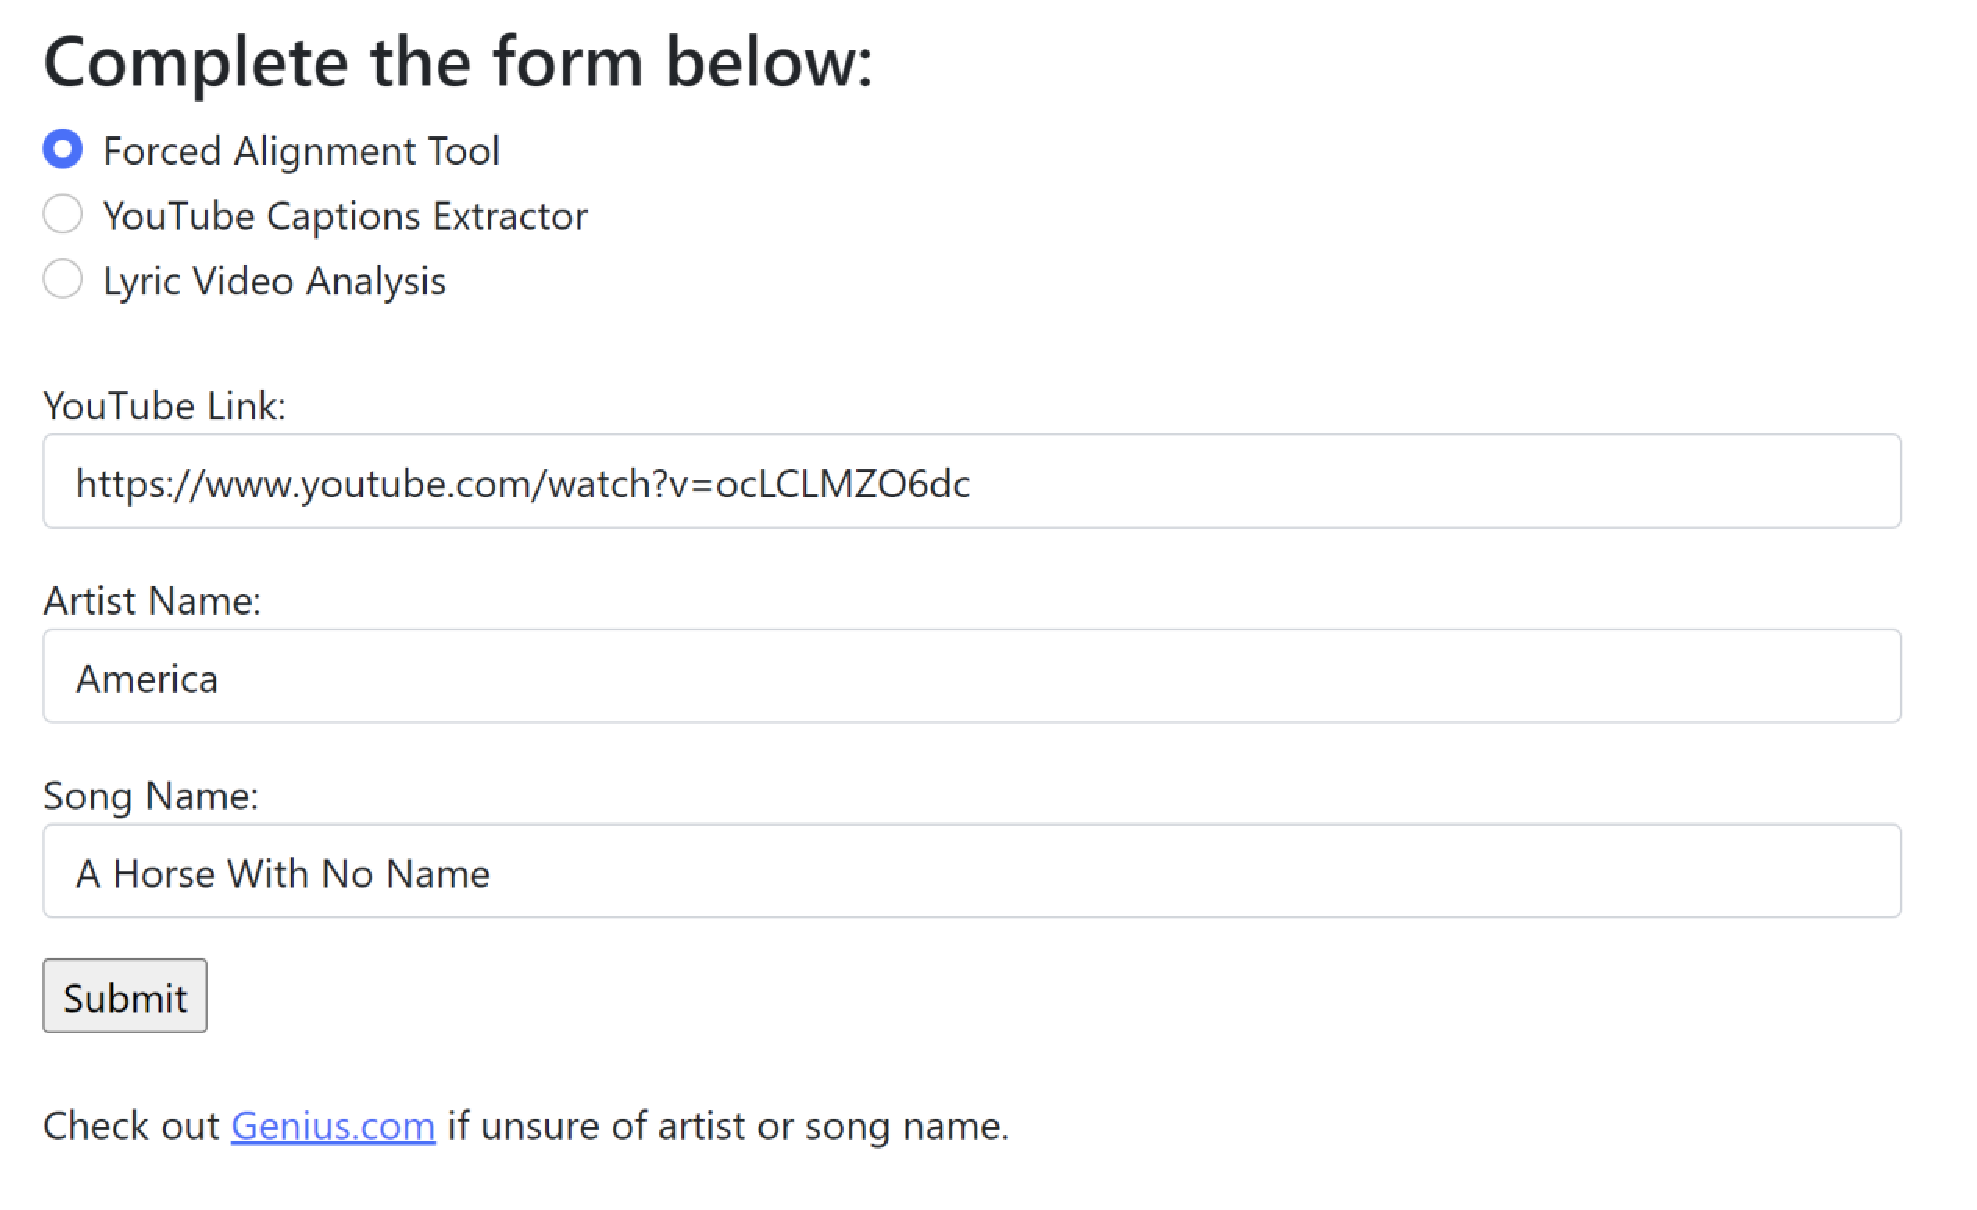
\includegraphics[width=0.8\textwidth]{figures/parker_interface.pdf}
    \caption{An example of using the user interface from the preceding system}
    \label{fig:parker_interface}
\end{figure}

\subsubsection{Problems}
Parker's system made many achievements in generating complementary videos for audio tracks. However, it was restricted to the YouTube platform and emerged with a number of unforeseen drawbacks.

\label{par:metadata_problem}
To begin with, the metadata of YouTube videos was deemed unreliable in procuring the artist's name and the song title. Therefore, the system resorts to obtaining this information from user input. However, this can be problematic since it requires the user to undertake additional research and accurately type the information, which can be prone to errors. 

The prior system was also heavily reliant on several Application Programming Interfaces (APIs) such as YAKE! for keyword extraction, pytesseract \citep{pytesseract} for OCR of frames, and Google Images for scraping images just to name a few. This places a high dependency on these APIs which may not be consistently maintained or may cause version conflicts with other packages. In fact, the AutoLyrixAlign API \citep{gupta2020ala}, utilised for the Forced Alignment approach has since been deprecated at the time of writing.

Additionally, the system suffered from recurring instances of irrelevant images being retrieved. This can be attributed to the disregard of the semantic context of the keywords during the search process. Furthermore, keywords with multiple meanings in the English language often yielded incorrect images.

The ultimate problem identified, which directly prompted our idea of ground-truth construction, stemmed from the evaluation phase of the project. The user surveys exhibited a mixed, albeit predominantly favorable assessment of the system. Nevertheless, the significant variance in ratings and responses to the open-ended questions emphasised the arduousness of conducting qualitative evaluations on automated videography systems. Furthermore, such evaluations produced non-repeatable outcomes.

\subsubsection{Improvements}
Now that the main problems have been identified, we must present solutions so that we can gather the appropriate requirements for this project. The first goal is to generalise the system to any type of audio instead of being restricted to English source material. Adding support for multiple languages would further our goal of increased user accessibility to content. Moreover, this would allow easier content creation for many resource-poor languages.

First of all, let us tackle the metadata problem. We want to avoid relying on the user for metadata information for the audio source which means we must acquire this from somewhere else. This data was primarily used to query the \cite{genius} database in order to retrieve the lyrics transcription for songs so this data is not required for non-musical sources. Therefore, in order to identify the song title and artist, we could use the audio itself as the query. Shazam \citep{wang2006shazam} is an application that can recognise music and movies by listening to a short sample of the audio. It does this by attempting to match the audio's time-frequency signature to one stored in its large catalogue of audio fingerprints to get the correct track information. While this approach would mean an additional API, its benefits of increased automation outweigh the drawbacks.

In order to retrieve more relevant images, it is clear that semantics must be introduced instead of relying on keyword-based searching. Upon researching the recent advancements with CLIP (\ref{sec:background_clip}), we believe this is a viable solution that can mitigate the number of non-relevant images being retrieved. Additionally, the quality and video generation time must be improved when moving forward with this project.

Lastly, we believe our novel ground-truth annotation interface will address the difficulty of evaluating current and future automatic videography systems. The constructed relevance assessments allow for the application of the Cranfield paradigm and computing standard IR metrics. These quantitative measures permit impartial performance comparisons between different systems. More importantly, the experiments can be conducted rapidly and repeatedly without concerns about result consistency.

\subsection{Labelbox}
\label{sec:labelbox}
Labelbox is a cloud-based platform for data labeling and annotation. It is used by many companies to build and improve machine learning models. Founded in 2018, it offers a range of annotation tools including image classification, object detection, and segmentation. Its image classification tool allows users to label images with relevant tags or categories, such as "dog" or "cat". For our specific task, Labelbox allows users to query for specific concepts using natural language, which returns a ranked list of relevant images. The user can then select the most appropriate images by checking a box and saving them for export. An example of this process can be seen in Figure \ref{fig:labelbox_interface}, where an annotator marks relevant images for the concept, \emph{"painting of cocktails"}.

\begin{figure}[h]
    \centering
    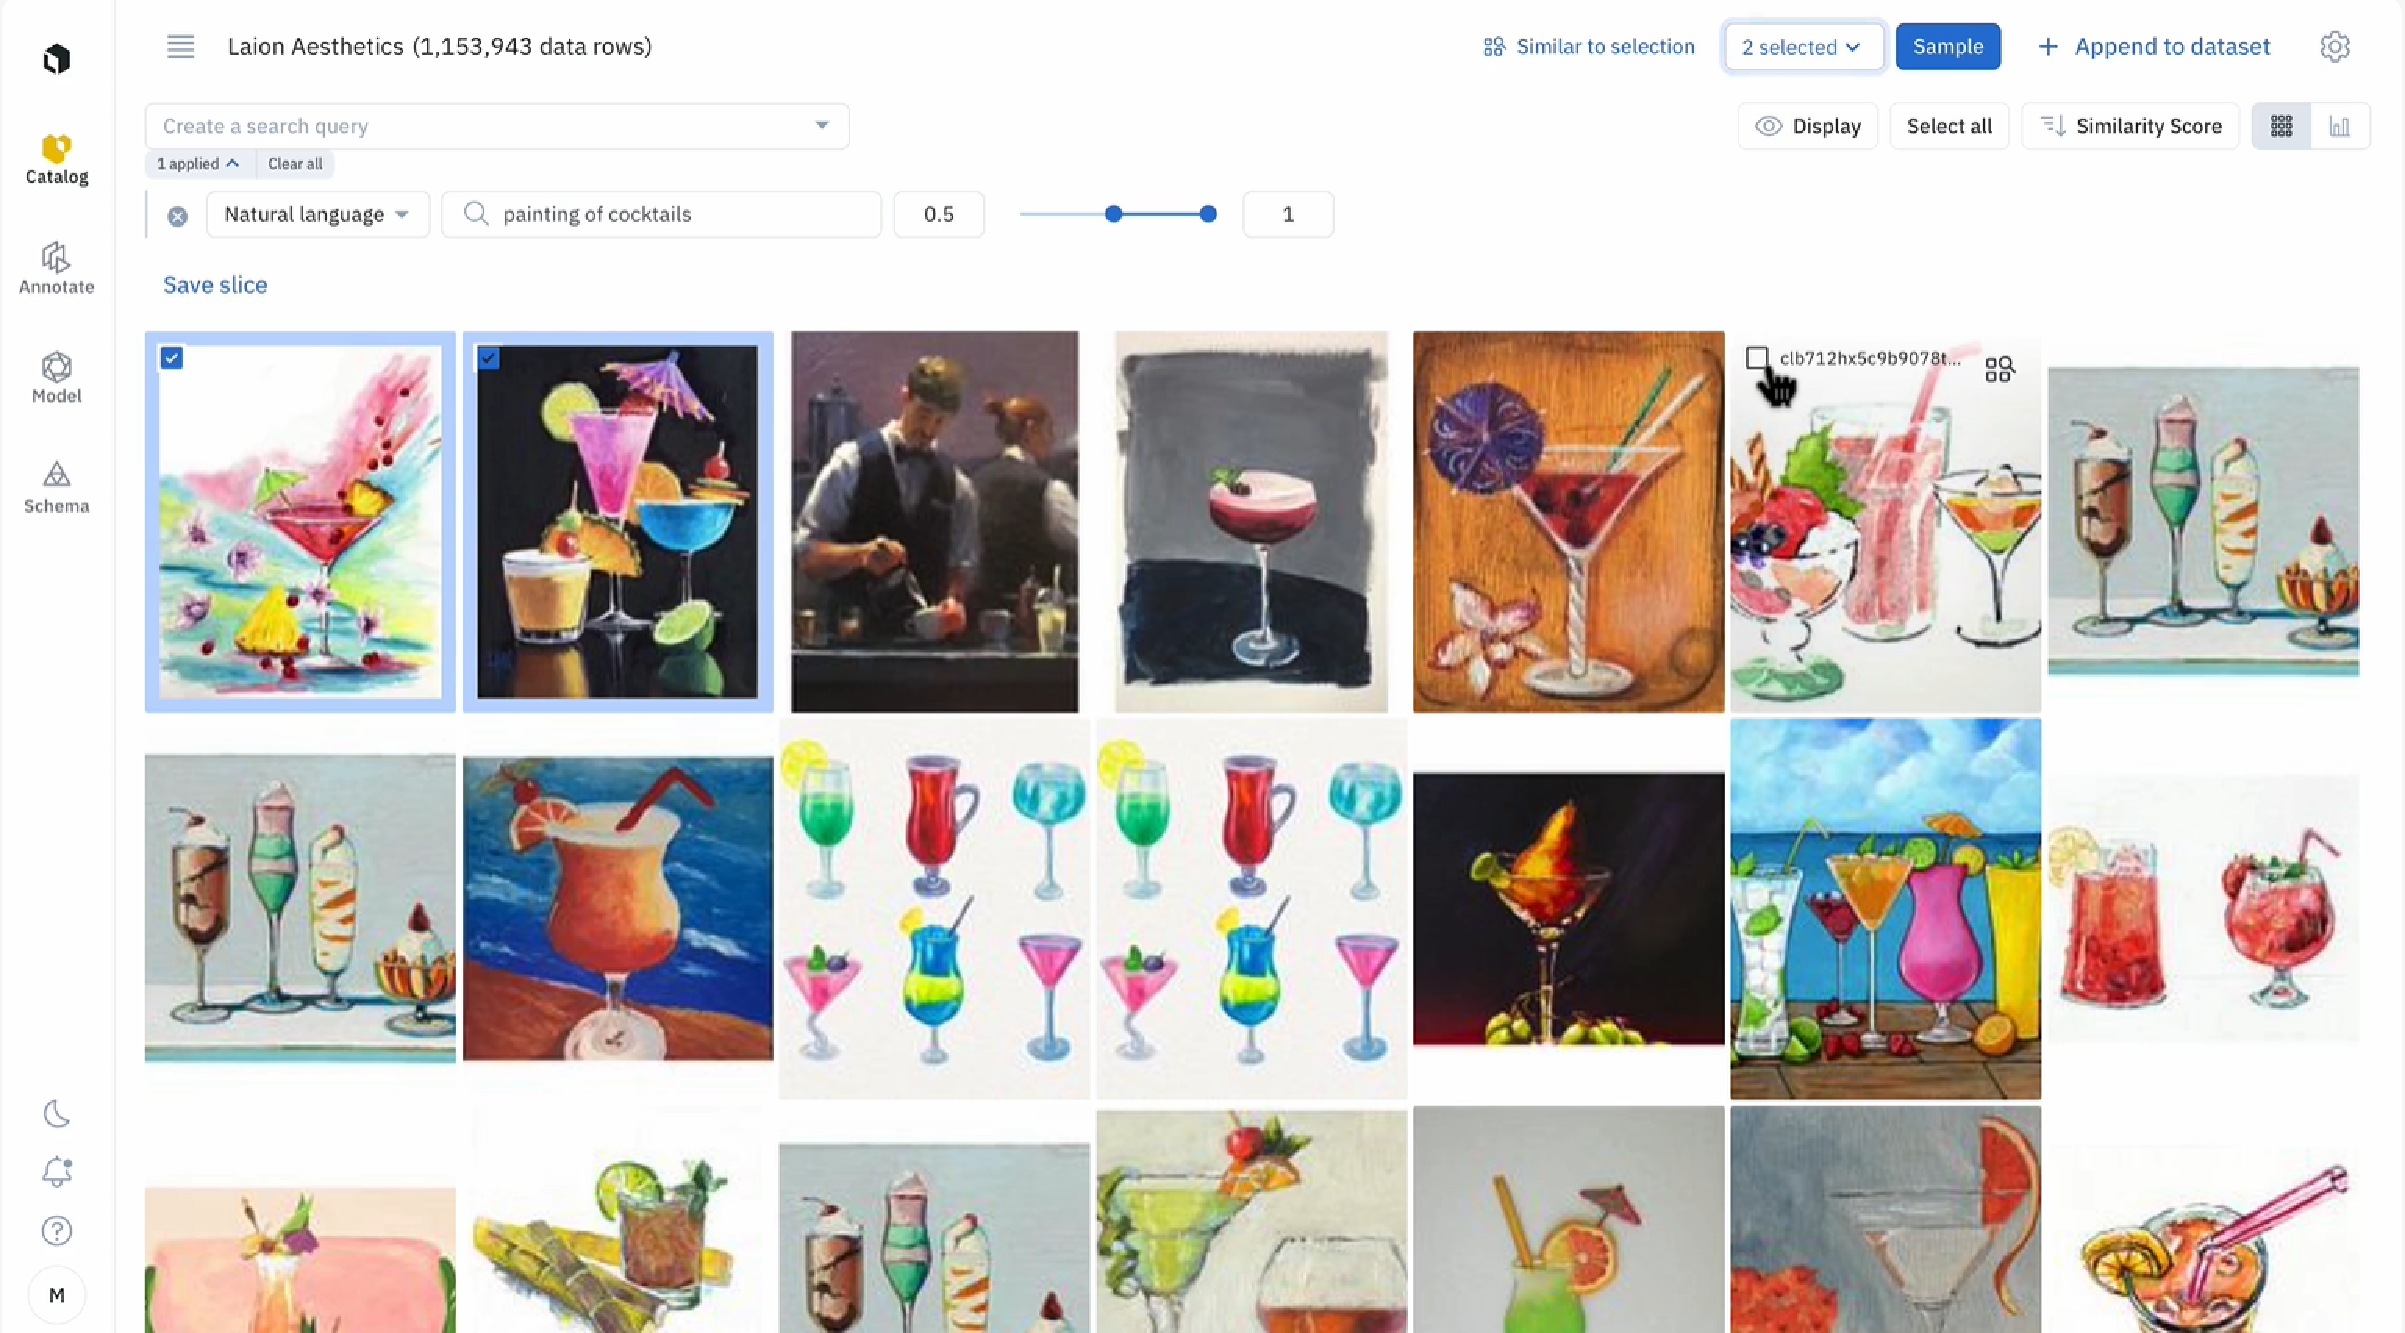
\includegraphics[width=0.95\textwidth]{figures/labelbox_interface.pdf}
    \caption{Relevance assessment of the concept "painting of cocktails" using the Labelbox interface}
    \label{fig:labelbox_interface}
\end{figure}

One of the most appealing features that Labelbox offers is allowing users to customise the embedding model for similarity searching and its aesthetic hyperparameter, as illustrated in Figure \ref{fig:labelbox_model}. Currently, Labelbox only supports the CLIP ViT-B/32 model for images. However, the platform is designed to be compatible with any model, which can be configured using their well-documented API.

\begin{figure}[h]
    \centering
    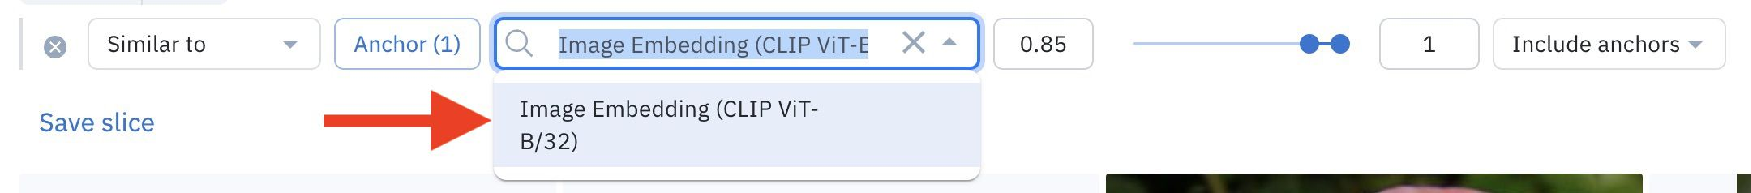
\includegraphics[width=1\textwidth]{figures/labelbox_model.pdf}
    \caption{Labelbox providing the option to customise the image-text embedding model}
    \label{fig:labelbox_model}
\end{figure}

The platform also integrates with popular machine learning frameworks and cloud services, allowing companies to streamline their data labeling workflows and accelerate model development. Despite the platform's slick design, getting acquainted with the application takes time, just due to the sheer multitude of available features and tools.


\subsection{SuperAnnotate}
\label{sec:superannotate}
Founded in 2017, SuperAnnotate is another cloud-based platform for computer vision and machine learning, designed to help users create high-quality image datasets for training and testing models. The platform allows the annotation of images with bounding boxes, polygons, or keypoints, among others, as well as the ability to collaborate with other annotators on the fly. The platform has since grown rapidly and has been used by companies and researchers across diverse industries including autonomous vehicles, medical imaging, and agriculture.

SuperAnnotate is not just restricted to images, it also offers tools for annotating audio, video, LiDAR, and any custom data formats like PDFs or HTML. However, the platform's comprehensive feature set is only accessible via a paid subscription model, which may not be ideal for individuals who require a single tool such as image relevance assessing. Figure \ref{fig:superannotate_interface} depicts SuperAnnotate's interface to query images using natural language, similar to Labelbox (\ref{sec:labelbox}). The interface also allows placing tags in order to filter the retrieved images by specific attributes such as traffic lights that only show red. However, unlike Labelbox, SuperAnnotate does not provide an off-the-shelf embedding model, necessitating users to feed a model themselves.

\begin{figure}[h]
    \centering
    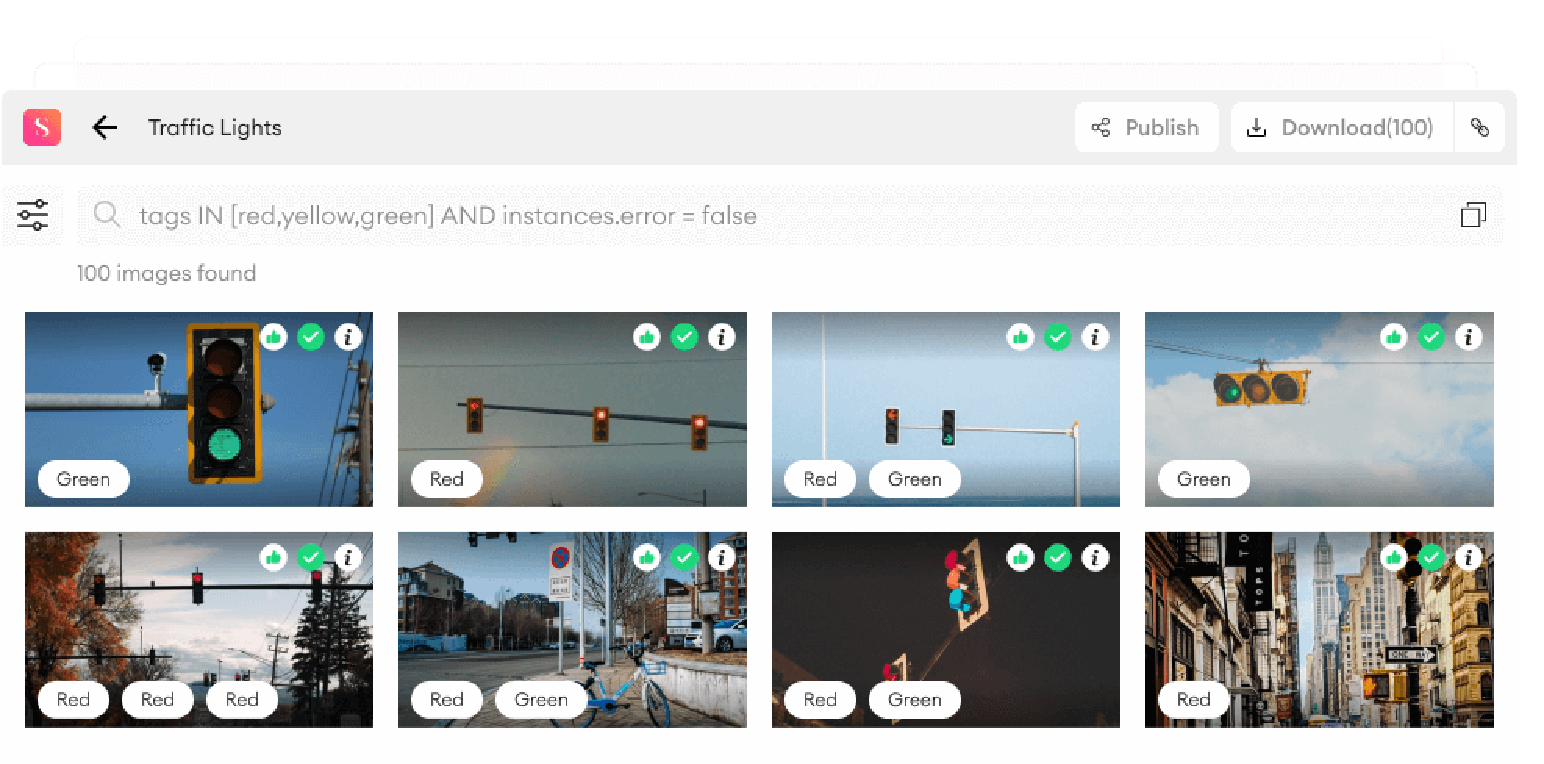
\includegraphics[width=1\textwidth]{figures/superannotate_interface.pdf}
    \caption{Relevance assessment of the concept "Traffic Lights" using SuperAnnotate's interface}
    \label{fig:superannotate_interface}
\end{figure}


% \section{The Bigger Picture}
% Exploring the background of the project through a review of the history and past accomplishments within the field is essential to establish its relevance and reason for existing. Looking at current solutions to the problem and their contrasting approaches provides valuable insight into which direction we take our project. Nevertheless, it is equally important to envisage the potential applications of our project beyond its primary focus of automated videography. For this reason, we look into recent research that aims to reduce relevance assessment efforts by employing query-specific variable depth pooling (CITE).


\section{Summary}
Exploring the background of the project through a review of the history and past accomplishments within the field is essential to establish its relevance and reason for existing. Looking at current solutions to the problem and their contrasting approaches provide valuable insights into the direction we should take our project. This is made explicit by our explorative dissection of the previous system as we propose potential solutions for its limitations. The advent of OpenAI's CLIP and Whisper \citep{whisper} models allow for a unique approach to the videography pipeline that could expand its current capabilities.

Regarding the annotation interfaces, both applications we reviewed share an intuitive interface design including clear checkmarks to indicate images tagged as relevant by the user. Nonetheless, even with the vast feature set that these systems offer, it still requires a lot of manual effort to complete the presented task in this project. To exemplify, the assessor must first listen and transcribe an audio source and subsequently input and annotate every segment within the transcript one by one. We believe our solution could streamline this procedure by automating the transcription process and making it easier to view and assess different audio segments within the interface itself.


%==================================================================================================
\chapter{Analysis/Requirements}
\label{chap:requirements}
This chapter serves to break down the high-level aims of the project in order to produce a list of functional and non-functional requirements, ordered by priority. This will directly determine the design and implementation of the project.

\section{Requirement Elicitation}
In order to elicit the list of requirements, a number of user scenarios are created. These are imagined scenarios of users that would directly benefit from such an application. This type of requirements gathering, most commonly used in agile software development projects, places the focus on the end-user, rather than the developer. Therefore, this prioritises the features that an end-user requires to fulfill their goals rather than designing the development process around what is easy to implement. Another benefit of this method is that it mitigates the risk of potential flaws at a very early stage. It is much easier to accommodate any flaws before any design or implementation is undertaken rather than finding them out during the evaluation stages with real users. 
% It gets progressively more difficult to change the existing design the further we are down the development process.


\subsection{User Scenarios}
\subsubsection{User Scenario 1: Anna} is a young secondary school teacher who has started recording her classes in response to the recent shift in online learning. She regularly posts her recordings to an online platform supported by the school. However, she has had a few complaints from her students that her recordings are not engaging enough and that it is difficult to see what she writes on the board. Anna strives to provide the best for her students and wishes she could make her recordings more engaging by illustrating the concepts she talks about in her audio recordings. However, she does not know anything about video production and is worried about the time required to learn and edit videos daily. She wishes for a tool that automatically illustrates her audio recordings in a swift manner. The created video should include captions to make it as accessible as possible for her students.

\subsubsection{User Scenario 2: William} has recently built two new automated video generation tools that use differing reranking procedures to retrieve the top images from the text. He has performed some user studies, where he asked a number of users to watch and rate the videos generated by both systems on the same audio tracks. He used A/B testing in order to compare the performances of his two systems. However, the user studies resulted in very mixed results, with some users rating system $A$ highly while others rated system $B$ as better. Furthermore, upon closer inspection, he found that the user ratings varied wildly depending on the audio tracks present in the videos. This was problematic since the user studies took over 2 hours to complete and William is unwilling to conduct another when it is unclear if the results would even improve with new participants. William wished that he could objectively evaluate his systems against a fixed test collection of ground-truths. He would be able to use this to obtain quantitative metrics for each system, giving a clear answer to which reranking procedure performs better.

\subsubsection{User Scenario 3: Lucy} is a software developer who is part of a small team building a new videography tool. Her manager has given her the tedious task of assessing the relevance of images for a predetermined set of audio from videos sourced from YouTube. This process requires manually annotating images that are the most fitting for the textual content existing within the audio. This is a very lengthy process since she must listen to the audio track multiple times in order to accurately transcribe the textual content. Following this, she must manually record the locations of the annotated images in a spreadsheet. Her manager has also assigned a colleague to double-check each annotation made. She wishes for a tool that automatically transcribes the audio and provides an easy-to-use interface to annotate relevant images. She requires that this ground-truth could be downloaded in a readable format for presenting to her manager. Additionally, it would be helpful to be able to edit the annotations after the fact, so that her colleague can fix any incorrectly judged images.


\subsection{User Stories}
\begin{itemize}
    \item \emph{As a user} of the application, \emph{I want to} upload audio files, \emph{so that} I can generate a video for it.
    \item \emph{As a user} of the application, \emph{I want to} specify YouTube video URLs, \emph{so that} its extracted audio can be used as the source.
    \item \emph{As a user} of the application, \emph{I want to} build and export a test collections for audio sources, \emph{so that} I can use them to evaluate my system.
    \item \emph{As an user} of the application, \emph{I want to} edit previously made annotations, \emph{so that} I can fix any mistakes made.
    \item \emph{As a user} of the application, \emph{I want} to view the full audio transcription, \emph{so that} I can annotate specific parts of the audio.
    \item \emph{As a user} of the application, \emph{I want to} view and download the generated video, \emph{so that} I can share it and upload it to any platform.
\end{itemize}


\section{Requirements}
In order to formalise and prioritise the main requirements identified, the MoSCoW method \citep{clegg1994moscow} was chosen. While it would be desirable to develop every feature that could help achieve the project's goal, the project's limitations make it impractical. Therefore, it is crucial to assess each feature's importance by evaluating how much it would contribute to achieving the intended goal. Each feature will fall into one of four categories:

\begin{itemize}
    \item \textbf{Must Have:} These are essential features that must be implemented to fulfill the project's aim.
    \item \textbf{Should Have:} These features are highly desirable, but missing them will not directly lead to a project failure.
    \item \textbf{Could Have:} These are features that are beneficial but are viewed as extra perks.
    \item \textbf{Won't Have:} These features are not worth pursuing.
\end{itemize}

The list is divided into two sections: Functional Requirements, which describe interactive features, and Non-Functional Requirements, which describe program properties that users cannot interact with. Requirements marked by an \textbf{*} were added at later stages in the project development as new feature ideas emerged.

\subsection{Functional Requirements}
\begin{enumerate}
    \item \label{req:1} \textbf{Must Have:} The ability to upload an audio file as an input audio source.
    \item \label{req:2} \textbf{Must Have:} The ability to specify a YouTube video URL as an audio source.
    \item \label{req:3} \textbf{Must Have:} The ability to view the full audio transcription.
    \item \label{req:4} \textbf{Must Have:} The ability to generate an illustrated video for any audio source.
    \item \label{req:5} \textbf{Must Have:} The ability to view the top-$k$ retrieved images for a given audio chunk.
    \item \label{req:6} \textbf{Must Have:} The ability to annotate the most-fitting images for a given audio chunk.
    \item \label{req:7} \textbf{Must Have:} The ability to view the text present in a given audio chunk.
    \item \label{req:8} \textbf{Must Have:} The ability to view the constructed ground-truth data.
    \item \label{req:9} \textbf{Must Have:} The ability to download the constructed ground-truth data in a portable, human-readable format.
    \item \label{req:10} \textbf{Should Have:} The ability to view previously processed audio sources, generated videos, and constructed ground-truth.
    \item \label{req:11} \textbf{Should Have:} The ability to edit previously made ground-truths.
    \item \label{req:12} \textbf{Should Have:} The ability to upload audio sources of any language.
    \item \label{req:13} \textbf{Could Have:} The ability to load ground-truths for editing.
    \item \label{req:14} \textbf{Could Have:} The ability to reconfigure the static image collection.
    \item \label{req:15} \textbf{*Could Have:} The ability to view the percentage complete for ground-truth construction of processed audio sources.
    \item \label{req:16} \textbf{*Could Have:} The ability to save or skip chunks with repeating textual content when ground-truth constructing.
    \item \label{req:17} \textbf{*Could Have:} The ability to view the timestamp information of audio chunks.
\end{enumerate}

\subsection{Non-Functional Requirements}
\begin{enumerate}[resume]
    \item \label{req:18} \textbf{Must Have:} The system using a static collection of images for repeatably consistent ground-truth construction.
    \item \label{req:19} \textbf{Should Have:} The application being accessible from any Operating System platform.
    \item \label{req:20} \textbf{Should Have:} The application having a presentable user interface that is easy for any user to understand and learn quickly.
    \item \label{req:21} \textbf{Should Have:} The application with appropriate error handling.
    \item \label{req:22} \textbf{Should Have:} The application being fast and responsive.
    \item \label{req:23} \textbf{Should Have:} The system being able to recognise music tracks to automatically retrieve the artist name and song title.
    \item \label{req:24} \textbf{Should Have:} The application being able to transcribe any audio source providing phrase-level timestamps.
    \item \label{req:25} \textbf{Should Have:} The system retrieving more relevant images by leveraging semantics of natural language as well as visual features.
    \item \label{req:26} \textbf{Should Have:} The videos being generated in a more reasonable amount of time than the prior system.
    \item \label{req:27} \textbf{Should Have:} The generated video having a higher resolution than the prior system.
    \item \label{req:28} \textbf{Should Have:} The application displaying progress bars for long loading times.
    \item \label{req:29} \textbf{Could Have:} The application being designed with extensibility in mind so that the image collection can be reconfigured.
    \item \label{req:30} \textbf{Could Have:} The videos including text as well as images.
    \item \label{req:31} \textbf{Could Have:} The application visually differentiating between previously processed audio sources.
    \item \label{req:32} \textbf{Could Have:} The system performing tempo or beat analysis to appropriately time image changes.
\end{enumerate}


\section{Summary}
This chapter presented a detailed outline of the essential features for the project's development. The approach involved crafting user scenarios and stories to gain insight into potential user needs, thereby deriving a MoSCoW prioritised list of requirements. This process provides greater clarity for the ensuing stage of the project - Design.

% What is the problem that you want to solve, and how did you arrive at it?
% \section{Guidance}
% Make it clear how you derived the constrained form of your problem via a clear and logical process. 

% The analysis chapter explains the process by which you arrive at a concrete design. In software 
% engineering projects, this will include a statement of the requirement capture process and the
% derived requirements.

% In research projects, it will involve developing a design drawing on
% the work established in the background, and stating how the space of possible projects was
% sensibly narrowed down to what you have done.

%==================================================================================================
\chapter{Design}
This chapter serves to provide the initial design choices including a high-level view of the system workflow and the wireframes of the intended user interface. All decisions will be explained with a general aim to optimise the user experience and fulfill the identified system requirements. Next, a deeper look into the design choices of the internal workings of components. This allows our system to be implemented in any language while maintaining clean and agile software design principles. 

\section{High-Level Plan of System}
In order to start planning out the workflow of our system, it is necessary to simplify and abstract the key components that make up the backbone of the system. Our system is comprised of two sub-systems, an automatic videography tool, and a ground-truth annotation tool. However, both sub-systems use the same underlying pipeline. The simplified workflow diagram displayed as Figure \ref{fig:simplified_workflow} shows the basic, black-boxed components that make up our pipeline: a \textbf{transcription extractor}, a \textbf{video generator}, and an \textbf{annotation interface}.

The user inputs an audio source which is processed to extract a synced transcription of the audio content. Next, the user has the option to either choose to generate a video or start constructing the ground-truth for it. Each option produces an output that the user can subsequently view and export. In line with the requirements, these outputs are saved to the database for future editing.

\begin{figure}[h]
    \centering
    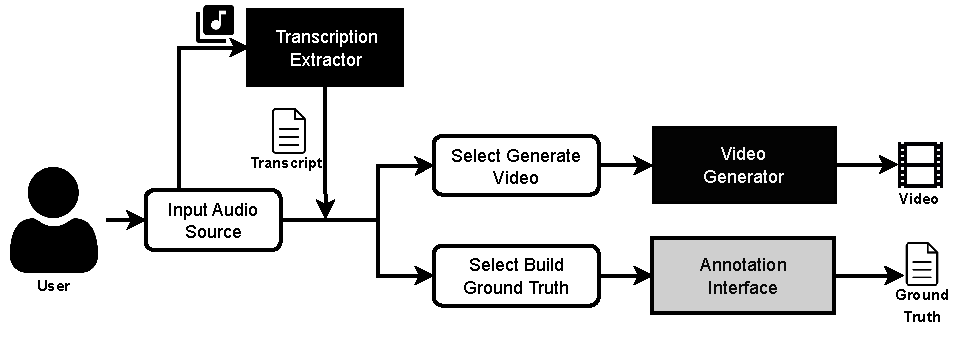
\includegraphics[width=1\textwidth]{figures/simplified_architecture.pdf}
    \caption{Simplified workflow diagram showing the basic high-level design of the system}
    \label{fig:simplified_workflow}
\end{figure}

\subsection{Transcription Extractor}
Firstly, the user inputs an audio source. As stated in the requirements, this can either be in the form of a YouTube video URL or a direct upload of an audio file. This input is passed along to the Transcription Extractor. This component produces a transcription of the audio with phrase-level timing information. It is vital that this transcription is synced accurately with the audio since this information will be used to place relevant images during video compilation.

There are a number of ways to retrieve the synced transcription, firstly, we can leverage YouTube's captioning system if the user chooses to input a YouTube video URL. However, we cannot always rely on this since captions are not guaranteed to be present. Secondly, for music, it is possible to retrieve synced lyrics from open-source databases, which requires identifying the artist name and track title. In order to avoid the YouTube metadata problem from the previous thesis (\ref{par:metadata_problem}) and allow this to function for uploaded audio files, we must process the audio to recognise and retrieve the track information. Finally, we require a backup audio-to-text transcription tool for non-music audio sources or YouTube videos containing no captions. This workflow is depicted in Figure \ref{fig:transcription_extractor}.

\begin{figure}
    \centering
    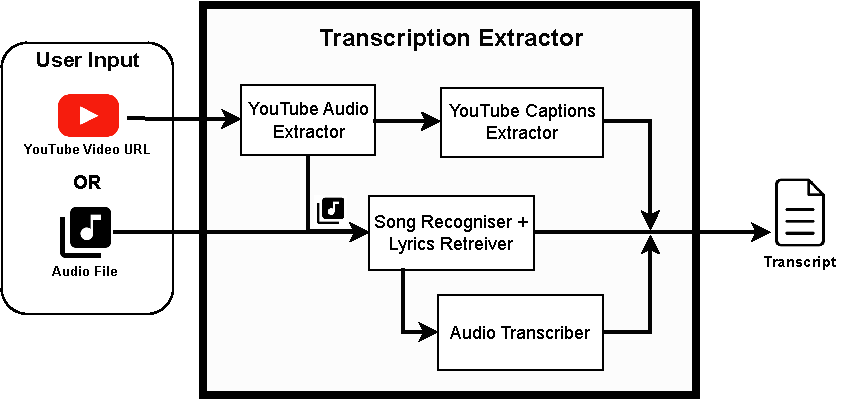
\includegraphics[width=0.8\textwidth]{figures/transcription_extractor.pdf}
    \caption{Internal view of the Transcription Extractor component}
    \label{fig:transcription_extractor}
\end{figure}

\subsection{Video Generator}
This component should activate when the user chooses to generate a video. It takes in the audio and the synced transcription which is divided into phrase-level chunks. Next, the videography tool should retrieve the top-$1$ relevant image for each chunk and sequence them into a video according to the timestamp information present. The audio should then be added to the rendered video which will subsequently be outputted for the user to view and export. Since, it is common for some phrases to be repeated, especially in music, we may want to retrieve different images for each repeated phrase. Our main goal is to produce a video that is engaging to the user. In these cases, we can simply retrieve the next relevant image in our collection.

\subsection{Annotation Interface}
The annotation interface consists of a system workflow of its own since the user will be actively interacting with the interface in order to incrementally construct the ground-truth for the audio. Figure \ref{fig:annotation_interface} presents the workflow that an annotator would follow.

\begin{figure}[h]
    \centering
    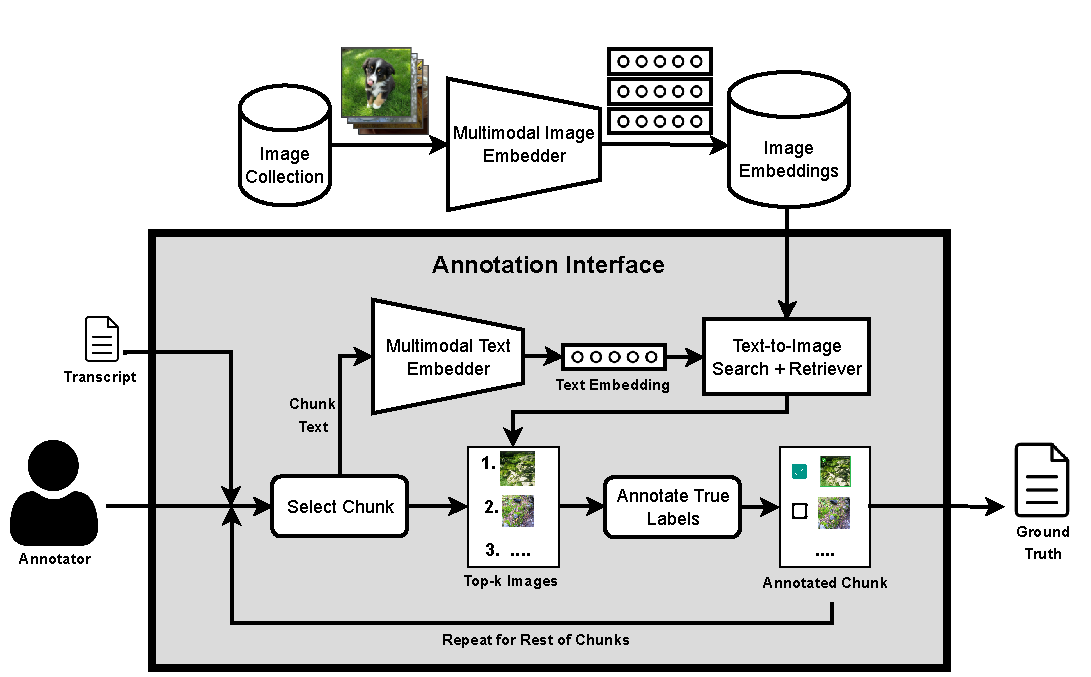
\includegraphics[width=0.95\textwidth]{figures/annotation_interface.pdf}
    \caption{Internal view of the Annotation Interface architecture}
    \label{fig:annotation_interface}
\end{figure}

Since one of our requirements specifies a static image collection (Requirement \textbf{\#\ref{req:18}}), this gives the benefit of being able to pre-process the entire collection since we know that the images are not going to change. Additionally, as we want to include the semantics of text and images, we must embed all the images into a multimodal space into which text can also be embedded into.

Firstly, the annotator would select an audio chunk to assess. This freedom to choose which part of the audio to annotate is essential in order to facilitate the requirement of editing annotations (\textbf{\#\ref{req:11}}). However, it can be assumed that the annotator will construct the ground-truth in the order of the audio. Once a chunk is selected, the top-$k$ images are retrieved and shown to the assessor by embedding the chunk text and performing a search in the multimodal vector space. The annotator is then expected to identify and label the images that they judge as the most fitting to the chunk text. This procedure will be repeated for every chunk of the audio until a completed ground-truth set is constructed. This is subsequently outputted to the annotator in an accessible format.


\section{User Interface Design}
The user interface (UI) is a critical part of our application due to its importance within our task specification. Hence, ensuring our design was intuitive even for untrained users, to enable the freedom to crowdsource proved to be a challenge. Competing in the field with major annotation platforms only mounted more incentive to design an interface that is unique yet familiar. Furthermore, it was important to ensure pages within the UI remained uncluttered. For this reason, before any development commenced, we started prototyping interface designs using \cite{figma}.

\subsection{Home Page}
The simplified workflow outlined in Figure \ref{fig:simplified_workflow} is used as the basis to form the various pages within the application. Firstly, we require a page for the user to enter the audio source to initiate the process. Hence, this 'Home' page requires a way for the user to upload an audio file from their local machine (\textbf{\#\ref{req:1}}), as well as a text field to take in a YouTube video URL (\textbf{\#\ref{req:2}}). Appropriate validation is necessary to handle erroneous inputs such as incompatible file formats or URLs not from the YouTube domain. More importantly, these errors should be clearly displayed to the user so that they can respond accordingly. An initial design of the Home page can be seen in Figure \ref{fig:home_page}. 

In addition to taking inputs from the user, we also include a navigation bar with intended links to an 'About' page and a 'Collections' page. Since we want our application to be open to anyone wanting to generate videos or develop ground-truths, we believe an About page is necessary to provide information about the interface and how to use it. The idea of a Collections page was spawned to satisfy the potential to save processed audio sources and generated videos (\textbf{\#\ref{req:10}}). Furthermore, since these links are required to be easily accessible, we include this navigation bar on subsequent pages.

\begin{figure}
    \centering
    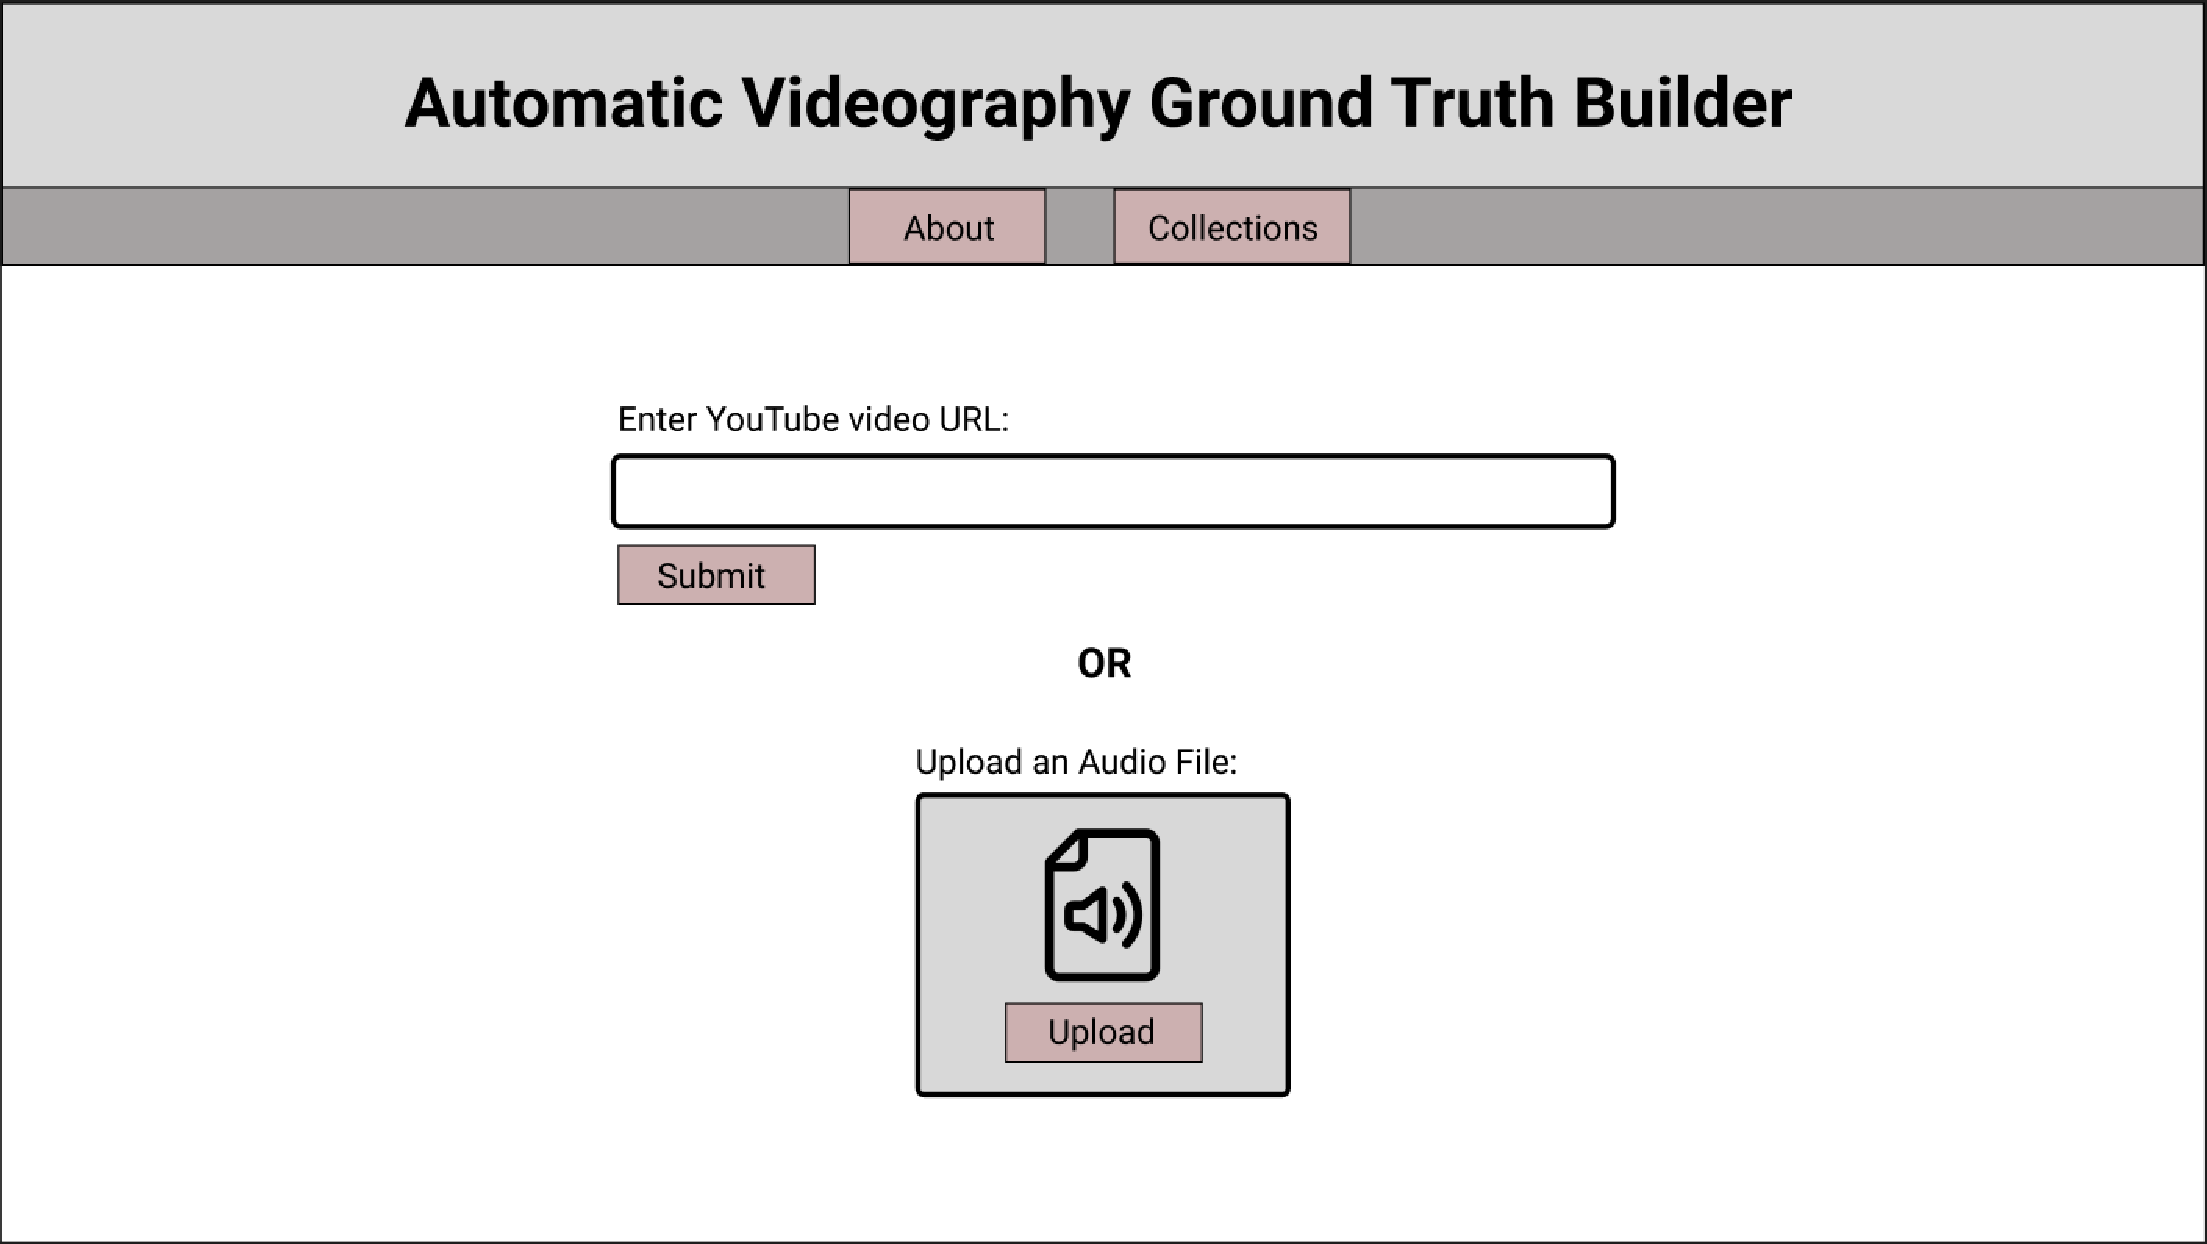
\includegraphics[width=0.95\textwidth]{figures/home_page.pdf}
    \caption{An initial prototype for the Home page, illustrating how the user can input an audio source.}
    \label{fig:home_page}
\end{figure}

\subsection{Audio Page}
Once the audio source is submitted, the Transcription Extracter component should produce a full transcription of the audio. This should lead to the next page displaying the results of the audio processing with the two different options of where to proceed next. More specifically, the user can choose to generate the video with the 'Generate Video' button, or start constructing a ground-truth with the 'Build Ground Truth' button. The full transcription should also be shown to fulfill requirement \textbf{\#\ref{req:3}}. 

Aside from this, to save the audio processing result in a database, it must be uniquely identifiable. This led to the idea of associating the audio source with a Title and an optional Author. In the case where the audio is sourced from a file uploaded by the user, the title can simply be the filename. Whenever the audio is extracted from a non-music YouTube video, the title and author can be taken from the YouTube metadata. Finally, for music tracks, the title and author fields can be filled with the recognised track information such as the song title and artist name respectively. Our design, shown in Figure \ref{fig:audio_page}, also includes an associated image since we believe this could be visually appealing and satisfy the requirement to be able to differentiate collected audio sources (\textbf{\#\ref{req:31}}). This could simply be the video thumbnail for YouTube sources, while for music tracks, the image field can be satisfied by their corresponding cover art. 

\begin{figure}
    \centering
    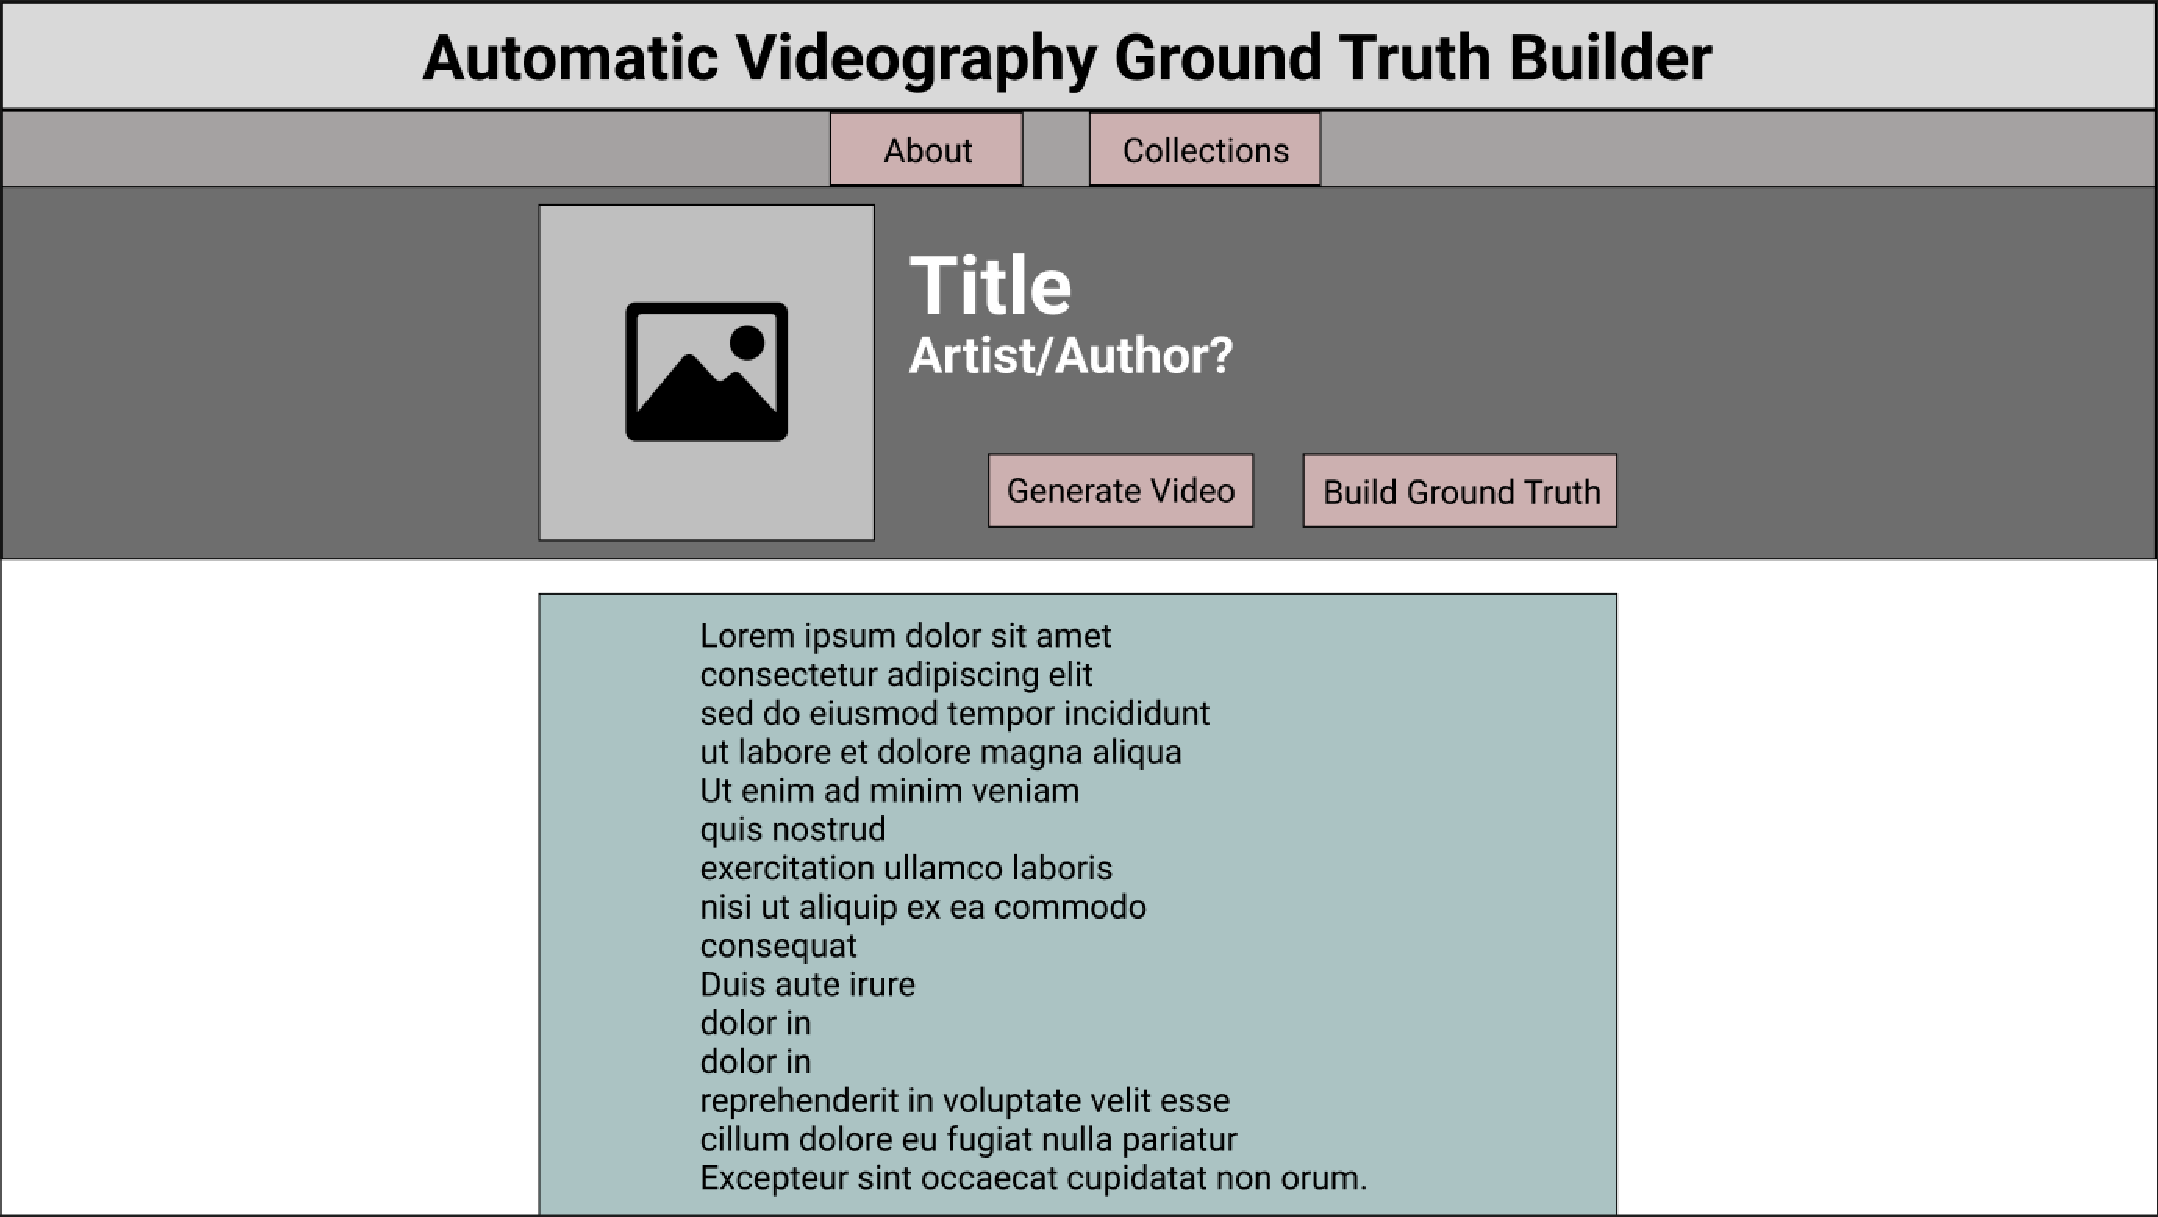
\includegraphics[width=0.95\textwidth]{figures/audio_page.pdf}
    \caption{An initial prototype for the Audio page showing the resulting transcript after processing the audio.}
    \label{fig:audio_page}
\end{figure}

\subsection{Video Page}
The Video page is rendered when the user clicks on the 'Generate Video' button from the Audio page. This page provides an embedded video so that the user could view the video on the interface itself instead of forcing them to download it to view it. This page will be minimalistic in design, as illustrated in Figure \ref{fig:video_page}, and the 'Author - Title' divider will be utilised as the link back to the Audio result page. Once the video is generated, this will be saved in the backend for easy access. Prior to the rendering of this page, we intend to provide a descriptive loading screen since it is expected that the video compilation will take several minutes as made evident by the previous system. This intermediate loading page adheres to our listed requirements (\textbf{\#\ref{req:28}}) giving an estimated time of completion while simultaneously preventing the user from interacting with other parts of the interface during video generation.

\begin{figure}
    \centering
    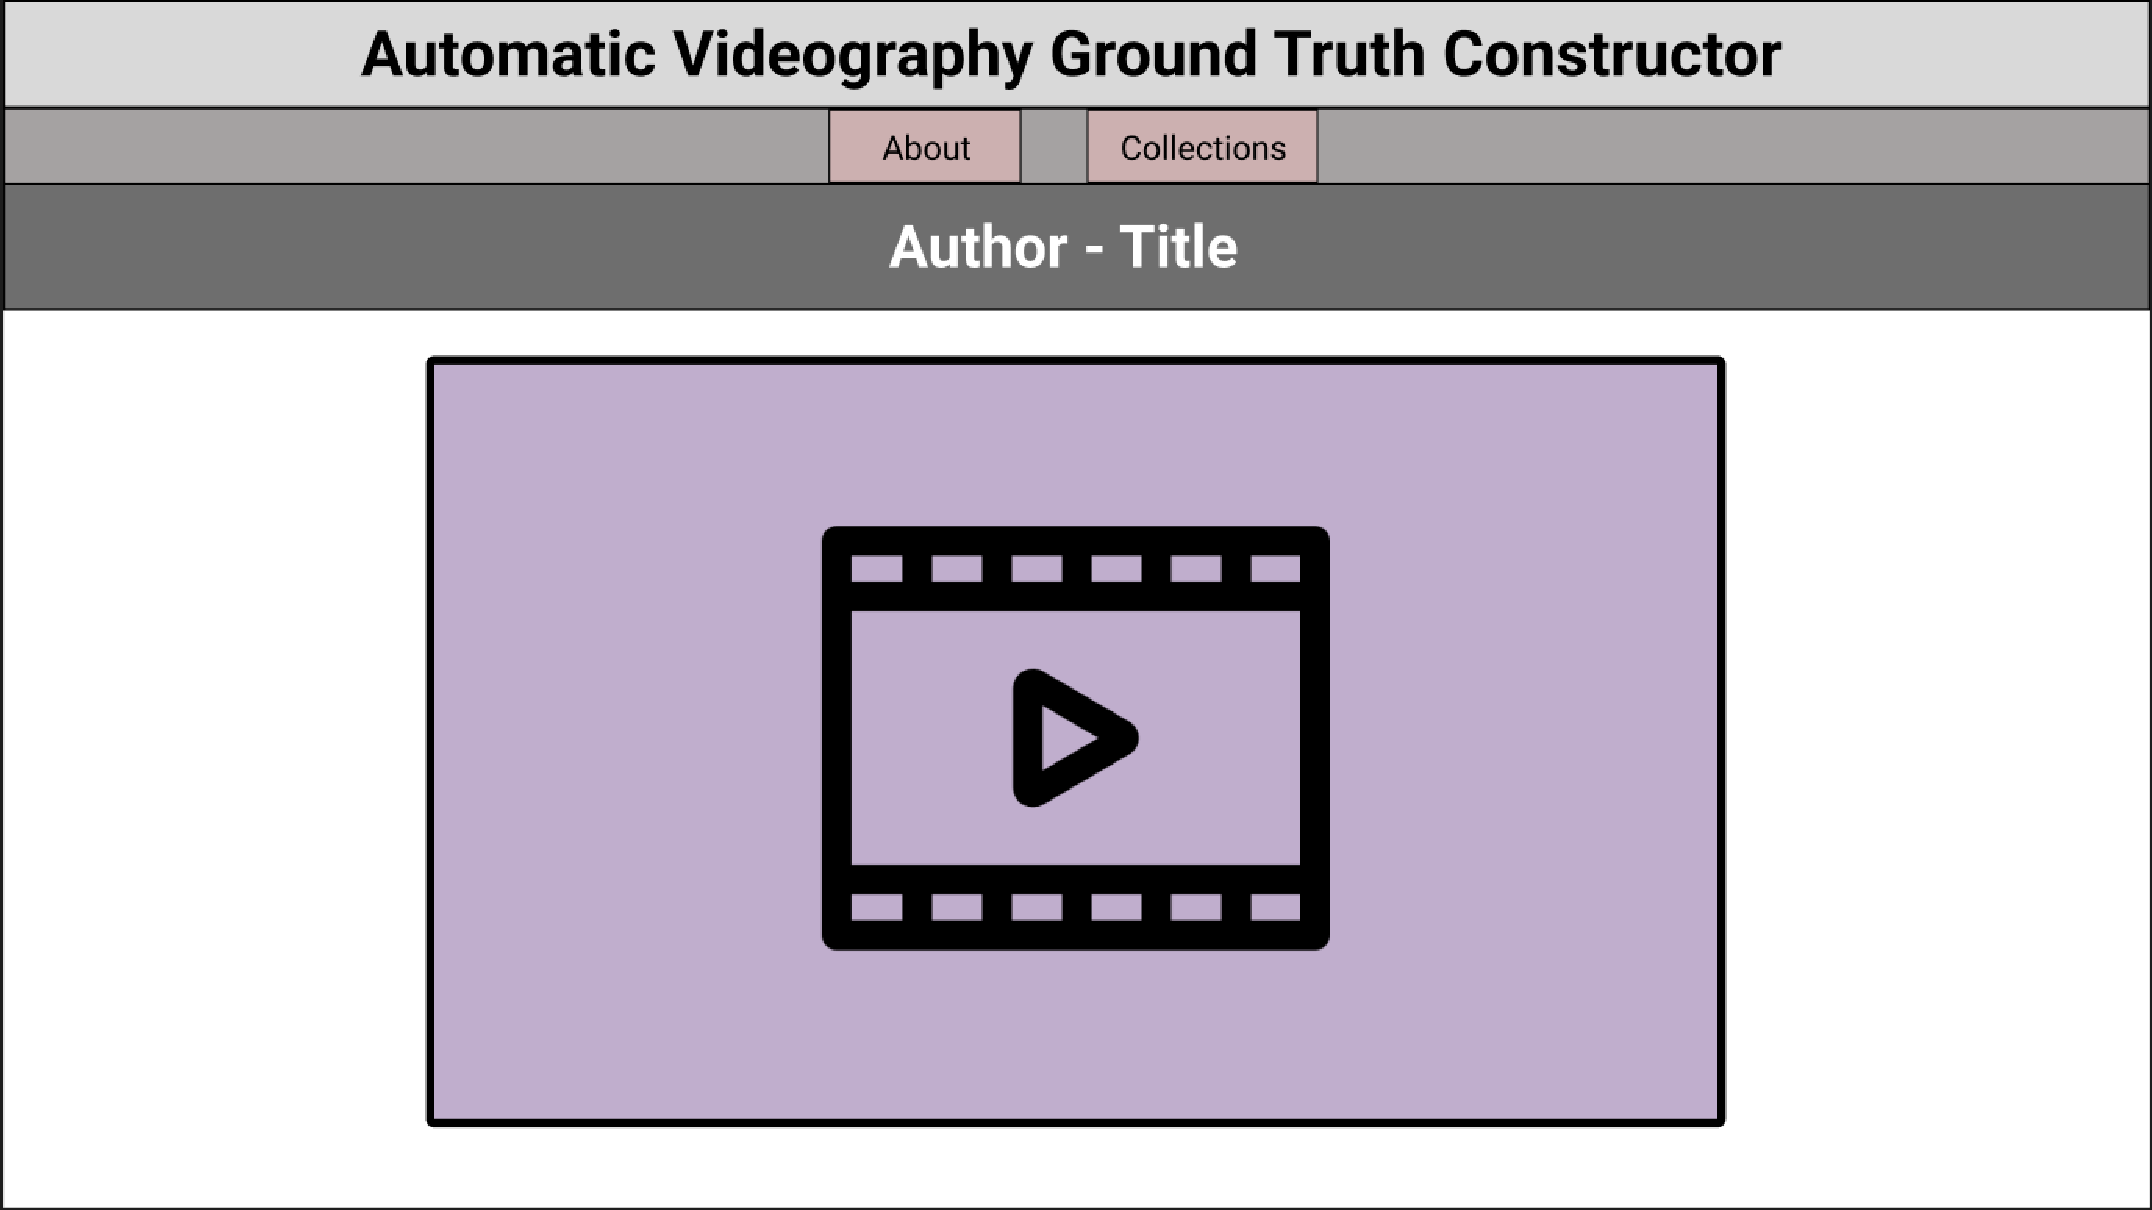
\includegraphics[width=0.95\textwidth]{figures/video_page.pdf}
    \caption{An initial prototype for the Video page providing the generated video.}
    \label{fig:video_page}
\end{figure}

\subsection{Chunk Page}
Alternatively, the user can choose to construct the ground-truth for the audio source by clicking on the 'Build Ground Truth' button on the resulting Audio page. This should subsequently navigate the user to the first audio chunk page. This should show the text present within that chunk and the retrieved top-$k$ images using the system (\textbf{\#\ref{req:5}}, \textbf{\#\ref{req:7}}). As seen in Figure \ref{fig:chunk_page}, we picked a depth $k=10$ since it is small enough for the assessor to efficiently comb through for the most relevant images. This is especially true when this task must be repeated for every chunk in the audio source. We want to avoid a burdensome experience that could affect the quality of relevance assessments. However, we found that this cut-off point is highly dependent on the effectiveness of the retrieval system as well as the textual query, further discussed in \ref{sec:determining_pool_depth}.

\begin{figure}
    \centering
    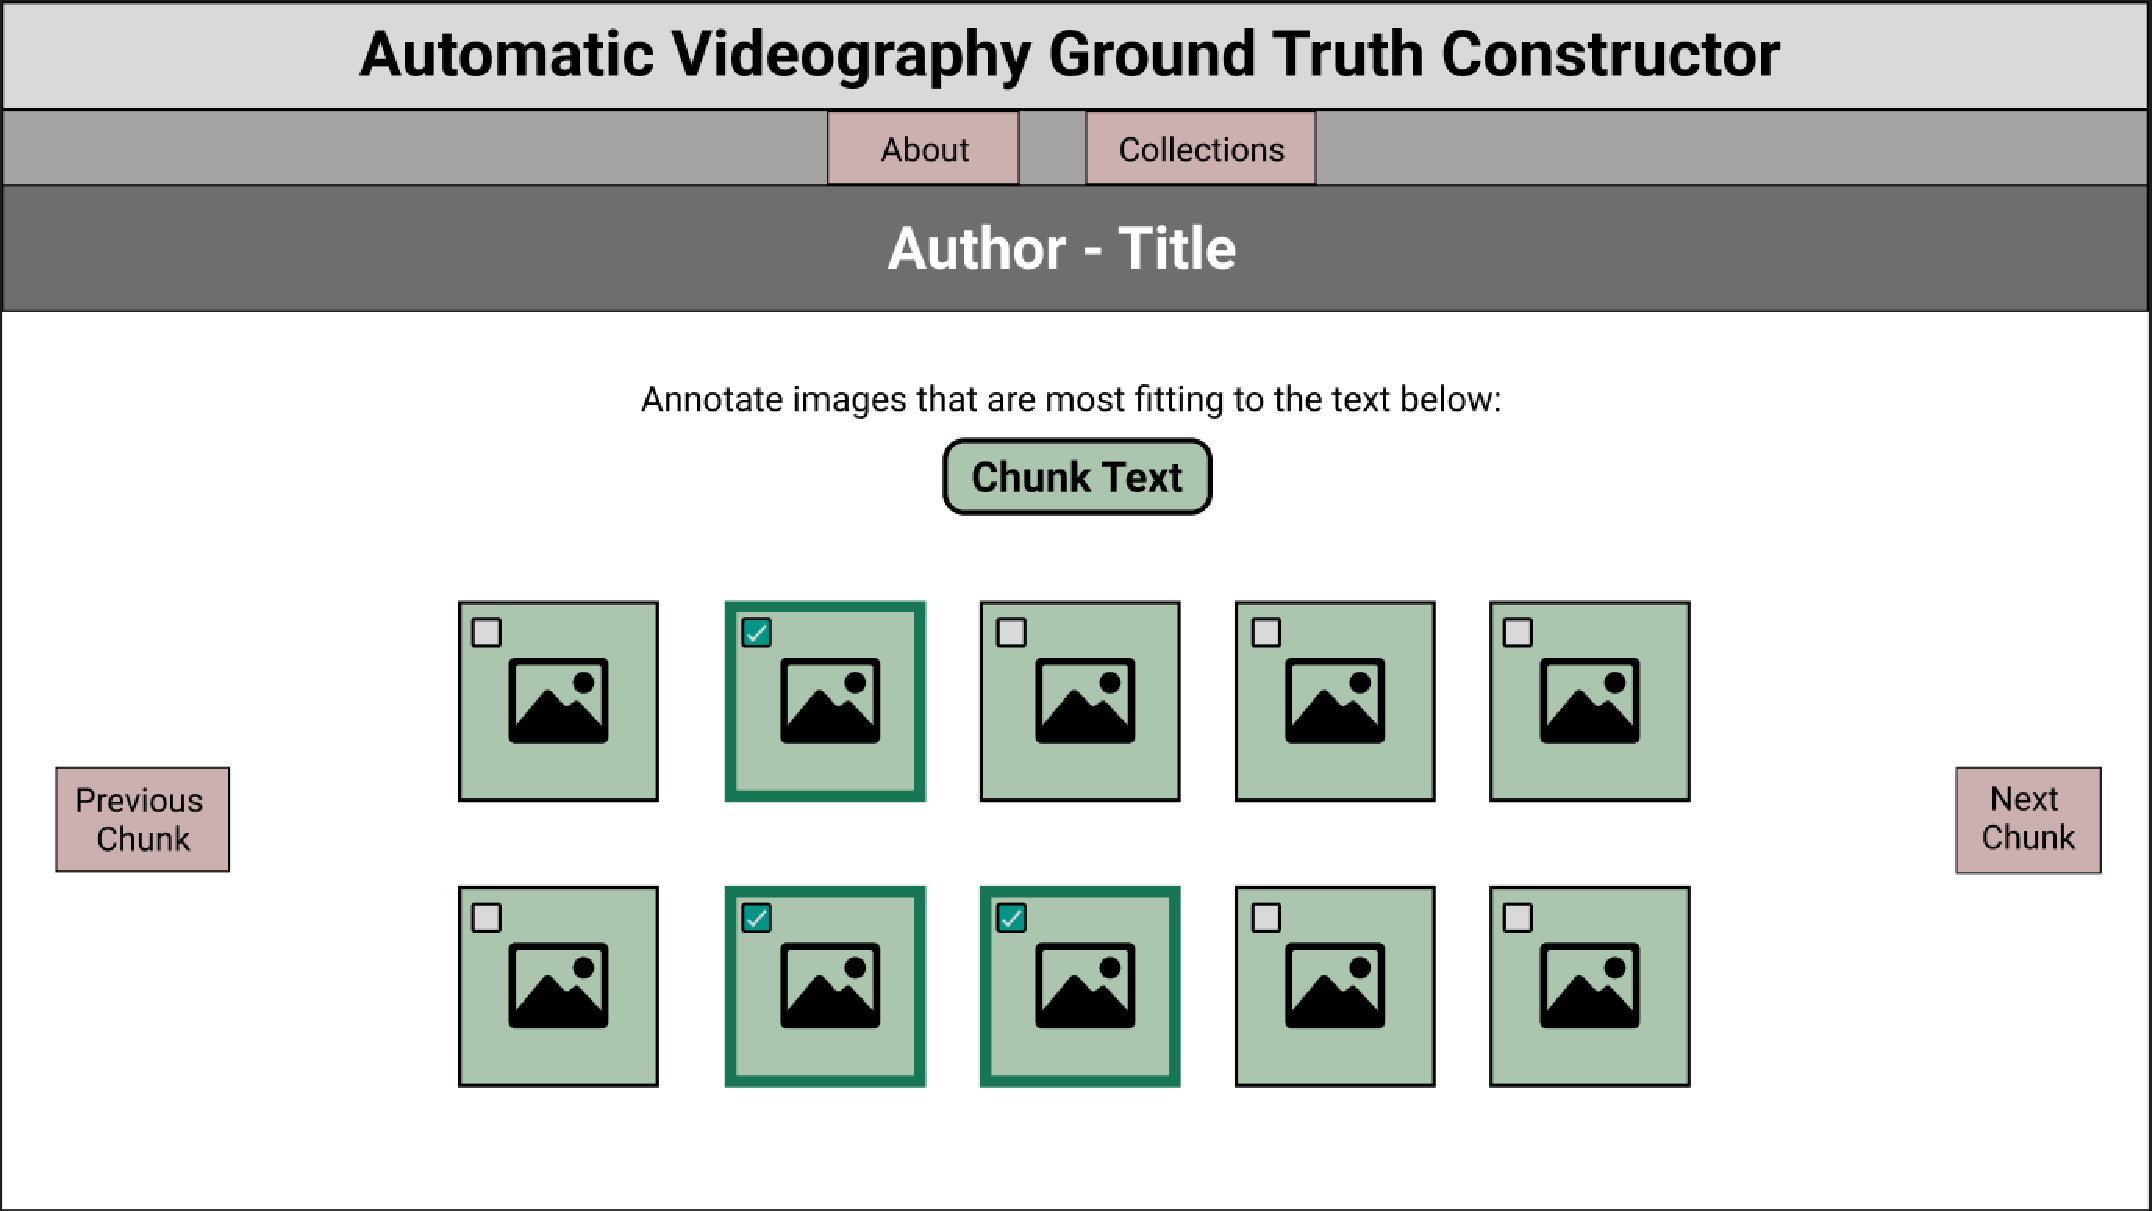
\includegraphics[width=0.95\textwidth]{figures/chunk_page.pdf}
    \caption{An initial prototype for the Chunk pages that provide the ability to assess the relevance of retrieved images for specific audio chunks.}
    \label{fig:chunk_page}
\end{figure}

We chose to use a binary relevance assessment strategy where the assessor must only mark relevant images meaning unmarked images are considered irrelevant (\textbf{\#\ref{req:6}}). This is faster than a graded relevance system which requires significant thought and may discourage accurate assessments. This is also backed by approaches employed by similar technologies (\ref{sec:labelbox} \& \ref{sec:superannotate}). In addition to these interactive images, the page includes 'Previous' and 'Next' buttons to easily navigate to bordering chunk pages. We also aspire to save the user's assessments when these buttons are pressed in order to reduce annotation effort and allow editing of previous chunks (\textbf{\#\ref{req:11}}). Not to mention to allow the possibility of skipping chunks with repeating textual contents (\textbf{\#\ref{req:16}}).

\subsection{Ground-Truth Page}
Once all audio chunks have been annotated, the system should render a resulting Ground-Truth page similar to Figure \ref{fig:ground_truth_page}. This consists of a small preview of the ground-truth data and some functionality to download the constructed data (\textbf{\#\ref{req:8}}, \textbf{\#\ref{req:9}}). While the ground-truth data may be technical, we intend to deliver it in a human-readable format so that assessors can perform last-minute checks if required. The preview feature also enables retrieval system designers to peek at the format of the ground-truths to aid in the evaluation process.

\begin{figure}[H]
    \centering
    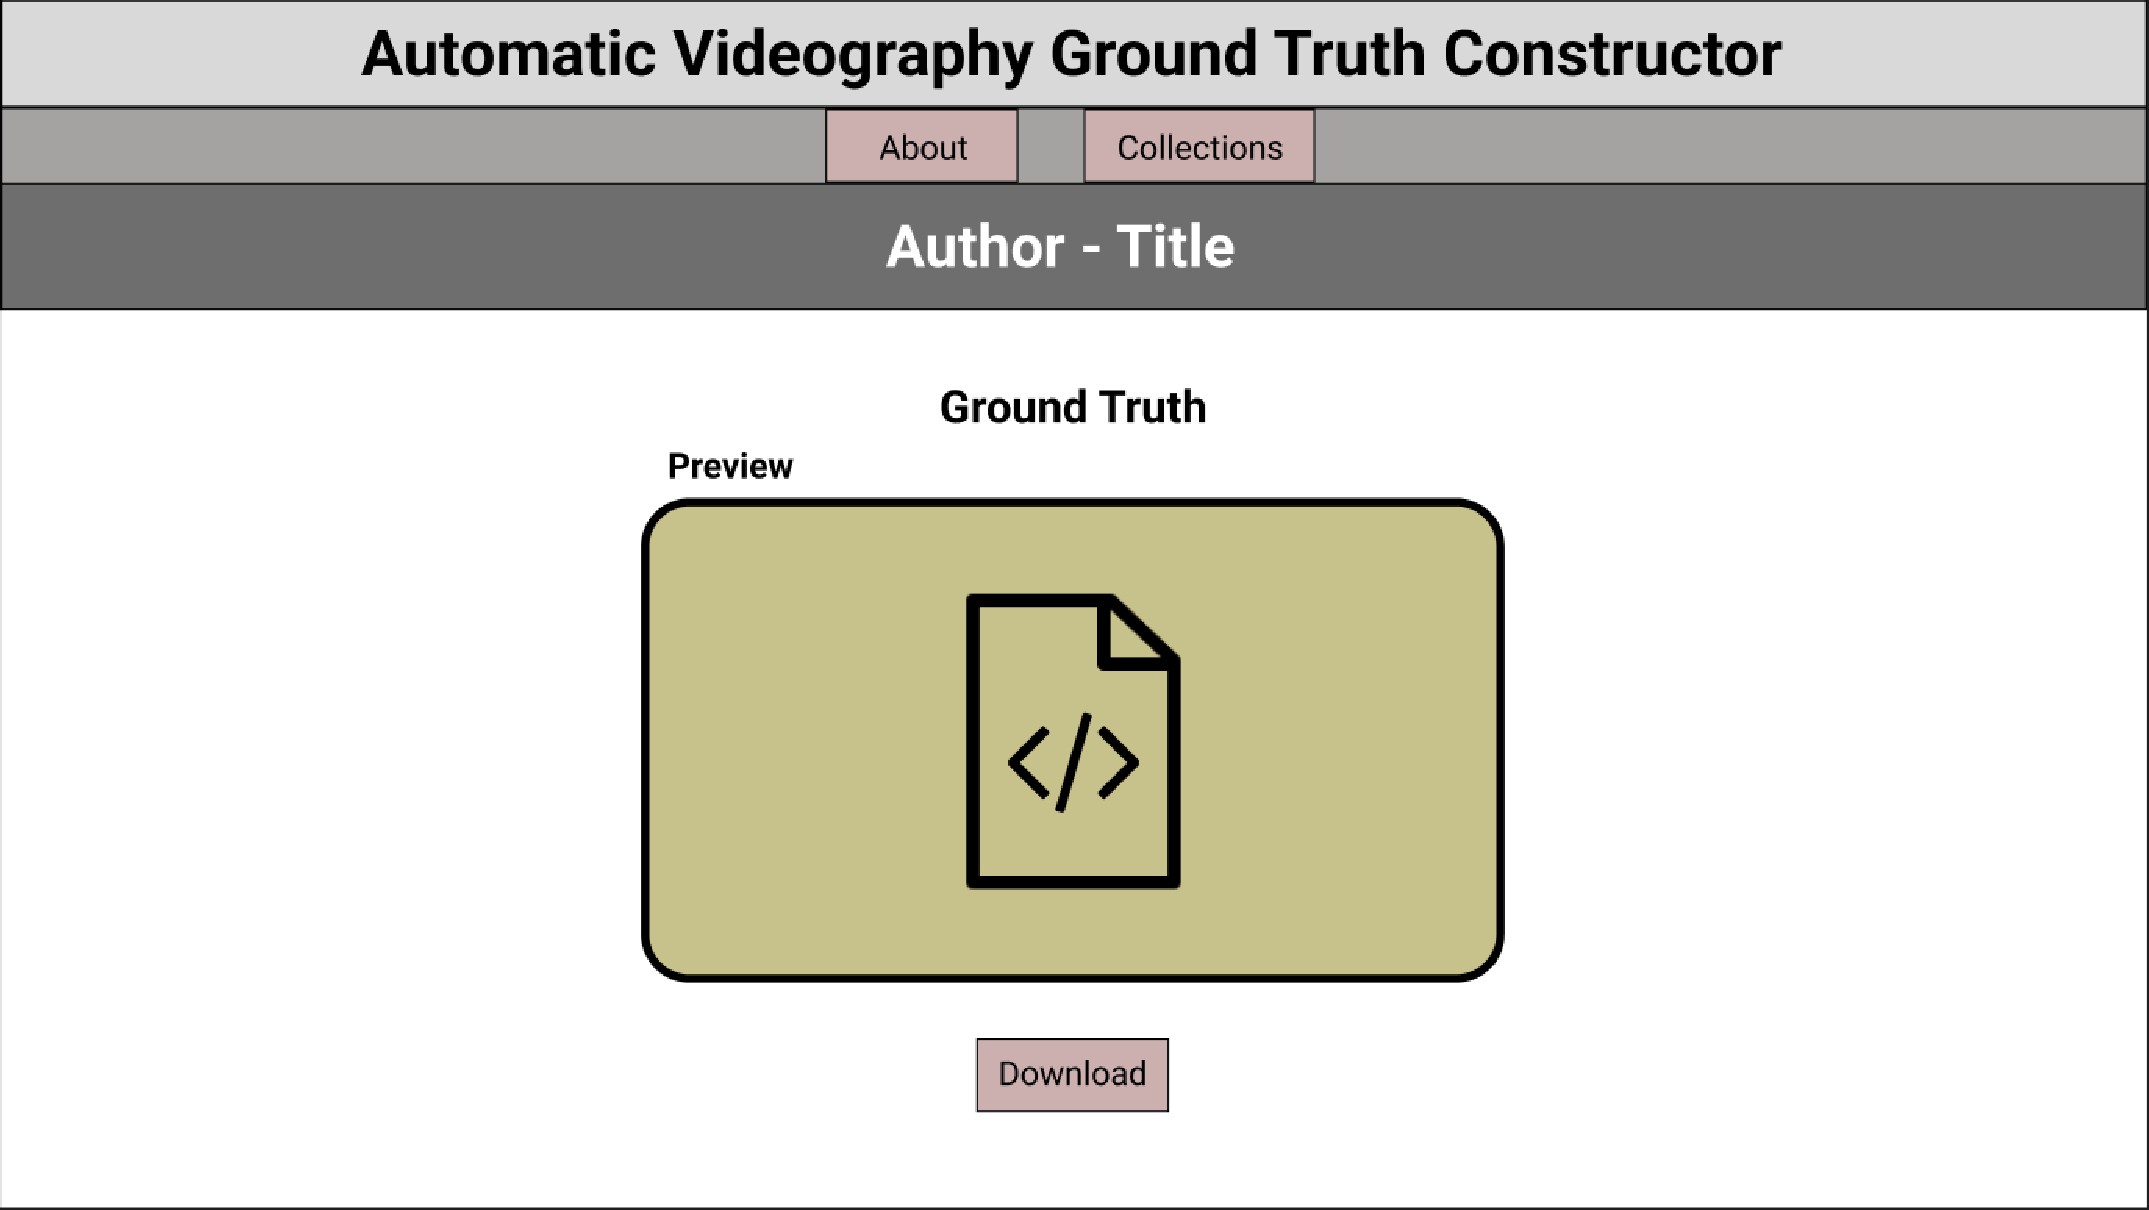
\includegraphics[width=0.95\textwidth]{figures/ground_truth_page.pdf}
    \caption{An initial prototype for the Ground-Truth Page providing a preview of the constructed ground-truth available for download.}
    \label{fig:ground_truth_page}
\end{figure}


\section{Summary}
This chapter provided a comprehensive overview of the design choices made across all areas within the project. From the system architecture to the high-level decisions of the user interface following best Human-Computer Interaction (HCI) design practices. Now that a detailed plan is in place, an intuitive entryway into actually implementing the project is uncovered, in a way that aligns with the requirements specification made in Chapter \ref{chap:requirements}. 

% How is this problem to be approached, without reference to specific implementation details? 
% \section{Guidance}
% Design should cover the abstract design in such a way that someone else might be able to do what you did, 
% but with a different language or library or tool. This might include overall system architecture diagrams,
% user interface designs (wireframes/personas/etc.), protocol specifications, algorithms, data set design choices,
% among others. Specific languages, technical choices, libraries and such like should not usually appear in the design. These are implementation details.


%==================================================================================================
\chapter{Implementation}
This chapter will provide a detailed look into the implementation of the project. The rationale behind all technology choices and their involvement to achieve our desired product will be explained here. 

\section{Software Development Process}
\subsection{Version Control}
\cite{github} was the chosen technology to host the remote copy of the repository and version control throughout the implementation. This ensured all code was regularly backed up, providing a layer of security against local data loss or corruption. In addition, it provided a detailed tracking of the project's development, allowing the freedom to go back to previous versions if necessary. Since this was an individual project every feature was developed sequentially making branching unnecessary due to the lack of potential merging conflicts. However, branching was utilised at the beginning of the project when it was unclear which direction the project should be taken. For instance, several options for the image collection were considered, most notably taking them from the \cite{wikimedia_commons} or \cite{imagenet}, each stored in separate branches.


\subsection{Application Framework and Language Choice}
It was decided the project should be developed as a web application due to the system requirement \textbf{\#\ref{req:19}}. A web application can be easily deployed to the internet making it accessible to everyone, irrespective of the device or operating system used. Additionally, it offers the advantage of eliminating the need to download and execute large files.

Python \citep{python} was the main programming language chosen due to its flexibility and a huge selection of libraries allowing rapid development in such a time-constrained project. Popular libraries such as NumPy \citep{harris2020numpy} offer a wide range of optimised functions for data processing and manipulation. Furthermore, this decision led to the idea of developing the web application using \cite{django}, a popular Python web framework.

Django follows a Model-View-Template (MVT) design architecture illustrated in Figure \ref{fig:django_architecture}. It consists of three fundamental components:
\begin{itemize}
    \item The \textbf{Model} manages the data stored in a relational database.
    \item The \textbf{View} communicates with both the model and template in order to complete and send back an HTTP\footnote{HTTP: Hyper-Text Transfer Protocol} response to the client, corresponding to their HTTP request.
    \item The \textbf{Template} acts as the frontend of the application providing dynamic HTML webpages to the client.
\end{itemize}

\begin{figure}
    \centering
    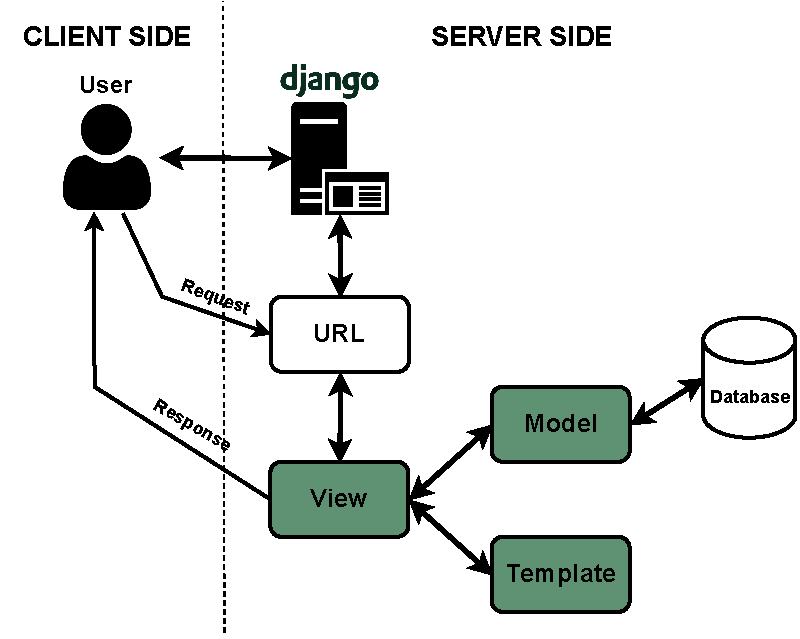
\includegraphics[width=0.7\textwidth]{figures/django_architecture.pdf}
    \caption{An architecture diagram showing the MVT design pattern of Django web applications.}
    \label{fig:django_architecture}
\end{figure}

Django has an intermediary component that catches the client's HTTP requests to pattern-match requested URLs to the correct view. The view then fetches data from the models stored in the backend, and renders a template back to the client.


\section{Backend Structure}
\subsection{Static Image Collection}
In line with requirement \textbf{\#\ref{req:18}}, several sources for image collections were considered. Out of those, there were two notable sources: the Wikimedia Commons and ImageNet. Wikimedia Commons hosts a range of images that are, more importantly, captioned with accurate textual descriptions. In addition to the latest multimodal, multilingual image-text dataset released by \cite{srinivasan2021wit}, a research group within Google. It appeared to be an appealing option as it allowed the flexibility to train our own image-text model using the provided textual descriptions. However, complications arose in downloading the dataset. We found that in order to save space, the dataset only included image URLs meaning that the images must be programmatically downloaded one by one. After weeks of testing, even going as far as parallelising the download process, we deemed this effort infeasible due to its slow pace. 

We ultimately decided on procuring the collection from ImageNet, an open-source image database containing over 14 million images, available in zipped formats. Moreover, it provided many smaller subsets of the dataset that allowed the chance to familiarise ourselves with CLIP's pre-trained model architecture. The ImageNet-1k subset was the chosen collection for our project which spanned over 1.1 million images allowing reasonable pre-processing times while also being large enough for satisfactory image retrieval results.


\subsection{Models}
Our application consists of only two models: Audio and Chunks. As depicted in the Entity Relation (ER) diagram in Figure \ref{fig:models_schema}, each Audio object consists of 0 or more Chunk objects. This was to accommodate purely instrumental audio tracks that would contain no spoken language. While this is not useful for our current application domain, we believed this feature could be expanded upon in future iterations where the audio content itself could be used in the image retrieval process using sentiment analysis.

\subsubsection{Audio}
The Audio model holds all information associated with inputted audio sources after processing is complete. This includes the artist/author's name, title, transcript, and the ground-truth data. A boolean flag for whether the audio is a music track or not is used to course the appropriate processing steps. The file name field is used to find corresponding files stored in the static directory, such as the audio, cover art image, and transcript files. 

\subsubsection{Chunk}
The Chunk model consists of specific information about the segment in the audio such as the text present, start and end times, as well as, the top-10 and annotated images. It also holds a foreign key that references the appropriate Audio object.

\begin{figure}
    \centering
    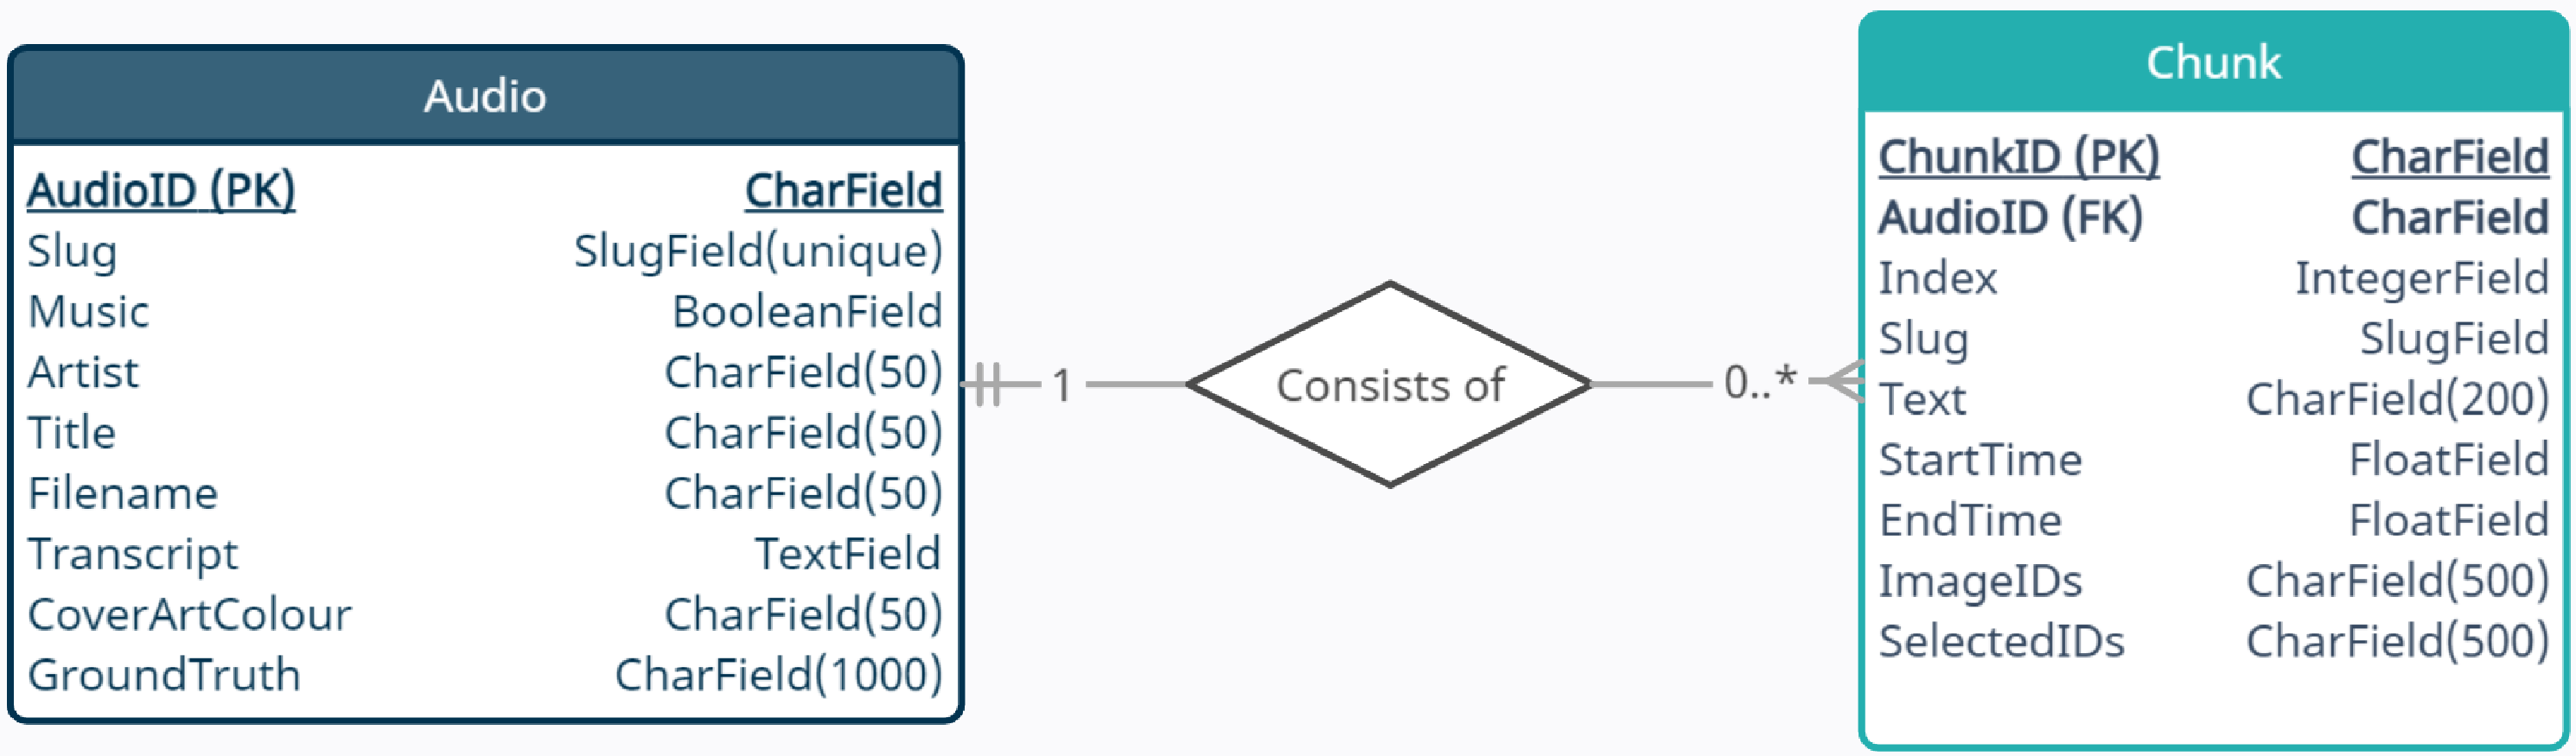
\includegraphics[width=1\textwidth]{figures/models_schema.pdf}
    \caption{An Entity Relation diagram showing the database schema made through Django models.}
    \label{fig:models_schema}
\end{figure}


\section{Program Structure}
All the main functionality is performed in the View component, represented by the file, \textbf{views.py}. However, each individual component outlined in the system architecture is abstracted into its own Python file in order to adhere to best software engineering practices. Each file, found in the \lstinline|utilities| folder, provide the required functions to accomplish a single task. This makes locating and adding functionality much easier compared to a disorganised program structure.

\subsection{Audio Retriever}
Represented in the \textbf{audio\_retriever.py} file, this component lends functions that will be used to extract the audio file from the user's submission on the Home page. Firstly, the \textbf{\lstinline|home|} view will clear the \lstinline|audio| and \lstinline|transcript| directories in order to save space. Next, the client's HTTP POST request will be analysed to extract the YouTube video URL or uploaded audio file. In the case of the YouTube video URL, the \textbf{\lstinline|download_yt|} function is called in order to isolate and download the audio from the video using the library pytube \citep{pytube}. This function also retrieves the English or Automated English captions, if present, as well as saving the thumbnail picture as the cover art. These can be pulled from the resulting \textbf{\lstinline|pytube.Youtube|} object. Alternatively, in the case of a file upload, the file will be validated if it's of an audio format and then saved into the \lstinline|audio| folder for further processing.


\subsection{Audio Recogniser}
Now that the audio source is saved within the \lstinline|audio| folder, it can be processed in order to identify its track title and artist name. It is initially assumed that it comprises of a music track. The \textbf{\lstinline|recognise_audio|} function attempts to match the audio source to a known music track using ShazamAPI \citep{shazamapi}. This API also provides the cover art URL for successful recognitions. This cover art is subsequently downloaded and saved within the \lstinline|coverart| folder using the HTTP Python library, Requests \citep{requests}. In addition to this, at later iterations, it was decided to use the primary colour of the cover art to further visually differentiate audio sources (Requirement \textbf{\#\ref{req:31}}). For this, the package, ColorThief \citep{colorthief}, was chosen to use image processing to identify the primary colour of the cover art which is then used to theme pages and links associated with the audio source.


\subsection{Synced Transcription Retriever}
This component holds multiple strategies to obtain a synced transcription of the audio in the LyRiCs (LRC) file format \citep{lrc}. The first method is retrieving the synced lyrics from the \cite{musixmatch} platform which holds an extensive database of song lyrics that are aligned with the song itself. The database is queried using the identified song title and artist name. If successful, the lyrics are saved within the \lstinline|transcript| folder, as well as the external database within the Audio model. Evidently, this method only works with music tracks, hence, this component also provides the capability of robust audio-to-text transcription, leveraging OpenAI's Whisper model \citep{whisper}. Due to memory limitations, only the \emph{'small'} model is loaded which was found to frequently misidentify words, hence its last resort status.  The resulting transcription is then formatted into the required LRC format.

This is the last processing step within the \textbf{\lstinline|home|} view which will conclude by instantiating a new Audio object using the obtained information. For non-music sources, the title field is filled in with the YouTube video title or uploaded file name. While the artist field is the video creator or simply left as empty for uploaded files. Finally, the user is redirected to the Audio page handled by the \textbf{\lstinline|audio|} view.

The \textbf{\lstinline|audio|} view divides the transcript using the phrase-level timings and initialises new Chunk objects for each segment denoted by new lines in the rendered Audio page. Each line is a clickable link to the corresponding Chunk page. For audio sources with no spoken language, no transcription is made and instead the user is appropriately notified in the rendered page.


\subsection{Image Retriever}
The \textbf{image\_retriever.py} file is responsible for image pre-processing and retrieval. In order to facilitate the freedom to configure the type of pre-trained CLIP model to use, a custom \textbf{\lstinline{CLIP}} class was made. This class holds properties such as the loaded model, tokenizer, and processor, as well as the file paths for all images and their corresponding embedding vectors. We chose the CLIP ViT-B/32 model for its moderate size for reasonable loading times and high performance. However, this model was trained with only English text and so to accommodate our requirement to support multiple languages (\textbf{\#\ref{req:12}}), we use a compatible Multilingual CLIP model that supports 100 languages: XLM-Roberta Large ViT-B/32 \citep{mclip}. Due to limited memory capacity, only one model can be loaded at one time so a Boolean flag is used to decide which model is loaded. Both models encode images and text into 512 dimensions of latent space and utilise the same vision transformer, meaning they can be interchanged according to the use case.

All images in the collection were pre-processed and embedded in batches using the pre-trained CLIP model and processor, to create a normalised NumPy matrix. This matrix was subsequently saved in a file so that it can be loaded into memory on application start-up. 

\label{sec:image_retriever:par:query_prompt}
The top 10 images are dynamically retrieved when a Chunk page is requested, handled by the \textbf{\lstinline{chunk}} view. The \textbf{\lstinline{query_prompt}} function takes in a text prompt, tokenizes it, and embeds it into the 512-dimensional feature space using the pre-loaded model and tokenizer. Following this, an exhaustive similarity search is performed, this involves calculating the cosine similarity between the embedded text vector with every image vector stored in the matrix. Since all vectors are normalised beforehand by their Euclidean (L2) norm as demonstrated in Equation \ref{eq:euclidean_normalisation}, the cosine similarity score is simply the dot product between the vectors, accomplished with \textbf{\lstinline{numpy.dot(text_emb, image_embs.T)}}. Listing \ref{lst:query_prompt} provides a code snippet implementing this process.

\begin{equation}
\begin{split}
    \text{normalise}&(\vec{x}) = \frac{\vec{x}}{\norm{\vec{x}}_2} \\
    \norm{\vec{x}}_2 = \sqrt{\sum_{i=1}^N \abs{x_i}^2} =& \sqrt{x_1^2 + x_2^2 + ... + x_N^2}
    \label{eq:euclidean_normalisation}
\end{split}
\end{equation}

\begin{lstlisting}[language=python, float, caption={An algorithm implementing the \textbf{\lstinline|query_prompt|} function that performs an exhaustive inner product search and retrieval of the top-$k$ images for the passed in text prompt. Defined as an internal function within the custom \textbf{\lstinline|CLIP|} class.}, label=lst:query_prompt]
    class CLIP:
    ...
        def query_prompt(self, prompt, k=10):
            # Tokenize and embed the text prompt using the CLIP model
            inputs = self.tokeniser(prompt, return_tensors="pt").to(self.device)
            text_embedding = self.model.get_text_features(**inputs).cpu().detach().numpy()
            # Normalise embedding with the Euclidean (L2) Norm
            text_embedding = text_embedding / np.linalg.norm(text_embedding)

            # Compute cosine similarity scores between prompt text and images
            scores = np.dot(text_embedding, self.image_vectors.T)
            # Sort in descending order and cut-off top-k
            top_k = np.argsort(-scores[0])[:k]

            return top_k
    ...
\end{lstlisting}

% \begin{equation}
% \begin{split}
%     \textbf{\lstinline|cos_sim|}(\vec{t}, \mathbf{I}) &= \vec{t} \cdot \mathbf{I}^T = 
%     \begin{bmatrix}
%         t_1  & t_2 & \cdots & t_N
%     \end{bmatrix}
%     \begin{bmatrix}
%         i_{11} & i_{12} & \cdots & i_{1N} \\
%         i_{21} & i_{22} & \cdots & i_{2N} \\
%         \vdots & \vdots & \ddots & \vdots \\
%         i_{M1} & i_{M2} & \cdots & i_{MN}
%     \end{bmatrix}^T \\
%     &=
%     \begin{bmatrix}
%         \left( \sum_{j=1}^N t_ji_{1j} \right) & \left( \sum_{j=1}^N t_ji_{2j} \right) & \cdots & \left( \sum_{j=1}^N t_ji_{Mj} \right)
%     \end{bmatrix}
%     \label{eq:dot_product}
% \end{split}
% \end{equation}

These similarity scores are subsequently sorted in descending order to get the 10 images that scored the highest with the text query which is then listed to the user on the Chunk page. In order to save unnecessary computation, these image indices are saved in the database associated with the Chunk object.


\subsection{Ground-Truth Builder}
Following the wireframes laid out during the design, the annotator can click on the 'Build Ground Truth' button on the Audio page and is, thereafter, transported to the first Chunk page to begin the relevance assessment exercise. As explained in \ref{sec:image_retriever:par:query_prompt}, the \textbf{\lstinline|query_prompt|} function will be called on an ad-hoc basis for each chunk in order to display the highest-scoring images. The annotator can then label the most fitting images by placing a check mark to denote relevance. This application uses the jQuery plugin, imgCheckbox \citep{imgcheckbox}, to dynamically inject checkboxes onto HTML \textbf{\lstinline|<img>|} tags on the webpage. 

All annotated images are saved within the Chunk object when the user submits an HTTP POST request which can occur when the 'Previous' or 'Next' buttons are pressed. This allows previously annotated Chunks to be viewed and amended fulfilling requirement \textbf{\#\ref{req:11}}. Additionally, throughout testing it was found to be burdensome to annotate chunks with repeating textual content, leading to the addition of requirement \textbf{\#\ref{req:16}}. This feature greatly reduced annotation effort and efficiency since all duplicate chunks can be updated at once and skipped during relevance assessment.

The full ground-truth can only be viewed when the user clicks the 'Finish' button on the last chunk of the transcript. The ground-truth is built chunk by chunk, appending to a Python dictionary storing relevant information of the audio source and chunks. The indices of the assessed images are stored here as well as their corresponding file paths in order to ease exporting. In order to release the data in a human-readable and easily accessible format (\textbf{\#\ref{req:9}}), the resulting Python dictionary is serialised into JavaScript Object Notation (JSON) \citep{json}. This is an open standard format that is language-independent. A preview of the data is subsequently rendered in the Ground-Truth page with a clear button to download it.

\subsubsection{Determining Pooling Depth}
\label{sec:determining_pool_depth}
The final pooling depth of $k=10$ was determined through trial and error since it was difficult to estimate the effectiveness of CLIP models on multi-conceptual text prompts that are so common in spoken language, especially song lyrics. Retrieving the top-10 images was determined to be the ideal depth that is able to fit in one page without excessive rescaling as well as not increasing relevance assessment effort. However, it was noticed that in rare occasions of extreme ambiguity of text, more images were required to be assessed to find any relevance. This was also picked up during user evaluations in \ref{sec:usability_testing} where it may be beneficial to increase $k$ for very abstract ideas.


\subsection{Video Compiler}
The video compiler component implemented in the \textbf{videography.py} file, takes care of generating the video primarily using the library MoviePy \citep{moviepy}. The video is built incrementally, much like the ground-truth construction, by selecting the top-1 image for each chunk and concatenating \textbf{\lstinline|ImageClip|s} in sequence. Their durations are simply the difference between the chunk start and end times. \textbf{\lstinline|TextClip|s} showing the chunk text are placed below corresponding images. Black \textbf{\lstinline|ColorClip|s} are used to fill parts of the audio lacking spoken words. Lastly, the audio source is added to the final \textbf{\lstinline|VideoClip|} which is then written into an MP4 file in the \lstinline|video| folder. This file is then embedded into the HTML of the Video page for the user to subsequently play and download.


\section{Summary}
This chapter described the steps taken in manifesting the blueprint designs into a concrete product. Key implementation details were explained as well as the challenges faced along the development process. The rationale for the chosen language and web framework was given, in addition to how the various libraries are integrated into the project in order to reduce the complexity of the project's development. A full account of the program's structure and technical accomplishments were also provided. A walkthrough of the implemented application is provided in Appendix \ref{app:walkthrough}. Now that the application has been fully implemented, it presents an opportunity to assess its efficacy in achieving the project's original goals. 

% What did you do to implement this idea, and what technical achievements did you make?
% \section{Guidance}
% You can't talk about everything. Cover the high level first, then cover important, relevant or impressive details.

% \section{General guidance for technical writing}

% These points apply to the whole dissertation, not just this chapter.

% \subsection{Figures}
% \emph{Always} refer to figures included, like Figure \ref{fig:relu}, in the body of the text. Include full, explanatory captions and make sure the figures look good on the page.
% You may include multiple figures in one float, as in Figure \ref{fig:synthetic}, using \texttt{subcaption}, which is enabled in the template.


% % Figures are important. Use them well.
% \begin{figure}[htb]
%     \centering
%     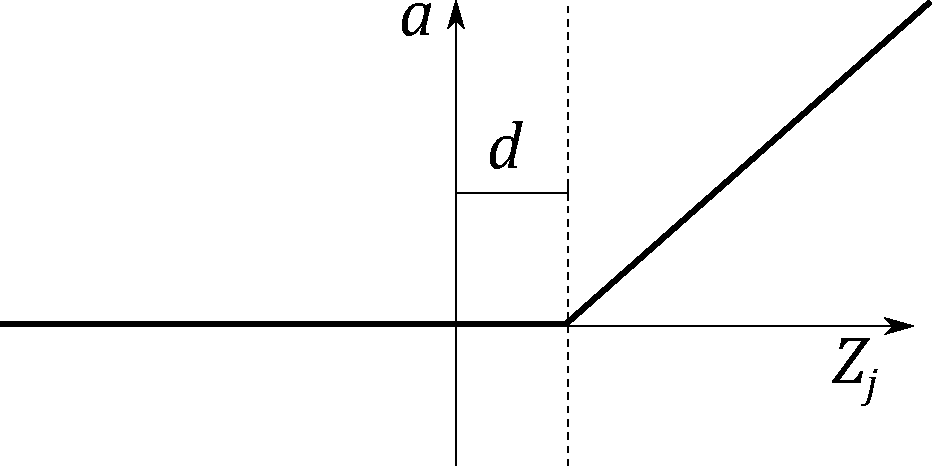
\includegraphics[width=0.5\linewidth]{figures/relu.pdf}    

%     \caption{In figure captions, explain what the reader is looking at: ``A schematic of the rectifying linear unit, where $a$ is the output amplitude,
%     $d$ is a configurable dead-zone, and $Z_j$ is the input signal'', as well as why the reader is looking at this: 
%     ``It is notable that there is no activation \emph{at all} below 0, which explains our initial results.'' 
%     \textbf{Use vector image formats (.pdf) where possible}. Size figures appropriately, and do not make them over-large or too small to read.
%     }

%     % use the notation fig:name to cross reference a figure
%     \label{fig:relu} 
% \end{figure}


% \begin{figure}[htb] 
%     \centering
%     \begin{subfigure}[b]{0.45\textwidth}
%         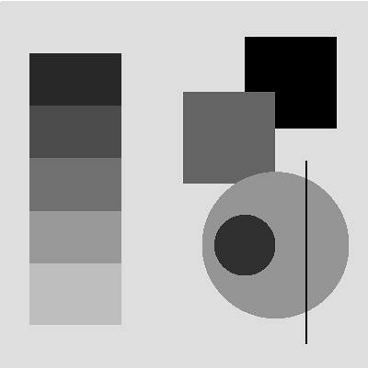
\includegraphics[width=\textwidth]{figures/synthetic.png}
%         \caption{Synthetic image, black on white.}
%         \label{fig:syn1}
%     \end{subfigure}
%     ~ %add desired spacing between images, e. g. ~, \quad, \qquad, \hfill etc. 
%       %(or a blank line to force the subfigure onto a new line)
%     \begin{subfigure}[b]{0.45\textwidth}
%         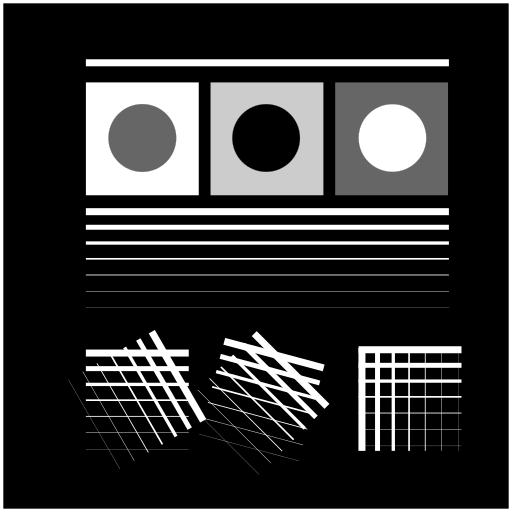
\includegraphics[width=\textwidth]{figures/synthetic_2.png}
%         \caption{Synthetic image, white on black.}
%         \label{fig:syn2}
%     \end{subfigure}
%     ~ %add desired spacing between images, e. g. ~, \quad, \qquad, \hfill etc. 
%     %(or a blank line to force the subfigure onto a new line)    
%     \caption{Synthetic test images for edge detection algorithms. \subref{fig:syn1} shows various gray levels that require an adaptive algorithm. \subref{fig:syn2}
%     shows more challenging edge detection tests that have crossing lines. Fusing these into full segments typically requires algorithms like the Hough transform.
%     This is an example of using subfigures, with \texttt{subref}s in the caption.
%     }\label{fig:synthetic}
% \end{figure}

% \clearpage

% \subsection{Equations}

% Equations should be typeset correctly and precisely. Make sure you get parenthesis sizing correct, and punctuate equations correctly 
% (the comma is important and goes \textit{inside} the equation block). Explain any symbols used clearly if not defined earlier. 

% For example, we might define:
% \begin{equation}
%     \hat{f}(\xi) = \frac{1}{2}\left[ \int_{-\infty}^{\infty} f(x) e^{2\pi i x \xi} \right],
% \end{equation}    
% where $\hat{f}(\xi)$ is the Fourier transform of the time domain signal $f(x)$.

% \subsection{Algorithms}
% Algorithms can be set using \texttt{algorithm2e}, as in Algorithm \ref{alg:metropolis}.

% % NOTE: line ends are denoted by \; in algorithm2e
% \begin{algorithm}
%     \DontPrintSemicolon
%     \KwData{$f_X(x)$, a probability density function returing the density at $x$.\; $\sigma$ a standard deviation specifying the spread of the proposal distribution.\;
%     $x_0$, an initial starting condition.}
%     \KwResult{$s=[x_1, x_2, \dots, x_n]$, $n$ samples approximately drawn from a distribution with PDF $f_X(x)$.}
%     \Begin{
%         $s \longleftarrow []$\;
%         $p \longleftarrow f_X(x)$\;
%         $i \longleftarrow 0$\;
%         \While{$i < n$}
%         {
%             $x^\prime \longleftarrow \mathcal{N}(x, \sigma^2)$\;
%             $p^\prime \longleftarrow f_X(x^\prime)$\;
%             $a \longleftarrow \frac{p^\prime}{p}$\;
%             $r \longleftarrow U(0,1)$\;
%             \If{$r<a$}
%             {
%                 $x \longleftarrow x^\prime$\;
%                 $p \longleftarrow f_X(x)$\;
%                 $i \longleftarrow i+1$\;
%                 append $x$ to $s$\;
%             }
%         }
%     }
    
% \caption{The Metropolis-Hastings MCMC algorithm for drawing samples from arbitrary probability distributions, 
% specialised for normal proposal distributions $q(x^\prime|x) = \mathcal{N}(x, \sigma^2)$. The symmetry of the normal distribution means the acceptance rule takes the simplified form.}\label{alg:metropolis}
% \end{algorithm}

% \subsection{Tables}

% If you need to include tables, like Table \ref{tab:operators}, use a tool like https://www.tablesgenerator.com/ to generate the table as it is
% extremely tedious otherwise. 

% \begin{table}[]
%     \caption{The standard table of operators in Python, along with their functional equivalents from the \texttt{operator} package. Note that table
%     captions go above the table, not below. Do not add additional rules/lines to tables. }\label{tab:operators}
%     %\tt 
%     \rowcolors{2}{}{gray!3}
%     \begin{tabular}{@{}lll@{}}
%     %\toprule
%     \textbf{Operation}    & \textbf{Syntax}                & \textbf{Function}                            \\ %\midrule % optional rule for header
%     Addition              & \texttt{a + b}                          & \texttt{add(a, b)}                                    \\
%     Concatenation         & \texttt{seq1 + seq2}                    & \texttt{concat(seq1, seq2)}                           \\
%     Containment Test      & \texttt{obj in seq}                     & \texttt{contains(seq, obj)}                           \\
%     Division              & \texttt{a / b}                          & \texttt{div(a, b) }  \\
%     Division              & \texttt{a / b}                          & \texttt{truediv(a, b) } \\
%     Division              & \texttt{a // b}                         & \texttt{floordiv(a, b)}                               \\
%     Bitwise And           & \texttt{a \& b}                         & \texttt{and\_(a, b)}                                  \\
%     Bitwise Exclusive Or  & \texttt{a \textasciicircum b}           & \texttt{xor(a, b)}                                    \\
%     Bitwise Inversion     & \texttt{$\sim$a}                        & \texttt{invert(a)}                                    \\
%     Bitwise Or            & \texttt{a | b}                          & \texttt{or\_(a, b)}                                   \\
%     Exponentiation        & \texttt{a ** b}                         & \texttt{pow(a, b)}                                    \\
%     Identity              & \texttt{a is b}                         & \texttt{is\_(a, b)}                                   \\
%     Identity              & \texttt{a is not b}                     & \texttt{is\_not(a, b)}                                \\
%     Indexed Assignment    & \texttt{obj{[}k{]} = v}                 & \texttt{setitem(obj, k, v)}                           \\
%     Indexed Deletion      & \texttt{del obj{[}k{]}}                 & \texttt{delitem(obj, k)}                              \\
%     Indexing              & \texttt{obj{[}k{]}}                     & \texttt{getitem(obj, k)}                              \\
%     Left Shift            & \texttt{a \textless{}\textless b}       & \texttt{lshift(a, b)}                                 \\
%     Modulo                & \texttt{a \% b}                         & \texttt{mod(a, b)}                                    \\
%     Multiplication        & \texttt{a * b}                          & \texttt{mul(a, b)}                                    \\
%     Negation (Arithmetic) & \texttt{- a}                            & \texttt{neg(a)}                                       \\
%     Negation (Logical)    & \texttt{not a}                          & \texttt{not\_(a)}                                     \\
%     Positive              & \texttt{+ a}                            & \texttt{pos(a)}                                       \\
%     Right Shift           & \texttt{a \textgreater{}\textgreater b} & \texttt{rshift(a, b)}                                 \\
%     Sequence Repetition   & \texttt{seq * i}                        & \texttt{repeat(seq, i)}                               \\
%     Slice Assignment      & \texttt{seq{[}i:j{]} = values}          & \texttt{setitem(seq, slice(i, j), values)}            \\
%     Slice Deletion        & \texttt{del seq{[}i:j{]}}               & \texttt{delitem(seq, slice(i, j))}                    \\
%     Slicing               & \texttt{seq{[}i:j{]}}                   & \texttt{getitem(seq, slice(i, j))}                    \\
%     String Formatting     & \texttt{s \% obj}                       & \texttt{mod(s, obj)}                                  \\
%     Subtraction           & \texttt{a - b}                          & \texttt{sub(a, b)}                                    \\
%     Truth Test            & \texttt{obj}                            & \texttt{truth(obj)}                                   \\
%     Ordering              & \texttt{a \textless b}                  & \texttt{lt(a, b)}                                     \\
%     Ordering              & \texttt{a \textless{}= b}               & \texttt{le(a, b)}                                     \\
%     % \bottomrule
%     \end{tabular}
%     \end{table}
% \subsection{Code}

% Avoid putting large blocks of code in the report (more than a page in one block, for example). Use syntax highlighting if possible, as in Listing \ref{lst:callahan}.

% \begin{lstlisting}[language=python, float, caption={The algorithm for packing the $3\times 3$ outer-totalistic binary CA successor rule into a 
%     $16\times 16\times 16\times 16$ 4 bit lookup table, running an equivalent, notionally 16-state $2\times 2$ CA.}, label=lst:callahan]
%     def create_callahan_table(rule="b3s23"):
%         """Generate the lookup table for the cells."""        
%         s_table = np.zeros((16, 16, 16, 16), dtype=np.uint8)
%         birth, survive = parse_rule(rule)

%         # generate all 16 bit strings
%         for iv in range(65536):
%             bv = [(iv >> z) & 1 for z in range(16)]
%             a, b, c, d, e, f, g, h, i, j, k, l, m, n, o, p = bv

%             # compute next state of the inner 2x2
%             nw = apply_rule(f, a, b, c, e, g, i, j, k)
%             ne = apply_rule(g, b, c, d, f, h, j, k, l)
%             sw = apply_rule(j, e, f, g, i, k, m, n, o)
%             se = apply_rule(k, f, g, h, j, l, n, o, p)

%             # compute the index of this 4x4
%             nw_code = a | (b << 1) | (e << 2) | (f << 3)
%             ne_code = c | (d << 1) | (g << 2) | (h << 3)
%             sw_code = i | (j << 1) | (m << 2) | (n << 3)
%             se_code = k | (l << 1) | (o << 2) | (p << 3)

%             # compute the state for the 2x2
%             next_code = nw | (ne << 1) | (sw << 2) | (se << 3)

%             # get the 4x4 index, and write into the table
%             s_table[nw_code, ne_code, sw_code, se_code] = next_code

%         return s_table

% \end{lstlisting}

%==================================================================================================
\chapter{Evaluation} 
This chapter serves to evaluate the fully implemented application by looking at how many of the requirements specified in Chapter \ref{chap:requirements} have been fulfilled. This chapter is split into two sections, the first part evaluates the implemented Automatic Videography tool by looking at ways to improve its efficiency, as well as comparing it against the system that came before. The latter half entails evaluating the usability of the relevance assessment interface.

Since this product's purpose is to aid users in their creative pursuits and the assembly of test collections, rather than addressing a quantifiable problem, some requirements pose a greater challenge for evaluation. Non-functional requirements are particularly challenging because, unlike functional requirements which can be either implemented or not, non-functional requirements are more subjective in nature. A number of experiments must be conducted in order to gather empirical measures that can help answer this question. Nevertheless, it is inevitable that some level of interpretation will be necessary, but efforts will be made to approach the highest degree of objectivity.

\section{Automatic Videography}
\subsection{Improving Retrieval Efficiency with FAISS}
The retrieval system involves meticulous similarity search and sort operations which pose serious scalability issues. Expanding to larger image collections or running multiple videography pipelines at once is currently impractical. Therefore more efficient strategies for retrieving the images were analysed including Facebook's AI Similarity Search (FAISS) \citep{johnson2019faiss}. This library offers a range of efficient indexing strategies for fast similarity searching, with the key idea of clustering similar documents into identical cells. In our case, it was necessary to utilise the inner product indexing technique, \textbf{\lstinline|faiss.IndexFlatIP|}, to match CLIP's training procedure. This path ultimately lead to a dead end due to a huge decline in retrieval accuracy, even with the remarkable 98\% decrease in the mean search time compared to an exhaustive search. 

Experiments were conducted to evaluate different parameter tunings for the inverted file index with a Product Quantizer encoding, \textbf{\lstinline|faiss.IndexIVFPQ|}. Each configuration was then compared with the original flat indexing strategy, i.e. exhaustive searching. The indexed collections were tested on a set of 10 audio sources which provided a total of 399 phrase-level text prompts. Three sets of values were used for the \textbf{\lstinline|nlist|} parameter namely: 2048, 4096 and $16\,384$. These values determine the number of Voronoi cells to partition the index of image vectors. It is common to pick a value that is a power of 2 that is close to $4\sqrt{M}$, where $M$ is the total number of document vectors \citep{milvus_nlist}. Our filtered static collection consists of $1\,281\,121$ images resulting in a recommended value that is close to the second test value. 

\begin{table}
    \centering
    \begin{tabular}{|c|c|c|}
        \hline
        \textbf{Indexing Method} & \textbf{Mean Retrieval Time (s)} & \textbf{Mean Jaccard Similarity} \\
        \hline
        \hline
        Flat (Exhaustive) & 0.2833 & - \\
        \hline
        IndexIVFPQ (\emph{\lstinline|nlist|=2048}) & 0.0024 & 0.0 \\
        \hline
        IndexIVFPQ (\emph{\lstinline|nlist|=4096}) & 0.0035 & 0.0 \\
        \hline
        IndexIVFPQ (\emph{\lstinline|nlist|=16384}) & 0.0094 & 0.0 \\
        \hline
    \end{tabular}
    
    \caption{ The results of the FAISS experiment to find the best indexing configuration to expedite the search and retrieval process. The experiment was tested on $399$ text prompts extracted from $10$ audio sources. The mean time to retrieve the top ten images from a text prompt is shown for each strategy as well as the mean Jaccard similarity of the retrievals against the original Flat index method. All retrievals were performed using an \lstinline|nprobe| $=20$.}
    \label{tab:faiss_experiment}
\end{table}

Table \ref{tab:faiss_experiment} outlines the results of the experiment including the mean retrieval times to obtain the top 10 images for all 399 text queries. The mean Jaccard similarities shown was used to determine the accuracy of the retrievals by measuring the overlaps against the original exhaustive approach. From the results, it is evident that while the configurations are able to retrieve images over 30 times faster, they achieved a 0\% accuracy within the top ten images. This elicited inspecting the quality of images retrieved by the different FAISS systems revealing some degree of relevance. Although, in many instances, the retrieved images did not pertain to the given prompt. Figure \ref{fig:faiss_retrieval_comp} illustrates a particular comparison for the text query, \emph{"play it on repeat"}. We believe more work is required to enhance the scalability of this project's videography system, which can be achieved by experimenting with alternate FAISS indexing strategies.

\begin{figure}[htb]
    \centering
    \begin{subfigure}[b]{1\textwidth}
        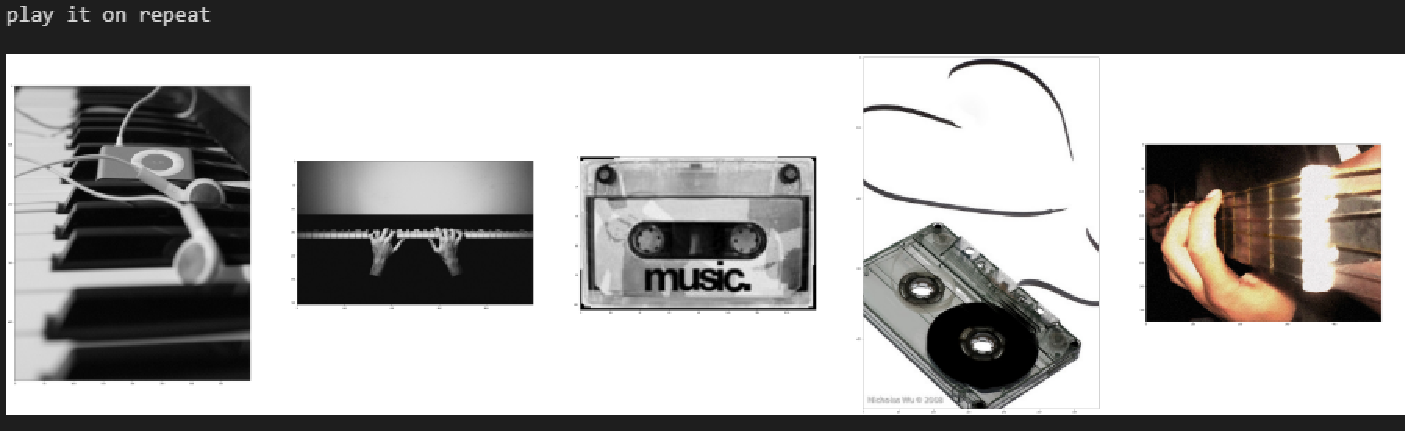
\includegraphics[width=\textwidth]{figures/exhaustive_retrievals.pdf}
        \caption{Original Flat Index (i.e. exhaustive search)}
        \label{fig:exhaustive_retrievals}
    \end{subfigure} \\
    ~ 
    \par\medskip
    \begin{subfigure}[b]{1\textwidth}
        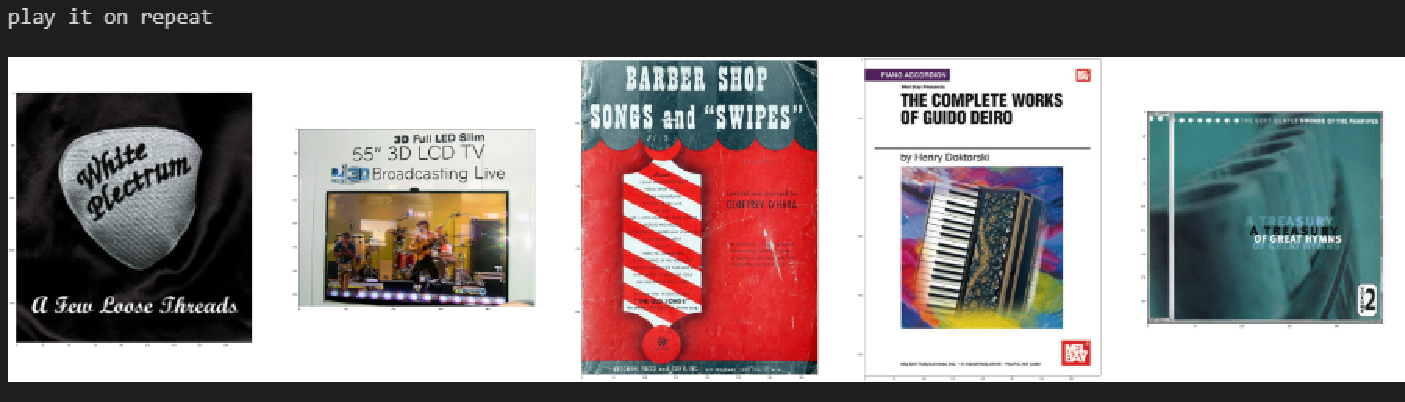
\includegraphics[width=\textwidth]{figures/faiss_retrievals.pdf}
        \caption{FAISS IndexIVFPQ (\lstinline|nlist|=16384) configuration}
        \label{fig:faiss_retrievals}
    \end{subfigure}
    ~    
    \caption{The top five images retrieved by both configurations, ordered by their similarity score to the text query: "play it on repeat".}
    \label{fig:faiss_retrieval_comp}
\end{figure}


\subsection{Video Generation Time Testing}
\label{sec:video_generation_time}
Despite the unsuccessful efforts in improving retrieval speeds with FAISS, one of the objectives of this project was to improve the slow video generation times of the previous system. This led to non-functional requirement \textbf{\#\ref{req:26}}:

\begin{itemize}
    \item \textbf{Should Have:} The videos being generated in a more reasonable amount of time than the prior system.
\end{itemize}

In order to check if this requirement has been satisfied, experiments must be conducted in order to find and compare the average time taken to generate a video using both systems. This experiment was run with 20 audio sources each of varying lengths, averaging around 3 minutes and 20 seconds (Standard Deviation: $\sigma = 0.84$ min). The mean number of phrase-level chunks present per source was 47.9 ($\sigma = 18.4$ chunks) with an overall total of 958 chunks and images being retrieved during the experiment. Before conducting the experiment, it was postulated that the time taken to compile a video is determined on the number of MoviePy video clips needed. As made evident by Figure \ref{fig:videography_against_wchunks}, this is generally the case as the video compilation time is dependant on \textbf{both} the number of phrase-level chunks present and the audio length.

\begin{figure}[H]
    \centering
    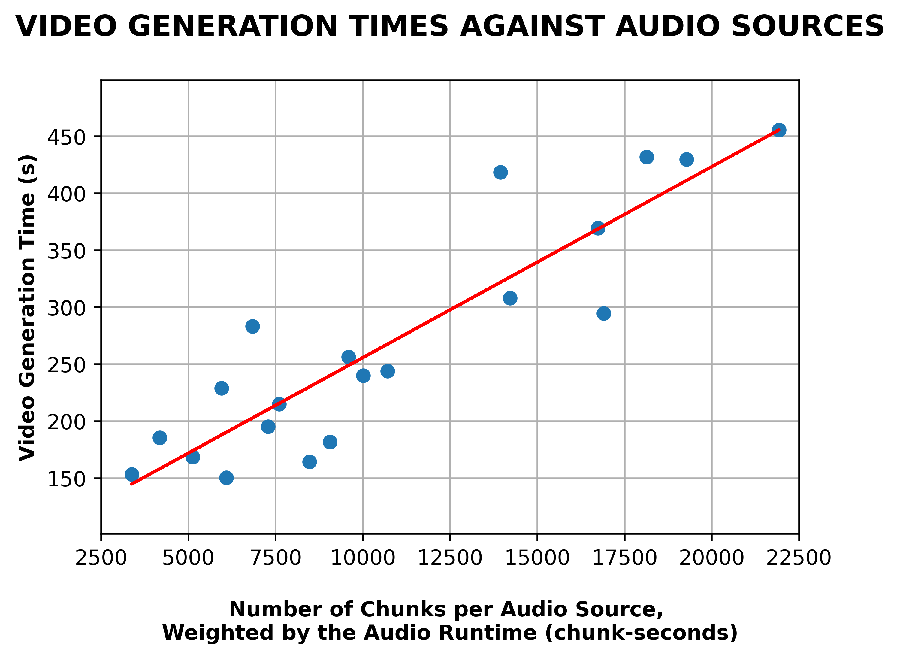
\includegraphics[width=0.76\textwidth]{figures/video_generation_against_wchunks.pdf}
    \caption{Graph showing the general relationship between the video generation time, and the number of chunks present in audio sources, weighted by the audio runtime. The data was plotted from the video generation times of the current system on 20 distinct audio sources.}
    \label{fig:videography_against_wchunks}
\end{figure}

This is because the clips can comprise \textbf{\lstinline|ImageClip|s} and \textbf{\lstinline|TextClip|s}, which is determined by the number of chunks present. In addition, \textbf{\lstinline|ColorClip|s} are used to fill gaps between chunks meaning this is influenced by the audio duration. Therefore, in order to minimise the effect of both the number of chunks and the audio runtime, a diverse range of sources were picked that are representative of the tool's use case. 

Table \ref{tab:videography_times} in the Appendix lists the resulting video generation times for all 20 sources on both the previous and current systems. A summary is shown in the form of box plots in Figure \ref{fig:videography_timed}. As illustrated, the current system generates videos
42\% faster than the previous system on average. The current system achieved a mean video generation time of 4 minutes 29 seconds ($\sigma = 1.65$ min), while the latter, 7 minutes 44 seconds ($\sigma = 2.63$ min). It is interesting to note that the prior system's times vary a lot more. This is most likely due to the fact that it necessitated downloading images from Google's image catalogue, resulting in its retrieval time being subject to unstable internet speeds. In contrast, this system has the benefit of retrieving from a locally stored collection.

In summary, the experiment results empirically show that the non-functional requirement \textbf{\#\ref{req:26}} has been successfully fulfilled. Considering that this system elevates video compilation complexity by including \textbf{\lstinline|TextClip|s}, something that was absent from the preceding system, the results are promising. However, this can be further improved by using a more intelligent indexing strategy using resources such as FAISS, which offers faster similarity search times than the current exhaustive approach.

\begin{figure}
    \centering
    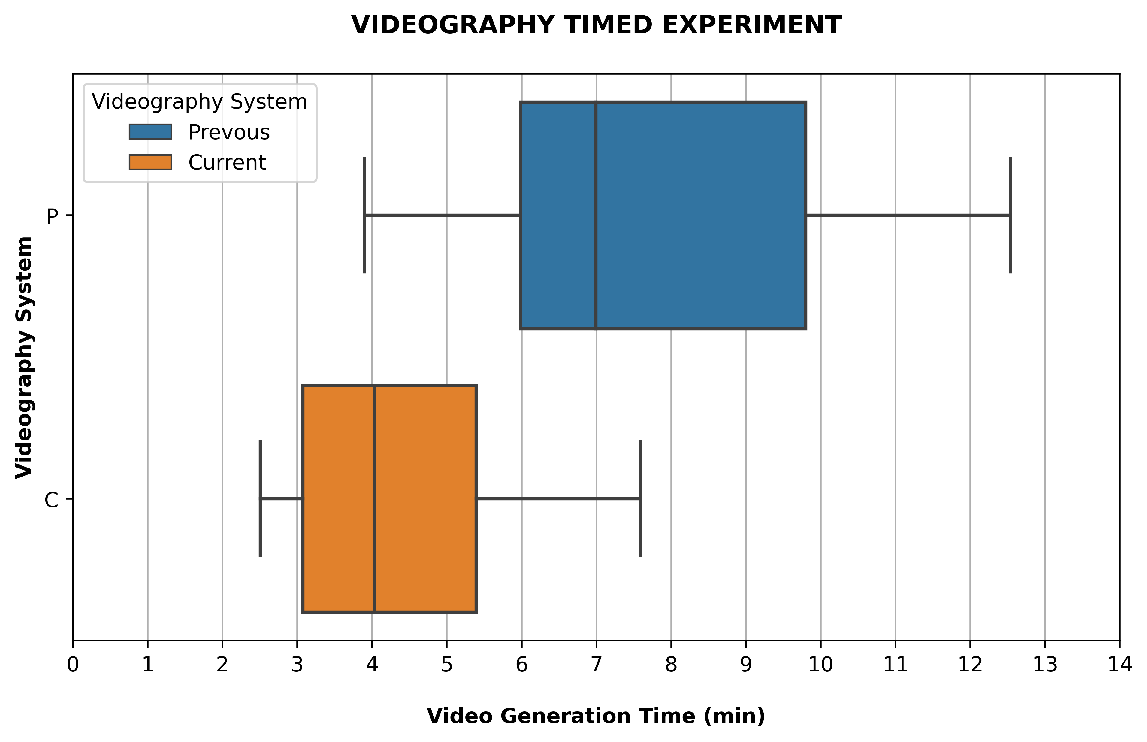
\includegraphics[width=1\textwidth]{figures/videography_timed_experiment.pdf}
    \caption{Box plot showing a comparative summary of the video generation times for both the preceding and current videography systems, tested on 20 distinct audio sources. The Caption Extraction method used was throughout the experiment for the prior system.}
    \label{fig:videography_timed}
\end{figure}


\subsection{Video Quality Testing}
Another requirement of the project was \textbf{\#\ref{req:27}}:

\begin{itemize}
    \item \textbf{Should Have:} The generated video having a higher resolution than the prior system.
\end{itemize}

The previous system restricted the resolution of images to 200 by 100 pixels due to the high disparity of image sizes downloaded from Google. This was found to cause frequent incompatibility issues with MoviePy's video compilation algorithm. This resulted in numerous complaints about breaking immersion during its user evaluation phase. To address this issue, a potential solution is to minimise this disparity by filtering images with outlier resolutions from the dataset. Fortunately, the ImageNet-1k dataset, which this project employs, already addresses this concern by providing images with consistent resolutions to streamline machine learning tasks. Experiments conducted identified that the images stored in the collection had a mean resolution of $473.0 \times 405.5$ with a standard deviation of 208.1 pixels for width and 178.7 pixels for height. Therefore, the quality of videos did not become a burden during this project. Figure \ref{fig:video_quality_comp} shows a comparison of the quality of compiled videos for \emph{America}'s song, \emph{"A Horse With No Name"}, demonstrating that this requirement has been fulfilled.

\begin{figure}
    \centering
    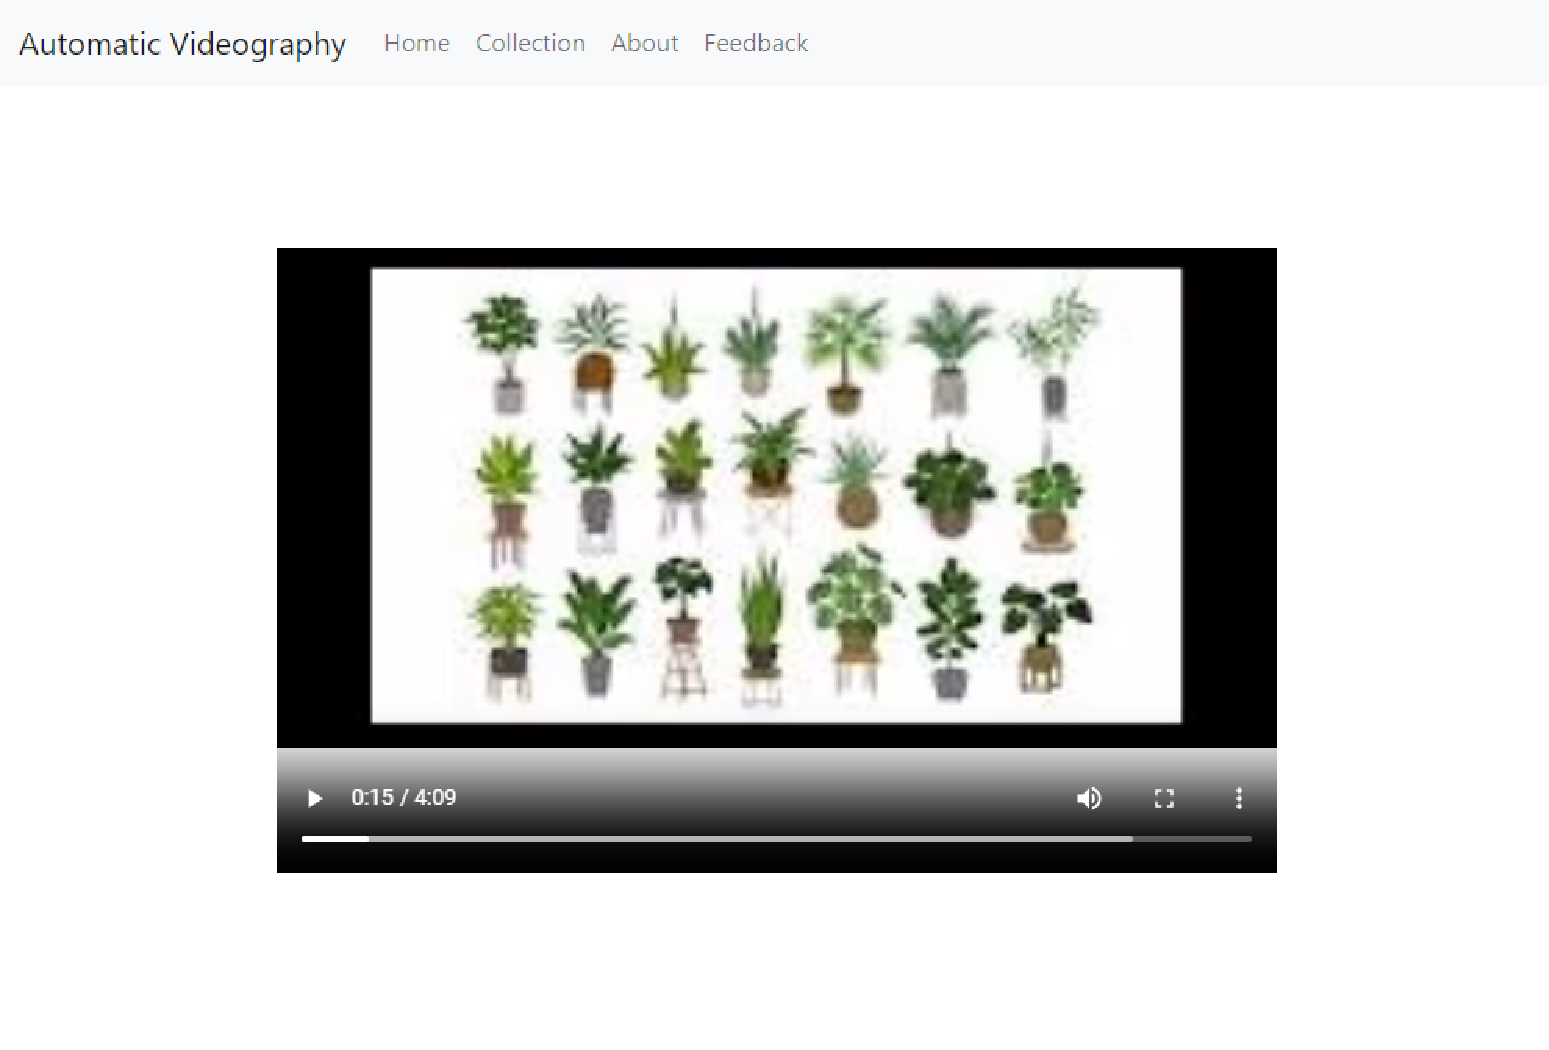
\includegraphics[width=0.5\textwidth]{figures/ahwnn_quality_p.pdf}
    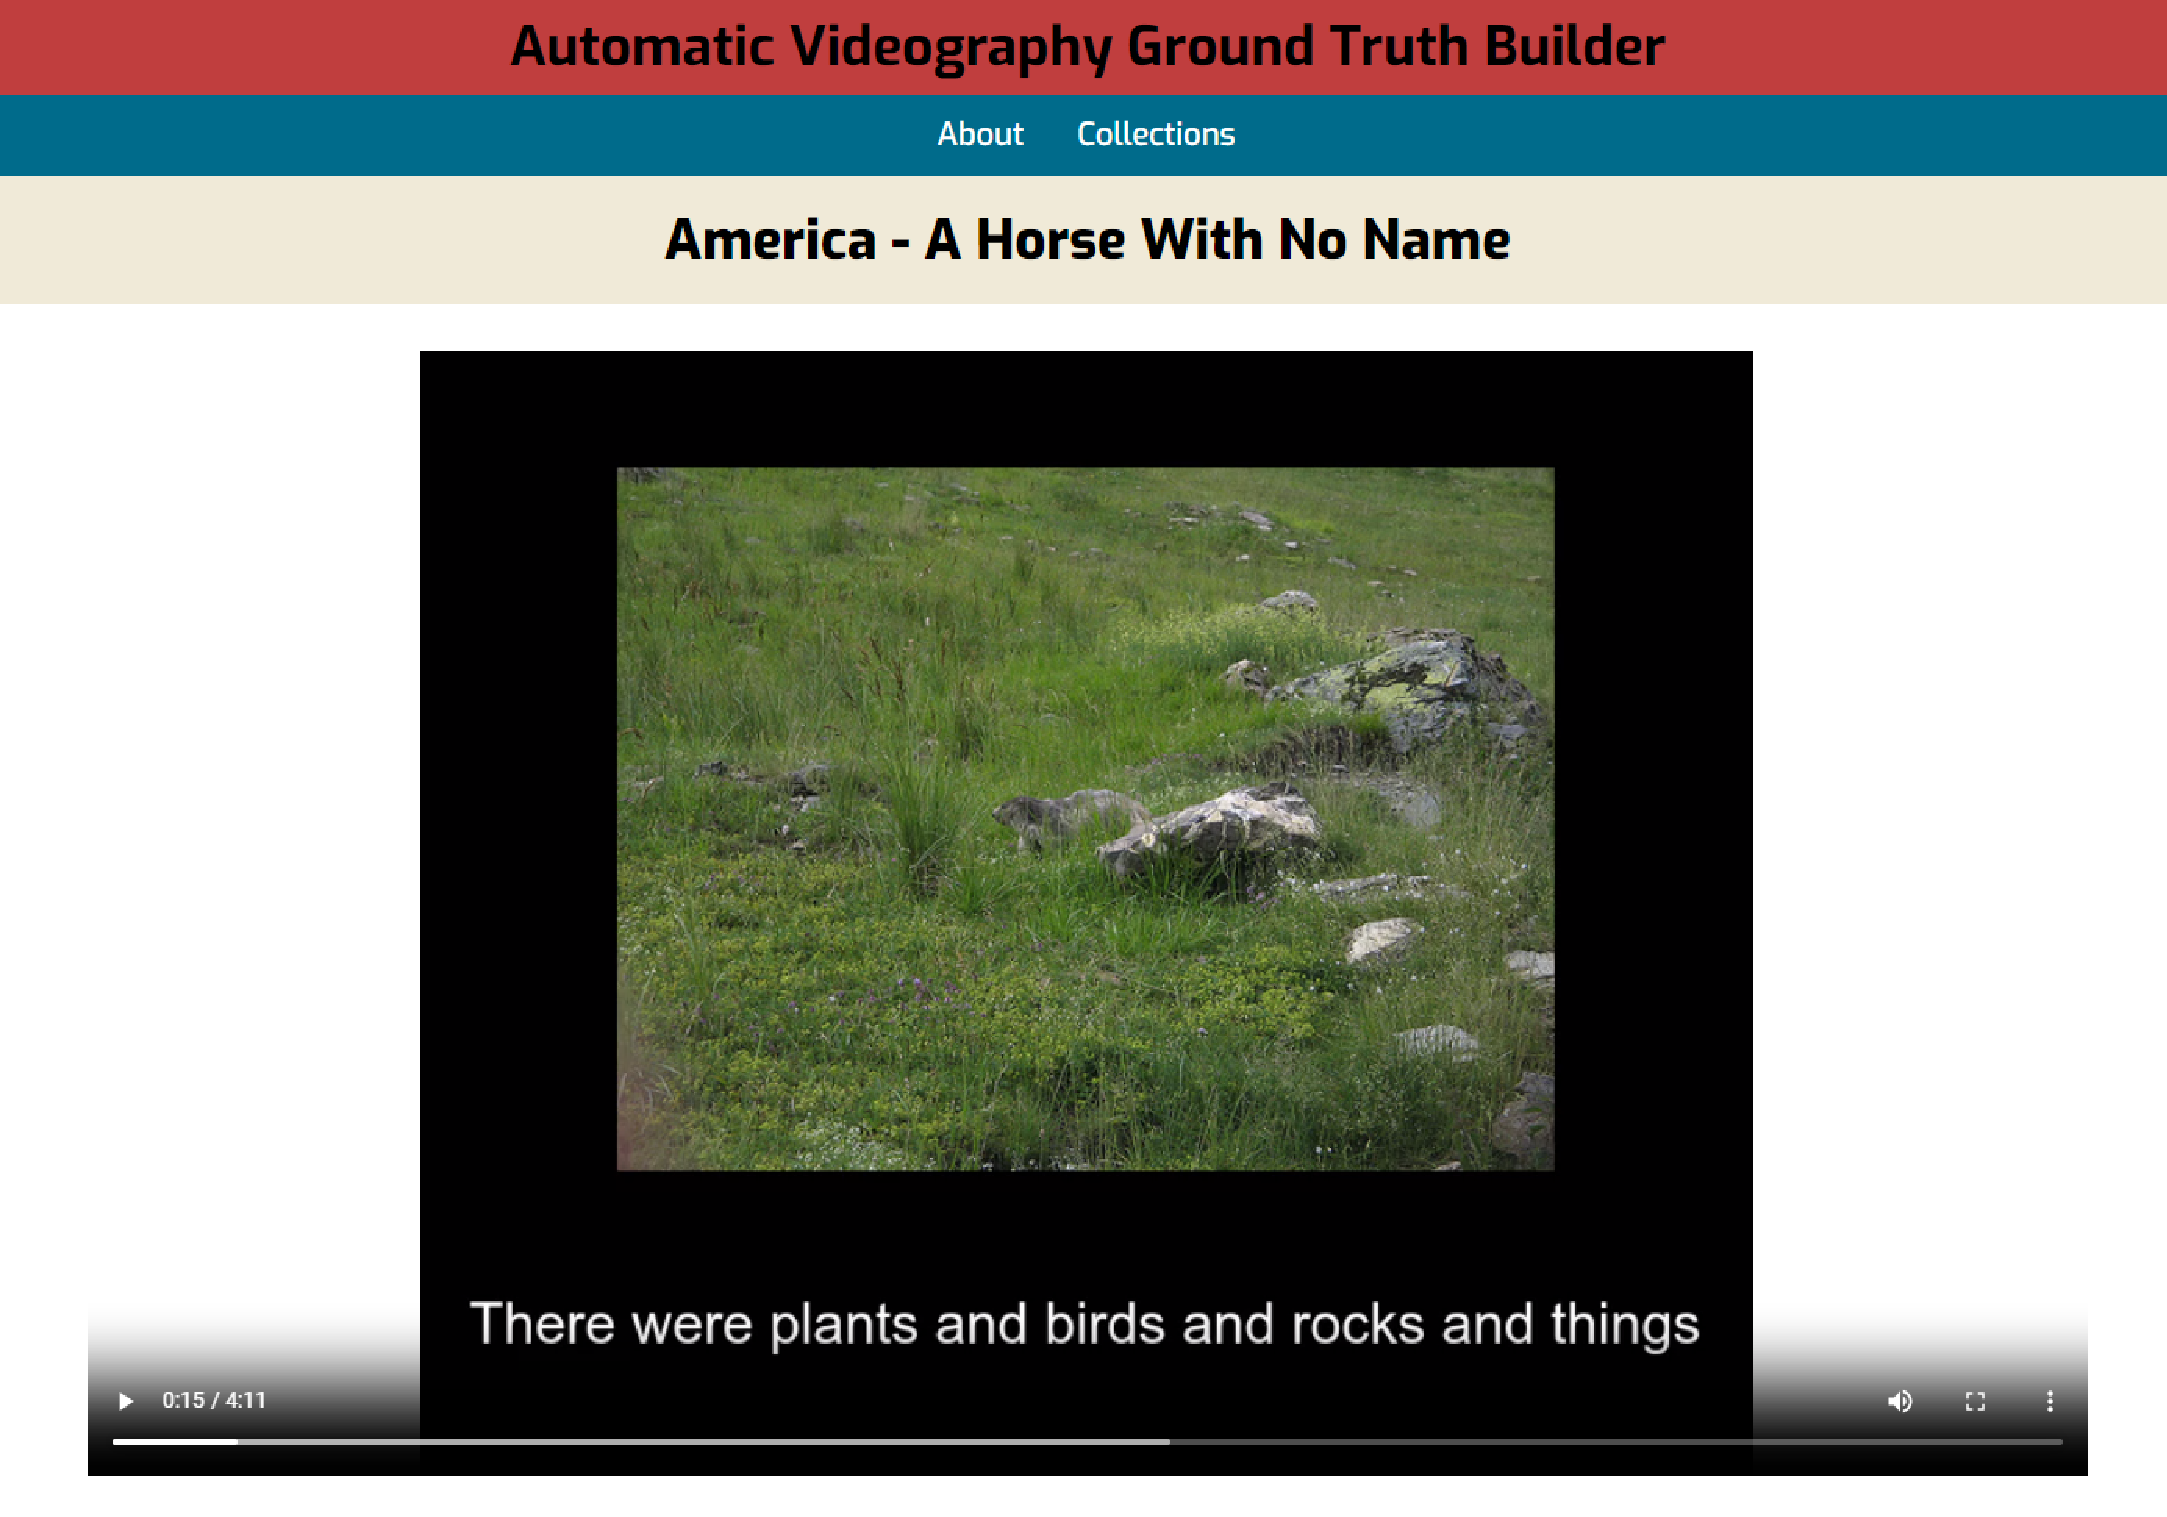
\includegraphics[width=0.49\textwidth]{figures/ahwnn_quality_c.pdf}
    \caption{Comparison of the quality of videos generated by the preceding (left) and new (right) videography systems. The videos were screenshotted at the same timestamp in order to show a fair comparison of the same segment within the song "A Horse With No Name" by America.}
    \label{fig:video_quality_comp}
\end{figure}


\section{Ground-Truth Annotation Interface}
\subsection{Usability Testing}
\label{sec:usability_testing}
This project aimed to produce an interface that eases the relevance assessment of images from text for videography tasks. Hence, one of the conditions set forth was that the interface needed to be user-friendly enough for any user to carry out a relevance assessment on a specified audio source. To test this non-functional requirement \textbf{\#\ref{req:20}}:

\begin{itemize}
    \item \textbf{Should Have:} The application having a presentable user interface that is easy for any user to understand and learn quickly.
\end{itemize}

A usability survey must be conducted with a diverse set of users that is representative of the target demographic. 16 participants took part in the user study, where they were each given a single task to complete using the developed web application. The study complied with the Ethics Checklist outlined by the School of Computing Science as all data collected was anonymised and no personal data was collected. A signed copy of this checklist can be found in Appendix \ref{app:ethics_checklist}.

A template of the briefing form given to each participant can be found in Appendix \ref{app:usability_eval_brief}. In summary, each participant was given an audio source picked from a predefined list of music tracks and educational videos on YouTube. The participant was then expected to find and input the required information in order to start constructing a ground-truth using the application. As the study was focused on evaluating the interface's usability, participants had to rely solely on the information presented to navigate the website, as no explicit instructions were given on how to complete the task. All participants were given a maximum of 10 minutes, however, it was not expected for them to complete the ground-truth for the full audio. This was due to the varying lengths and the number of chunks present in the sources. Nonetheless, from prior testing, it was expected that most participants could complete 85-90\% of the ground-truth for audio sources averaging around 50-55 chunks.

\subsubsection{Usability Rating}
Once the participants finished their allotted tasks, they were asked to complete a survey asking questions about their experience with the interface. A copy of the survey form is provided in Appendix \ref{app:usability_survey}. The first question asked participants to rate the interface design's overall intuitiveness on a scale of 1 to 5. The higher the rating, the higher they found the application easy to navigate through. On average, the usability of the site was rated 4.4 out of 5 by the participants, with a standard deviation of 0.5. This is because all participants chose either 4 or 5, as illustrated in Figure \ref{fig:rating_distribution}. While this score shows promise, it is not sufficient to completely check off our criterion. Therefore, the remainder of the survey comprised of open-ended questions. These aimed to obtain precise details about the participants' preferences and dislikes regarding the application. Moreover, the open-ended questions enabled respondents to suggest additional features that could potentially enhance the application in future iterations.

\begin{figure}
    \centering
    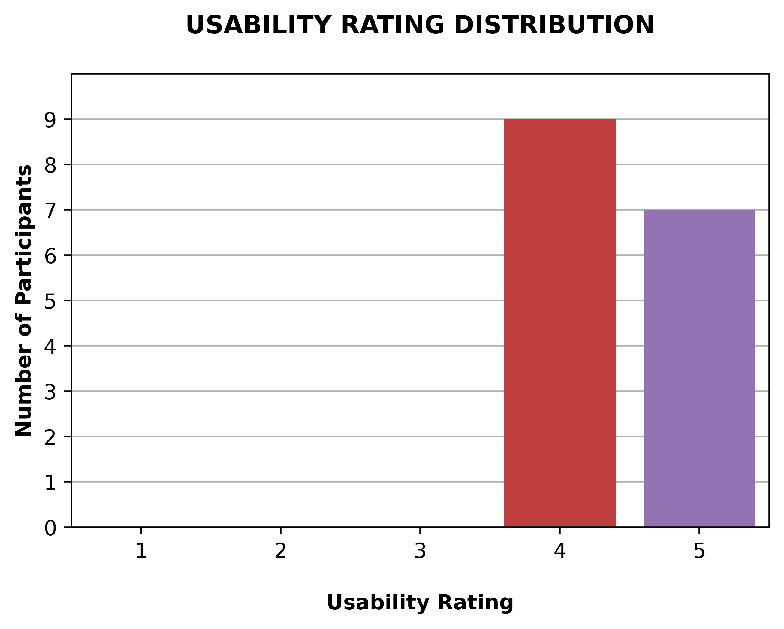
\includegraphics[width=0.7\textwidth]{figures/rating_distribution.pdf}
    \caption{Bar graph showing the distribution of participant ratings regarding the intuitiveness of the interface.}
    \label{fig:rating_distribution}
\end{figure}

\subsubsection{Issues and Improvements}
The next two questions intended to uncover any issues and ways to improve the existing system. Untrained users are more susceptible to encountering bugs because they must engage with the system more extensively to learn how to use it. 7 out of the 16 participants were able to complete their tasks without any problems, however, the remaining experienced one of four distinct issues. The most common issue experienced was a failure after the user interacted with the application during the execution of a background process. This was commonly found to occur during time-intensive routines such as the audio processing after a source is submitted, and the initial retrieval of images. This was a problem that was foreseen during the design phase and intended to be circumvented by displaying a separate loading screen. Its purpose would be two-fold, it would block further user interactions with the frontend and exhibit the estimated time of completion. However, due to time constraints, fully implementing this feature was not realistic when there were several higher priority features that required attention. In hindsight, this can be viewed as the biggest limitation to the current implementation which should be fixed in the next iteration.

Three participants highlighted that they experienced occurrences where none of the images retrieved were relevant to the concepts described in the chunk text. They noted that this made it difficult to ascertain how to proceed, as one had to decide between selecting no images or selecting at least one that exhibits some notion of the concept. From observation, this most frequently occurred when the textual cue itself was ambiguous and described abstract ideas that are difficult to illustrate. For instance, text prompts such as \emph{"Let it go"}, or non-lexical expressions like \emph{"oh oh/la-la"}, which are so common in song lyrics, are particularly difficult to delineate. It is worth noting that the ImageNet-1k dataset, despite its considerable size of more than 1.1 million images, is limited to only one thousand \emph{"synsets"}, as its name implies. Therefore, the system is unable to portray niche ideas solely because it lacks an adequate number of images to represents them. This suggests that a more extensive image dataset could improve retrieval results, not to mention, utilising a larger pre-trained CLIP model.

Some minor issues mentioned in the survey included the uncertainty about which URL of a YouTube video to input. One participant was observed to attain the URL by \emph{"right-clicking on the video"} rather than from the browser address bar. This resulted in a validation error on form submission since the URL pattern (\lstinline|https://youtu.be/...|) was slightly different to the expected pattern (\lstinline|https://www.youtube.com/watch?v=...|). This can be easily resolved either by providing clearer instructions regarding the type of URL required or by modifying the validation check to accommodate both types of URLs. Another participant was unable to navigate back to the Audio page once within a specific Chunk. This could be attributed to the fact that the Audio link is concealed behind the \emph{'Author - Title'} banner, which is only perceived as such on hover. Adding a more explicit 'Back' button to the page can fix this confusion. Lastly, in one of the surveys, a participant expressed doubt about whether to annotate images that effectively conveyed the semantics of the text prompt but were slightly blurred in appearance. This underscores the subjective nature of relevance assessment tasks in general, as ultimately, it is the end viewer's perception that matters which can not be precisely defined. A graded relevance assessment or the removal of blurry images from the dataset could help alleviate this ambiguity, however, more studies must be done to find the best solution.

\subsubsection{Future Feature Ideas}
The final part of the survey asked the participants for suggestions for future features that they would like to see. This provided the opportunity for the application's target users to suggest new feature ideas that would ease relevance annotation effort. There were many good ideas discussed such as adding a sound bite on Chunk pages so that the assessor could listen to the chunk in addition to reading. Identifying the mood from the audio sample could aid in judging abstract text prompts. A different participant proposed the inclusion of a \emph{"Share"} feature that would enable users to directly share the produced video on various social media platforms like YouTube, Facebook, and TikTok. On the topic of integrating the application with other platforms, one respondent recommended enabling the search for YouTube video sources within the site to eliminate the need for the user to manually fetch the right URL.

One participant was assigned the job of creating the ground-truth for the German song, \emph{"99 Luftballons"} by \emph{Nena}, in order to test the effectiveness of the multilingual CLIP model. However, the fact that the participant was not fluent in German made the relevance assessment exceptionally difficult since they needed to translate each chunk phrase into English to understand and identify the relevant images. They went on to suggest incorporating a language translation API that would simplify the assessment process for annotators assessing audio sources that are not in their native language.

Other notable ideas included adding an option to expand the retrieval pool for obscure chunk phrases, adding an option to generate videos from text files, and adding a link to navigate directly to the last edited chunk page. These are discussed in more detail in the Future Work reflection in \ref{sec:future_work}.


\section{Requirement Satisfaction Analysis}
Now that the idiosyncratic requirements have been fully evaluated, the next step is to examine each requirement listed in Chapter \ref{chap:requirements} to form a conclusive assessment of how effectively the project has accomplished its goals.

\subsection{Functional Requirements}
\begin{enumerate}
    \item {\color{forestgreen} $\checkmark$ \textbf{Must Have:} The ability to upload an audio file as an input audio source.}
    \item {\color{forestgreen} $\checkmark$ \textbf{Must Have:} The ability to specify a YouTube video URL as an audio source.}
    \item {\color{forestgreen} $\checkmark$ \textbf{Must Have:} The ability to view the full audio transcription.}
    \item {\color{forestgreen} $\checkmark$ \textbf{Must Have:} The ability to generate an illustrated video for any audio source.}
    \item {\color{forestgreen} $\checkmark$ \textbf{Must Have:} The ability to view the top-$k$ retrieved images for a given audio chunk.}
    \item {\color{forestgreen} $\checkmark$ \textbf{Must Have:} The ability to annotate the most-fitting images for a given audio chunk.}
    \item {\color{forestgreen} $\checkmark$ \textbf{Must Have:} The ability to view the text present in a given audio chunk.}
    \item {\color{forestgreen} $\checkmark$ \textbf{Must Have:} The ability to view the constructed ground-truth data.}
    \item {\color{forestgreen} $\checkmark$ \textbf{Must Have:} The ability to download the constructed ground-truth data in a portable format.}
    \item {\color{forestgreen} $\checkmark$ \textbf{Should Have:} The ability to view previously processed audio sources, generated videos, and constructed ground-truth.}
    \item {\color{forestgreen} $\checkmark$ \textbf{Should Have:} The ability to edit previously made ground-truths.}
    \item {\color{forestgreen} $\checkmark$ \textbf{Should Have:} The ability to upload audio sources of any language.}
    \item \label{reqs:13} {\color{brickred} $\times$ \textbf{Could Have:} The ability to load ground-truths for editing.}
    \item \label{reqs:14} {\color{golden} $\sim$ \textbf{Could Have:} The ability to reconfigure the static image collection location.}
    \item \label{reqs:15} {\color{brickred} $\times$ \textbf{*Could Have:} The ability to view the percentage complete for ground-truth construction of processed audio sources.}
    \item {\color{forestgreen} $\checkmark$ \textbf{*Could Have:} The ability to save or skip chunks with repeating textual content when ground-truth constructing.}
    \item {\color{forestgreen} $\checkmark$ \textbf{*Could Have:} The ability to view the timestamp information of audio chunks.}
\end{enumerate}

\subsection{Non-Functional Requirements}
\begin{enumerate}[resume]
    \item {\color{forestgreen} $\checkmark$ \textbf{Must Have:} The system using a static collection of images for repeatably consistent ground-truth construction.}
    \item {\color{forestgreen} $\checkmark$ \textbf{Should Have:} The application being accessible from any Operating System platform.}
    \item {\color{forestgreen} $\checkmark$ \textbf{Should Have:} The application having a presentable user interface that is easy for any user to understand and learn quickly.}
    \item {\color{forestgreen} $\checkmark$ \textbf{Should Have:} The application with appropriate error handling.}
    \item {\color{forestgreen} $\checkmark$ \textbf{Should Have:} The application being fast and responsive.}
    \item {\color{forestgreen} $\checkmark$ \textbf{Should Have:} The system being able to recognise music tracks to automatically retrieve the artist name and song title.}
    \item {\color{forestgreen} $\checkmark$ \textbf{Should Have:} The application being able to transcribe any audio source providing phrase-level timestamps.}
    \item {\color{forestgreen} $\checkmark$ \textbf{Should Have:} The system retrieving more relevant images by leveraging semantics of natural language as well as visual features.}
    \item {\color{forestgreen} $\checkmark$ \textbf{Should Have:} The videos being generated in a more reasonable amount of time than the prior system.}
    \item {\color{forestgreen} $\checkmark$ \textbf{Should Have:} The generated video having a higher resolution than the prior system.}
    \item \label{reqs:28} {\color{brickred} $\times$  \textbf{Should Have:} The application displaying progress bars for long loading times.}
    \item {\color{forestgreen} $\checkmark$ \textbf{Could Have:} The application being designed with extensibility in mind so that the image collection can be reconfigured.}
    \item {\color{forestgreen} $\checkmark$ \textbf{Could Have:} The videos including text as well as images.}
    \item {\color{forestgreen} $\checkmark$ \textbf{Could Have:} The application visually differentiating between previously processed audio sources.}
    \item \label{reqs:32} {\color{brickred} $\times$  \textbf{Could Have:} The system performing tempo or beat analysis to appropriately time image changes.}
\end{enumerate}

The project was able to satisfy the majority of the requirement specification, with over 85\% (27/32) of the requirements being fulfilled. More importantly, all of the highest priority \textbf{Must Haves} were satisfied. The status of requirement \textbf{\#\ref{reqs:14}} is amber because the feature has not been incorporated into the application's frontend. Nevertheless, the image collection can be substituted in the source code owing to the program's extendable design. Overall, it can be safely asserted that the project has achieved its aim, with the final product functioning largely in accordance with its original intent.


\section{Summary}
This chapter provided an extensive evaluation of the final product in order to check if it fulfilled the fundamental goals of the project. This was done by analysing the original system requirements specified within Chapter \ref{chap:requirements}. In order to evaluate the more abstract requirements, several experiments were conducted to gather empirical evidence of its effectiveness. Overall, it is safe to conclude that the project delivered a functional product that met most of the primary objectives. 

% How good is your solution? How well did you solve the general problem, and what evidence do you have to support that?

% \section{Guidance}
% \begin{itemize}
%     \item
%         Ask specific questions that address the general problem.
%     \item
%         Answer them with precise evidence (graphs, numbers, statistical
%         analysis, qualitative analysis).
%     \item
%         Be fair and be scientific.
%     \item
%         The key thing is to show that you know how to evaluate your work, not
%         that your work is the most amazing product ever.
% \end{itemize}

% \section{Evidence}
% Make sure you present your evidence well. Use appropriate visualisations, 
% reporting techniques and statistical analysis, as appropriate. The point is not
% to dump all the data you have but to present an argument well supported by evidence gathered.

% If you use numerical evidence, specify reasonable numbers of significant digits; don't state ``18.41141\% of users were successful'' if you only had 20 users. If you average \textit{anything}, present both a measure of central tendency (e.g. mean, median) \textit{and} a measure of spread (e.g. standard deviation, min/max, interquartile range).

% You can use \texttt{siunitx} to define units, space numbers neatly, and set the precision for the whole LaTeX document. 

% % setup siunitx to have two decimal places
% \sisetup{
% 	round-mode = places,
% 	round-precision = 2
% }

% For example, these numbers will appear with two decimal places: \num{3.141592}, \num{2.71828}, and this one will appear with reasonable spacing \num{1000000}.



% If you use statistical procedures, make sure you understand the process you are using,
% and that you check the required assumptions hold in your case. 

% If you visualise, follow the basic rules, as illustrated in Figure \ref{fig:boxplot}:
% \begin{itemize}
% \item Label everything correctly (axis, title, units).
% \item Caption thoroughly.
% \item Reference in text.
% \item \textbf{Include appropriate display of uncertainty (e.g. error bars, Box plot)}
% \item Minimize clutter.
% \end{itemize}

% See the file \texttt{guide\_to\_visualising.pdf} for further information and guidance.

% \begin{figure}[htb]
%     \centering
%     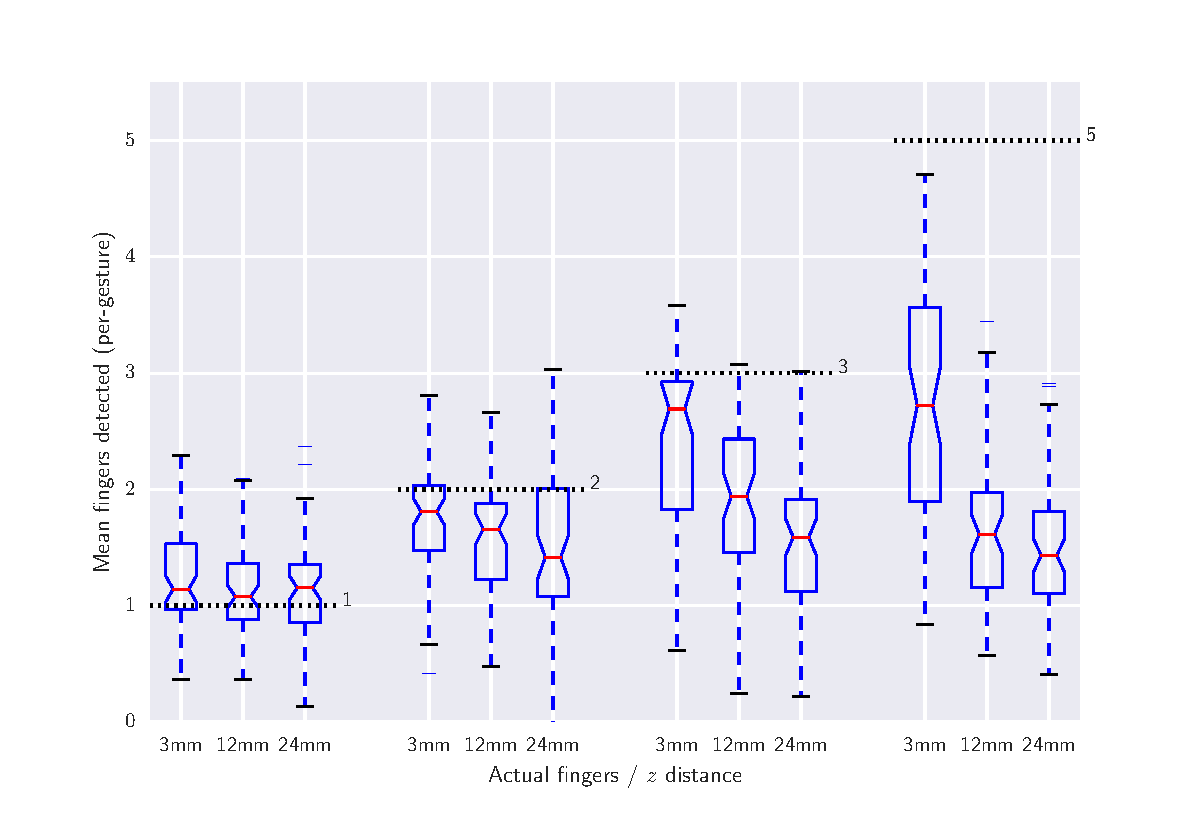
\includegraphics[width=1.0\linewidth]{figures/boxplot_finger_distance.pdf}    

%     \caption{Average number of fingers detected by the touch sensor at different heights above the surface, averaged over all gestures. Dashed lines indicate
%     the true number of fingers present. The Box plots include bootstrapped uncertainty notches for the median. It is clear that the device is biased toward 
%     undercounting fingers, particularly at higher $z$ distances.
%     }

%     % use the notation fig:name to cross reference a figure
%     \label{fig:boxplot} 
% \end{figure}


%==================================================================================================
\chapter{Conclusion}    
\section{Summary}
This project aimed to create two new technologies, namely a new Automated Videography system that improves on the previous product built by \cite{parker} and a ground-truth annotation interface. In the end, the project resulted in a successful system that can generate a video composed of relevant imagery to accompany any audio source. Furthermore, a user-friendly interface was devised, that aims to simplify the process of assessing the relevance of images derived from textual queries. This interface effectively streamlines this task of ground-truth construction intended for the quantitative evaluation of automatic videography systems. To the best of our knowledge, this is something that is missing from existing annotation software.

% Background research into the history of relevance assessment within the field of Information Retrieval was conducted, as well as exploring intelligent solutions to the limitations of the preceding videography system. The advent of new image-text multimodal embedding models offered new approaches to the problem that could incorporate the natural language semantices to retrieve more relevant imagery enhancing content creation.

The project followed an agile software development framework by constructing user scenarios in order to facilitate clear system requirements and design. The application was implemented with extensibility in mind in order to ease the addition of new features. The system and its accompanying frontend interface were subsequently evaluated in order to determine whether all the pre-conceived goals have been fulfilled. This involved running three main experiments. 

Firstly, the implementations of more efficient image indexing and retrieving methods were explored using FAISS which were unsuccessful. This did not cause a huge hindrance to the project since the system's exhaustive search was found to be sufficiently fast with the ImageNet-1k collection. Secondly, a comparison of the generation times of the new and preceding videography systems was done. The new system resulted in a mean video generation time of 4 minutes and 29 seconds, reducing waiting times by 42\%. The final experiment entailed testing the usability of the ground-truth annotation interface with sixteen participants. On average, the respondents rated the intuitiveness of the interface 4.4 out of 5. In addition, every participant was able to complete their ground-truth construction task. This data is made available in the project GitHub repository\footnote{\url{https://tinyurl.com/2p8he6sr}}. The purpose of this data is to enable reliable and repeatable performance evaluations of automatic videography systems while also alleviating the need for subjective user evaluations.


\section{Reflection}
Looking back, many valuable insights were gained throughout the development process of the project. It underlined the importance of careful organisation in order to manage such a large-scale individual project. Breaking down substantial tasks into smaller, practicable workloads, that could be tackled iteratively, proved vital to the successful completion of the project within the specified timeframe. In addition, it was learned early on that planning out the next steps within the project lifecycle was especially important. This softened the impact of major obstacles that would have necessitated retracing and re-evaluation of the problem. One of the biggest flaws made during the project was the mis-prioritisation of the \textbf{Should Have} requirement \textbf{\#\ref{reqs:28}}. The lack of a loading page became the cause of the leading fault encountered during usability testing. In hindsight, it is apparent that this feature should have been ranked higher as a \textbf{Must Have} in order to enforce its implementation sooner.


\section{Future Work}
\label{sec:future_work}
This project offers many potential future prospects both in terms of fixing issues identified in the final evaluation and the addition of new features. First and foremost, the missed requirement for an intermediary loading page should be put in effect for time-consuming processing tasks. Secondly, this project has a clear motivation to move toward using larger image collections for better relevance assessment and videography results. However, the current implementation employs exhaustive search and retrievals which can not be scaled to datasets spanning hundreds of millions of images. Further work with FAISS should be conducted in order to improve efficiency while also maintaining high retrieval accuracy. Possible routes could be reducing the dimension size of feature vectors from 512 to 128 using Principle Component Analysis (PCA) to identify salient dimensions. Smaller feature vectors could aid the indexing operation providing better clusters.

There were several potential features that were suggested by the participants in the usability survey. To name a few, adding an audio sample to each Chunk page so that assessors can judge relevance better based on both audio and text. Adding an option to directly share generated videos to social media platforms. A possible integration of the YouTube search API for further user-friendliness, bypassing the requirement of inputting a URL. Adding a language translation layer to pages so that it is not required for assessors to be native speakers to be effective in labelling images. In some cases showing the top ten images is not enough to uncover relevance, adding a button to expand the retrieval pool depth could help in this aspect. Instead of only allowing video generation from audio sources, users may want to create a video from a written transcription. Text-to-speech tools can then be used to accompany the final video. As demonstrated, the end product provides ample scope for expansion to further our goal of easing content creation and relevance assessment.

On a final note, the work carried out by \cite{parker} has been approved for inclusion into the 2023 European Conference on Information Retrieval (ECIR) proceedings upon revision of the original demonstration paper. The paper is available for viewing at \cite{videography} and the final product of this project will be subsequently showcased at the conference. Similarly, we intend to submit this project's work to the 2023 Conference on Information and Knowledge Management (CKIM).


% Summarise the whole project for a lazy reader who didn't read the rest (e.g. a prize-awarding committee). This chapter should be short in most dissertations; maybe one to three pages.
% \section{Guidance}
% \begin{itemize}
%     \item
%         Summarise briefly and fairly.
%     \item
%         You should be addressing the general problem you introduced in the
%         Introduction.        
%     \item
%         Include summary of concrete results (``the new compiler ran 2x
%         faster'')
%     \item
%         Indicate what future work could be done, but remember: \textbf{you
%         won't get credit for things you haven't done}.
% \end{itemize}

% \section{Summary}
% Summarise what you did; answer the general questions you asked in the introduction. What did you achieve? Briefly describe what was built and summarise the evaluation results.

% \section{Reflection}
% Discuss what went well and what didn't and how you would do things differently if you did this project again.

% \section{Future work}
% Discuss what you would do if you could take this further -- where would the interesting directions to go next be? (e.g. you got another year to work on it, or you started a company to work on this, or you pursued a PhD on this topic)

%=================================================================================================
%  APPENDICES  

\begin{appendices}
% \chapter{Appendices}
% Use separate appendix chapters for groups of ancillary material that support your dissertation. 
% Typical inclusions in the appendices are:

% \begin{itemize}
% \item
%   Copies of ethics approvals (you must include these if you needed to get them)
% \item
%   Copies of questionnaires etc. used to gather data from subjects. Don't include
%   voluminous data logs; instead submit these electronically alongside your source code.
% \item
%   Extensive tables or figures that are too bulky to fit in the main body of
%   the report, particularly ones that are repetitive and summarised in the body.
% \item Outline of the source code (e.g. directory structure), 
%     or other architecture documentation like class diagrams.
% \item User manuals, and any guides to starting/running the software. 
% Your equivalent of \texttt{readme.md} should be included.
% \end{itemize}

% \textbf{Don't include your source code in the appendices}. It will be
% submitted separately.
\chapter{Walkthrough of Final Application}
\label{app:walkthrough}
\begin{figure}
    \centering
    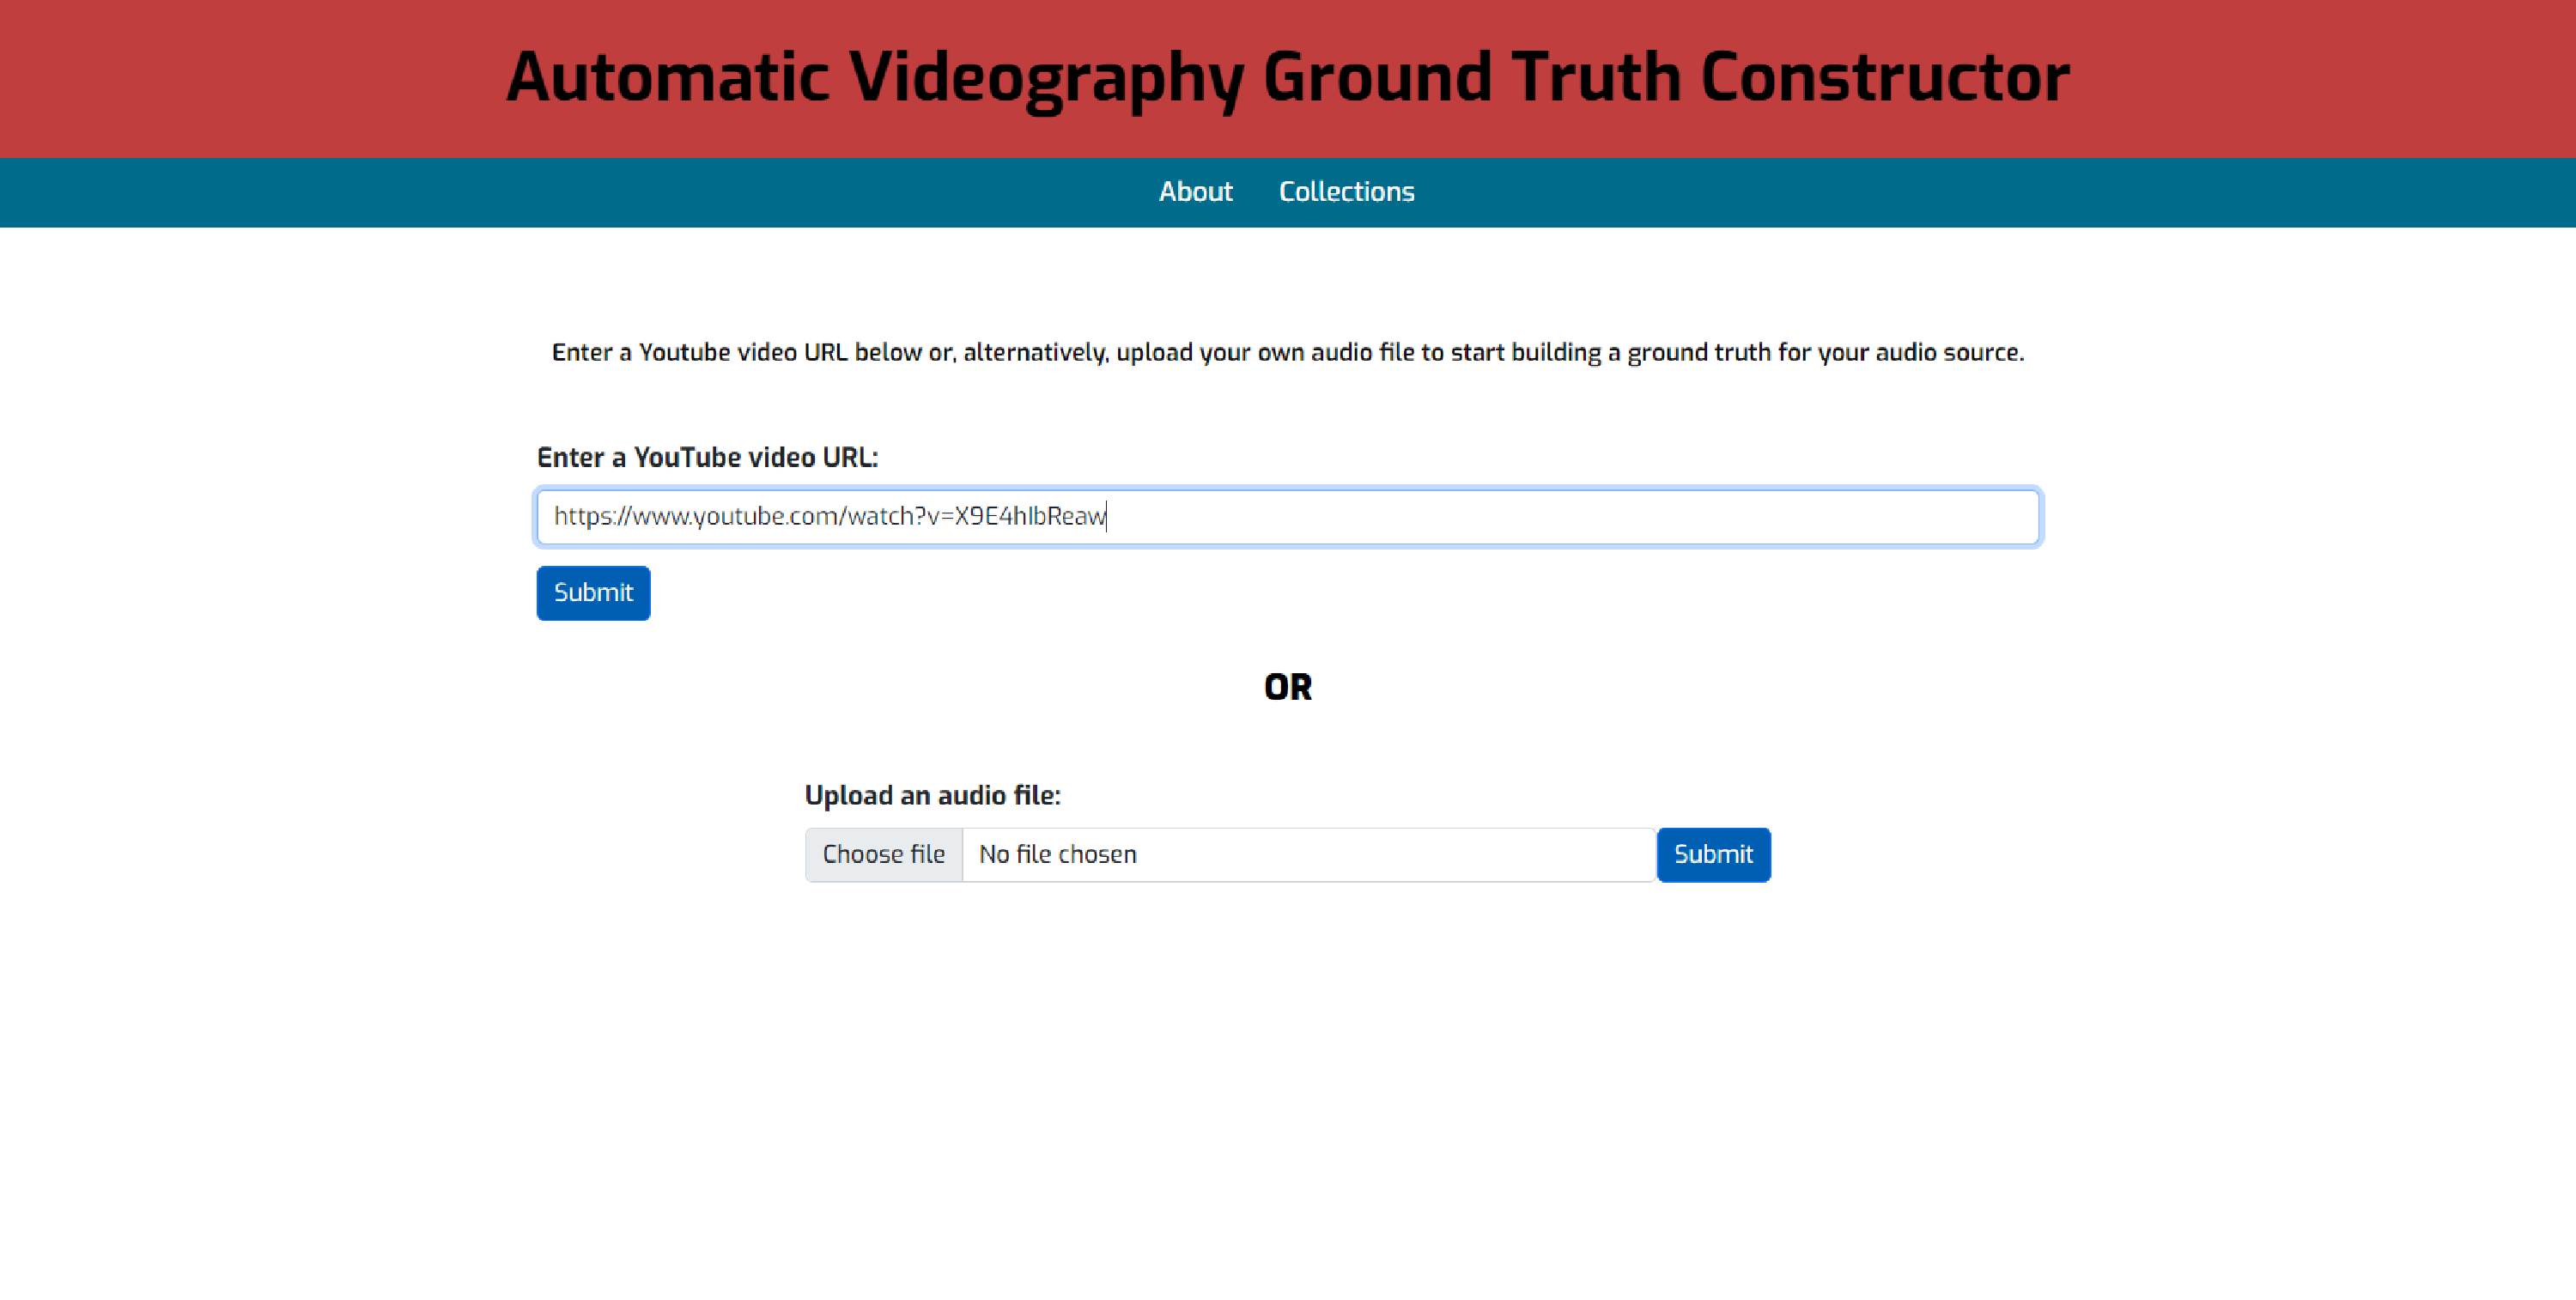
\includegraphics[width=1\textwidth]{figures/walkthrough_home_page.pdf}
    \caption{Example of using the Home page by inputting a YouTube video URL for the song "Jigsaw Falling Into Place" by Radiohead}
    \label{fig:walkthrough_home_page}
\end{figure}

\begin{figure}
    \centering
    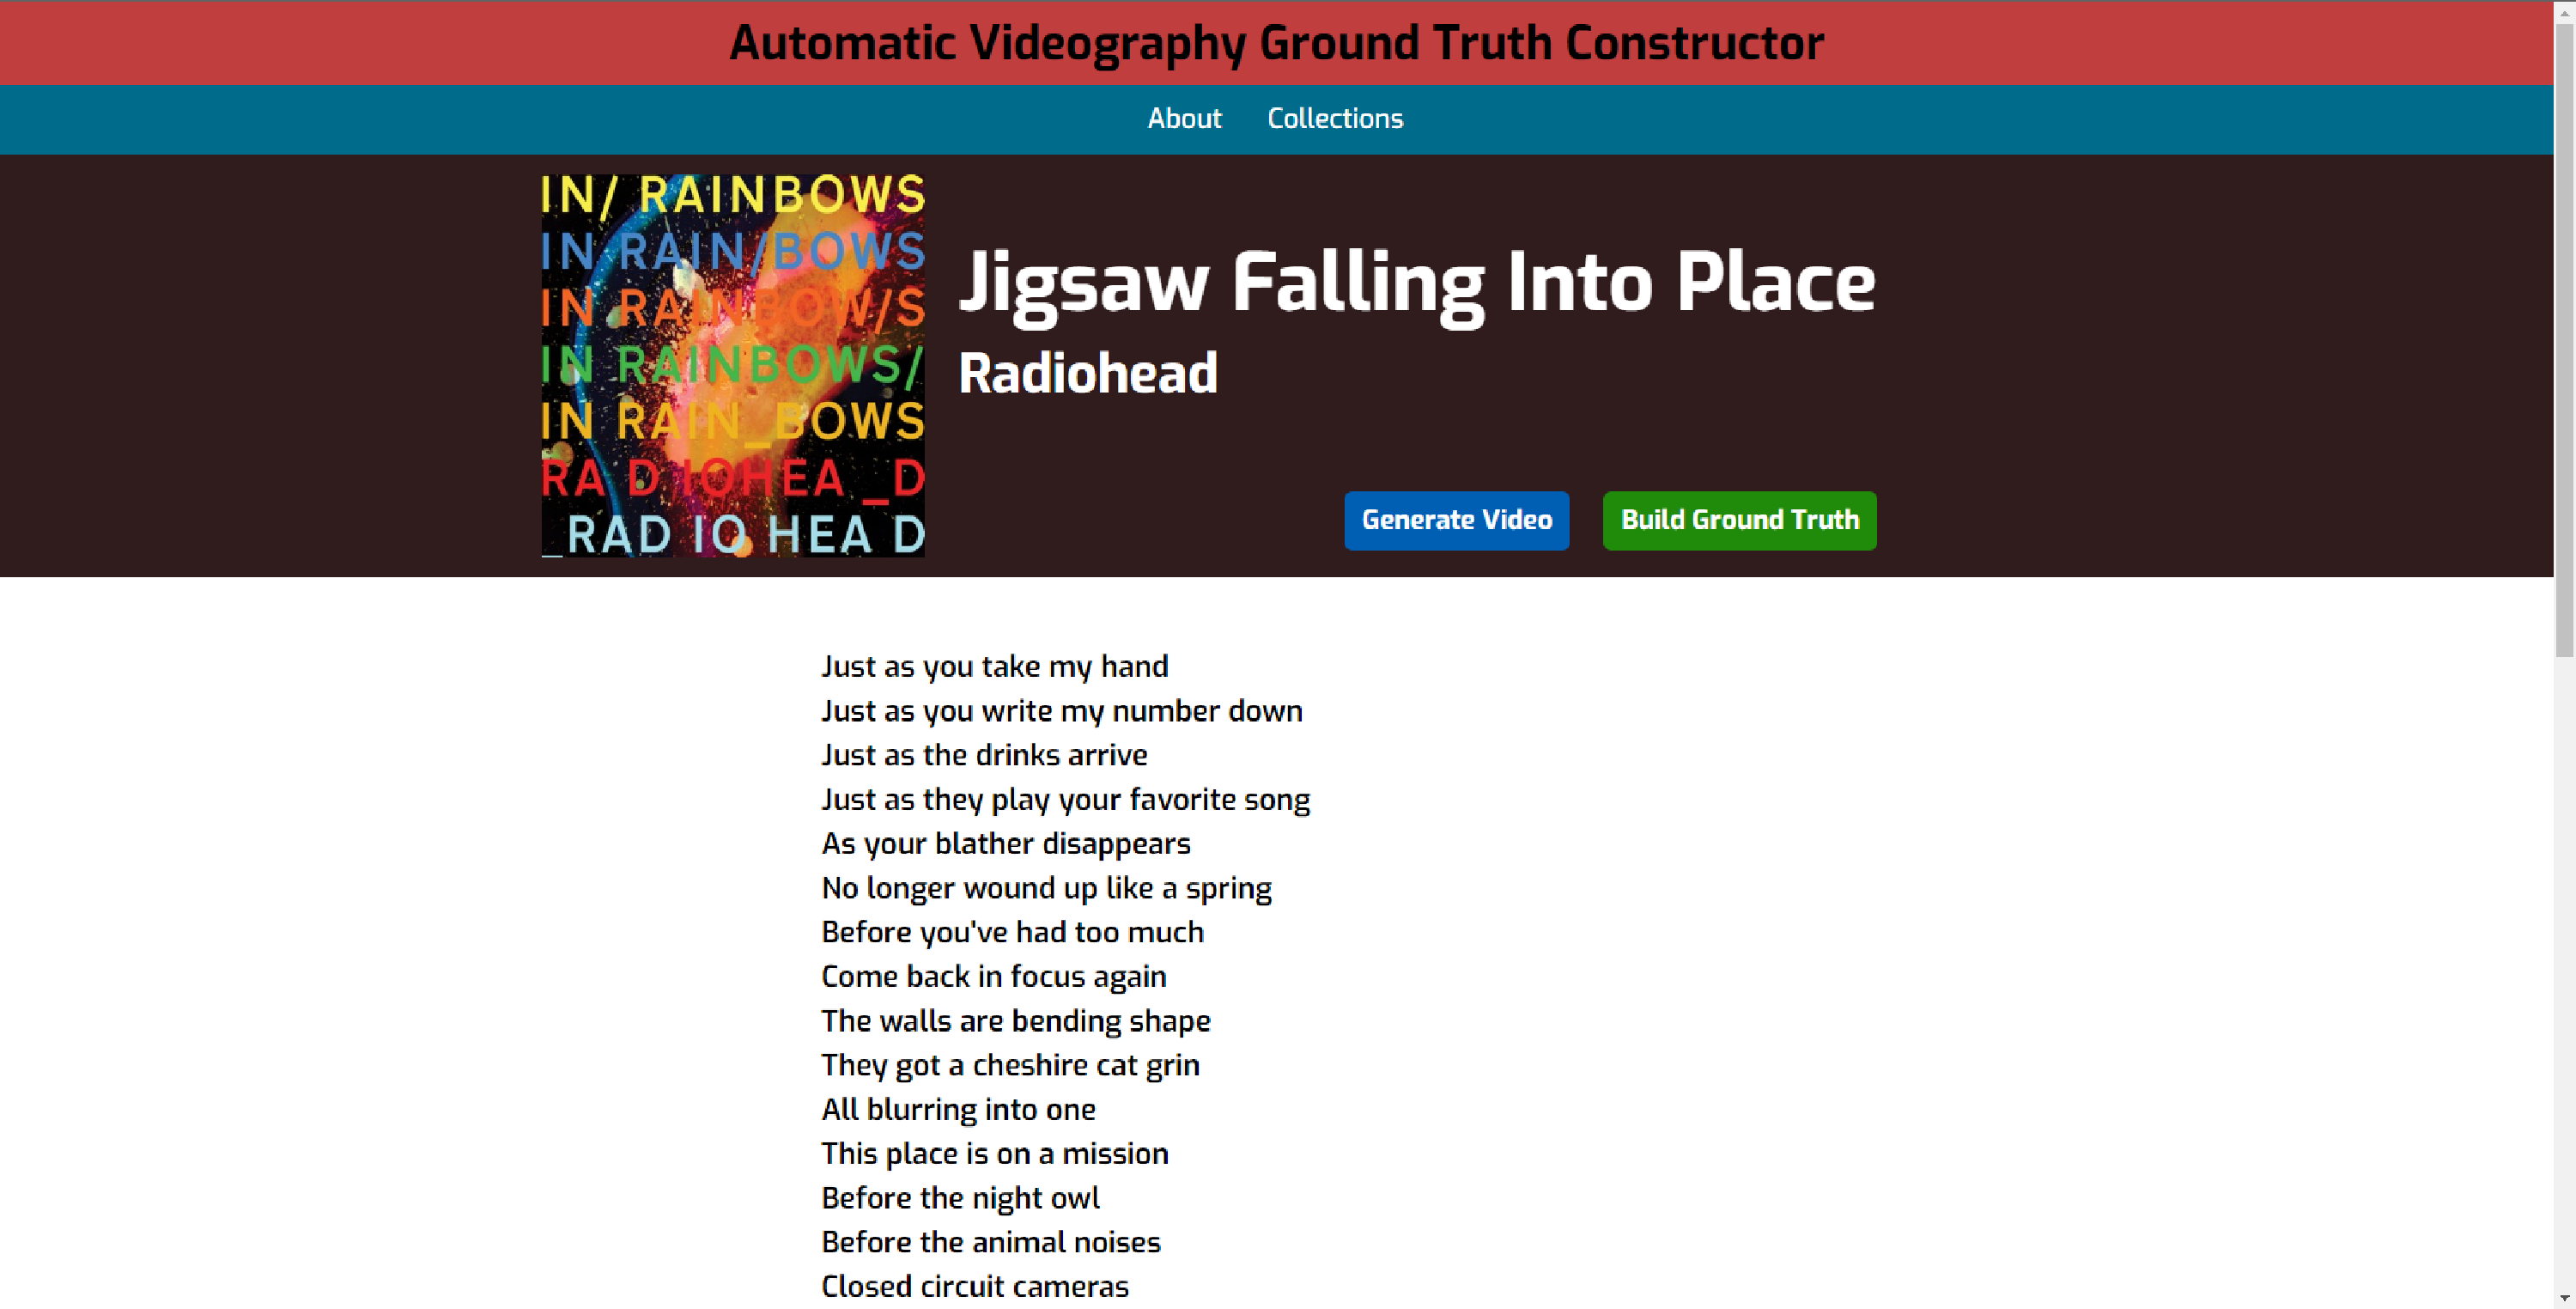
\includegraphics[width=1\textwidth]{figures/walkthrough_audio_page.pdf}
    \caption{Resulting Audio page for the song "Jigsaw Falling Into Place" by Radiohead}
    \label{fig:walkthrough_audio_page}
\end{figure}

\begin{figure}
    \centering
    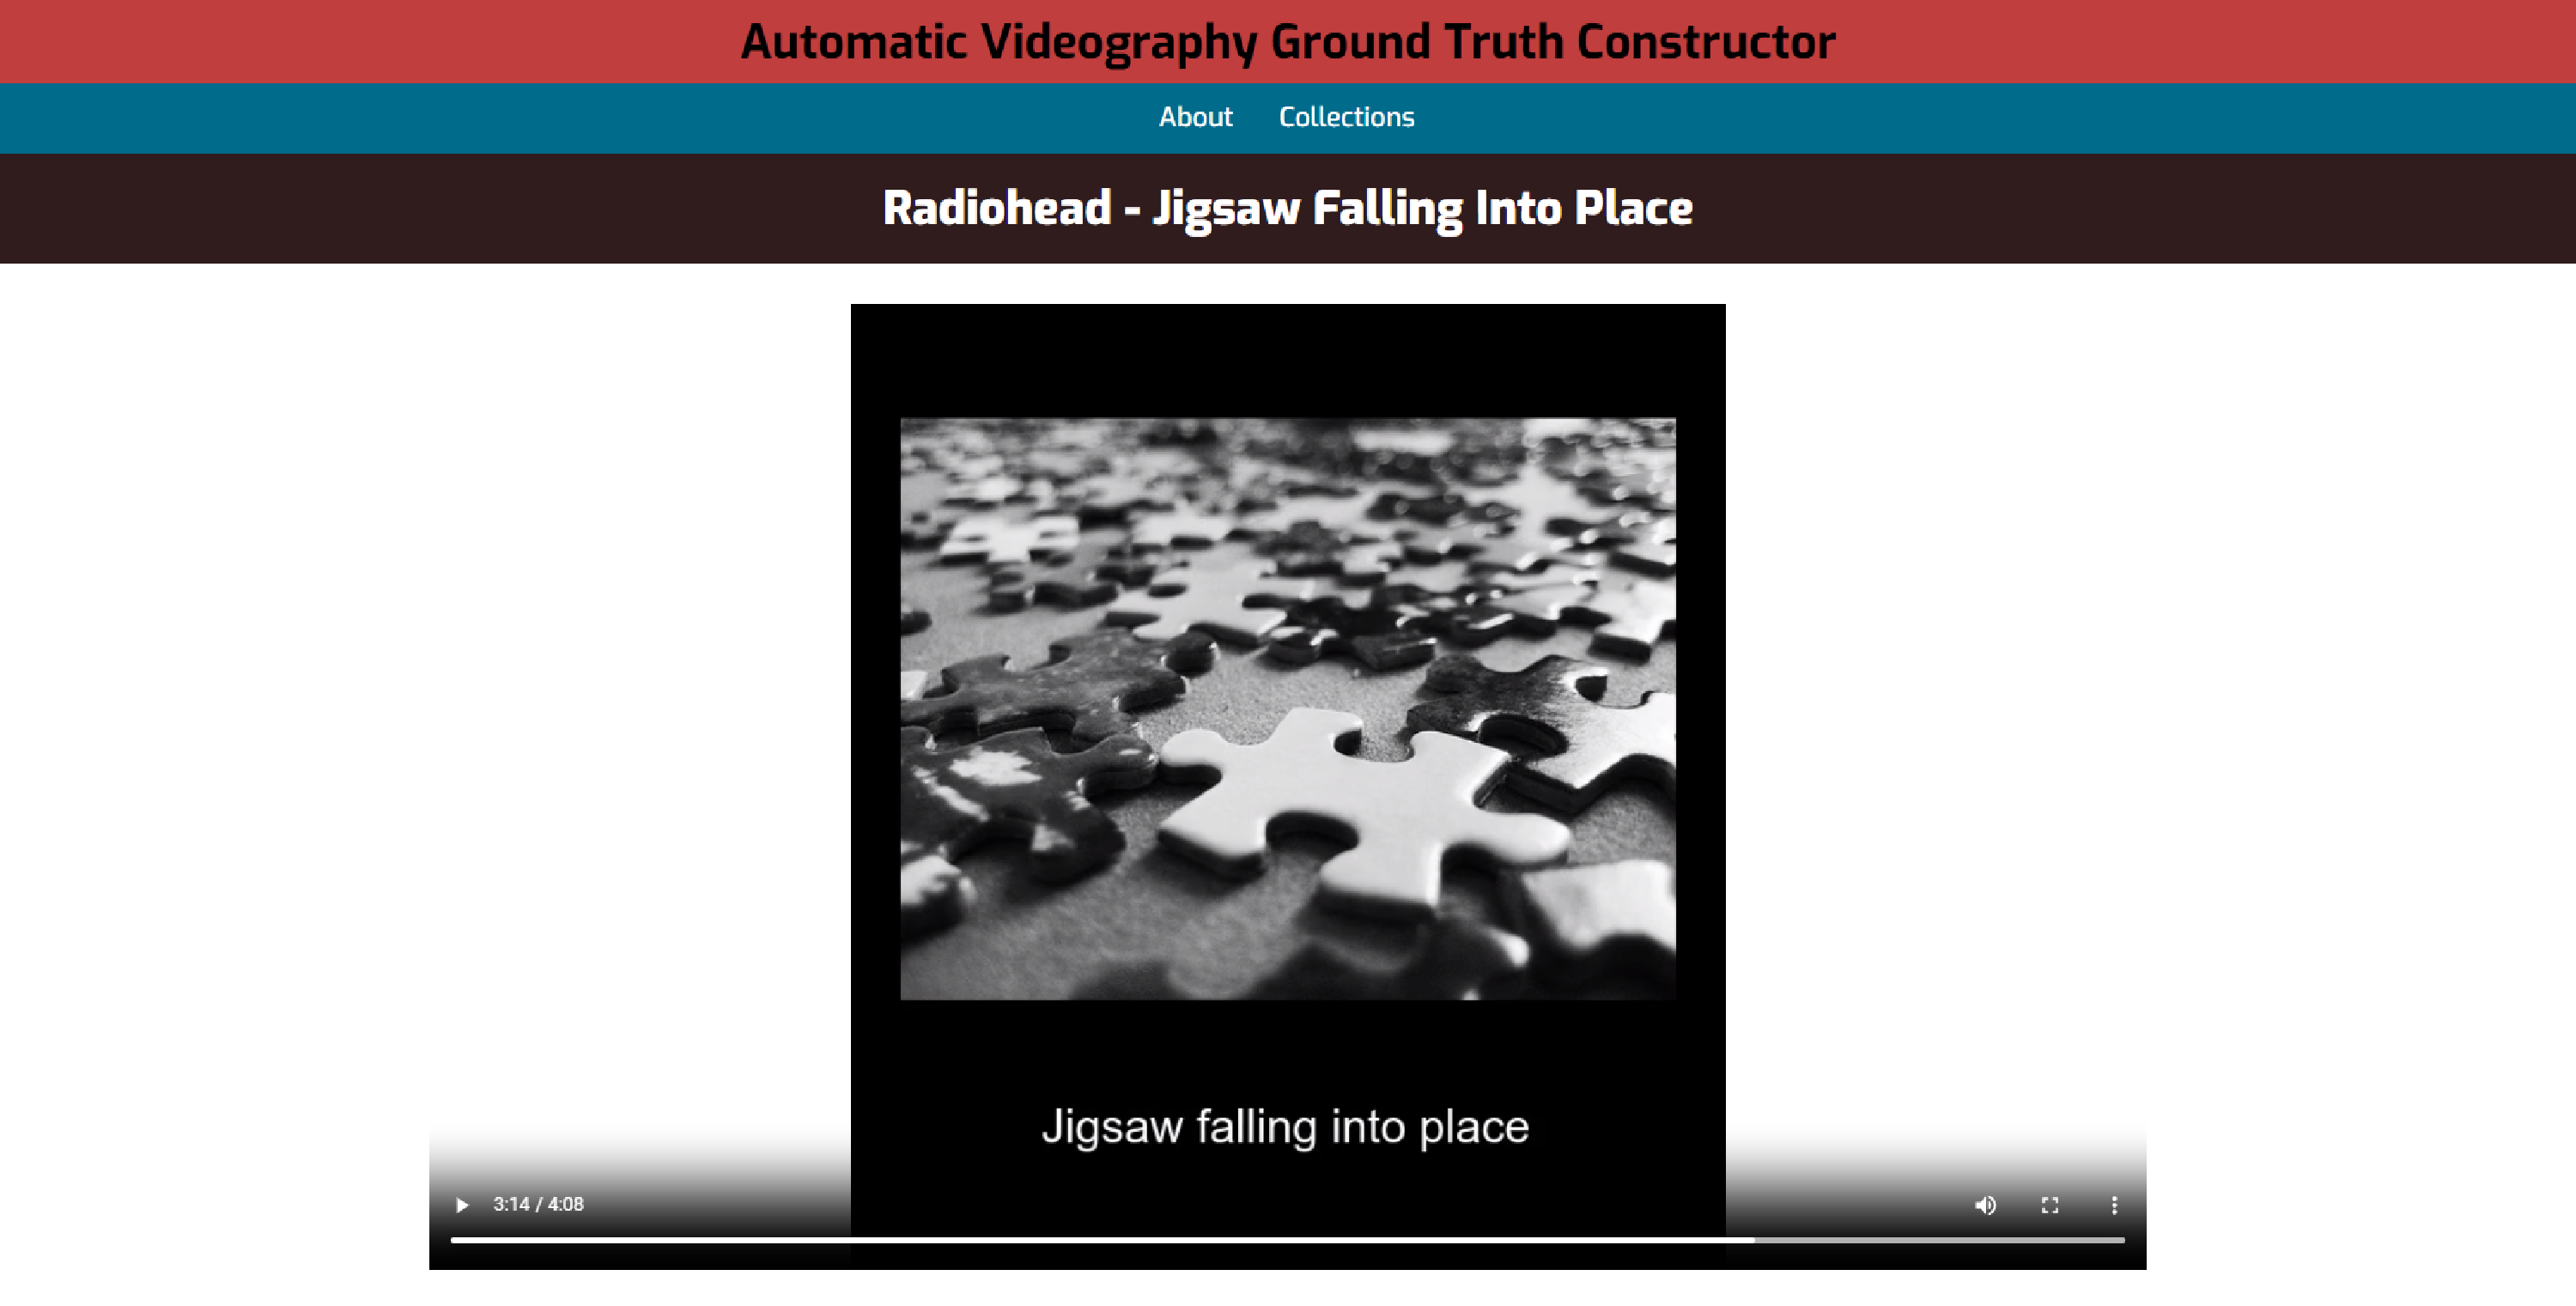
\includegraphics[width=1\textwidth]{figures/walkthrough_video_page.pdf}
    \caption{Resulting Video page for the song "Jigsaw Falling Into Place" by Radiohead}
    \label{fig:walkthrough_video_page}
\end{figure}

\begin{figure}
    \centering
    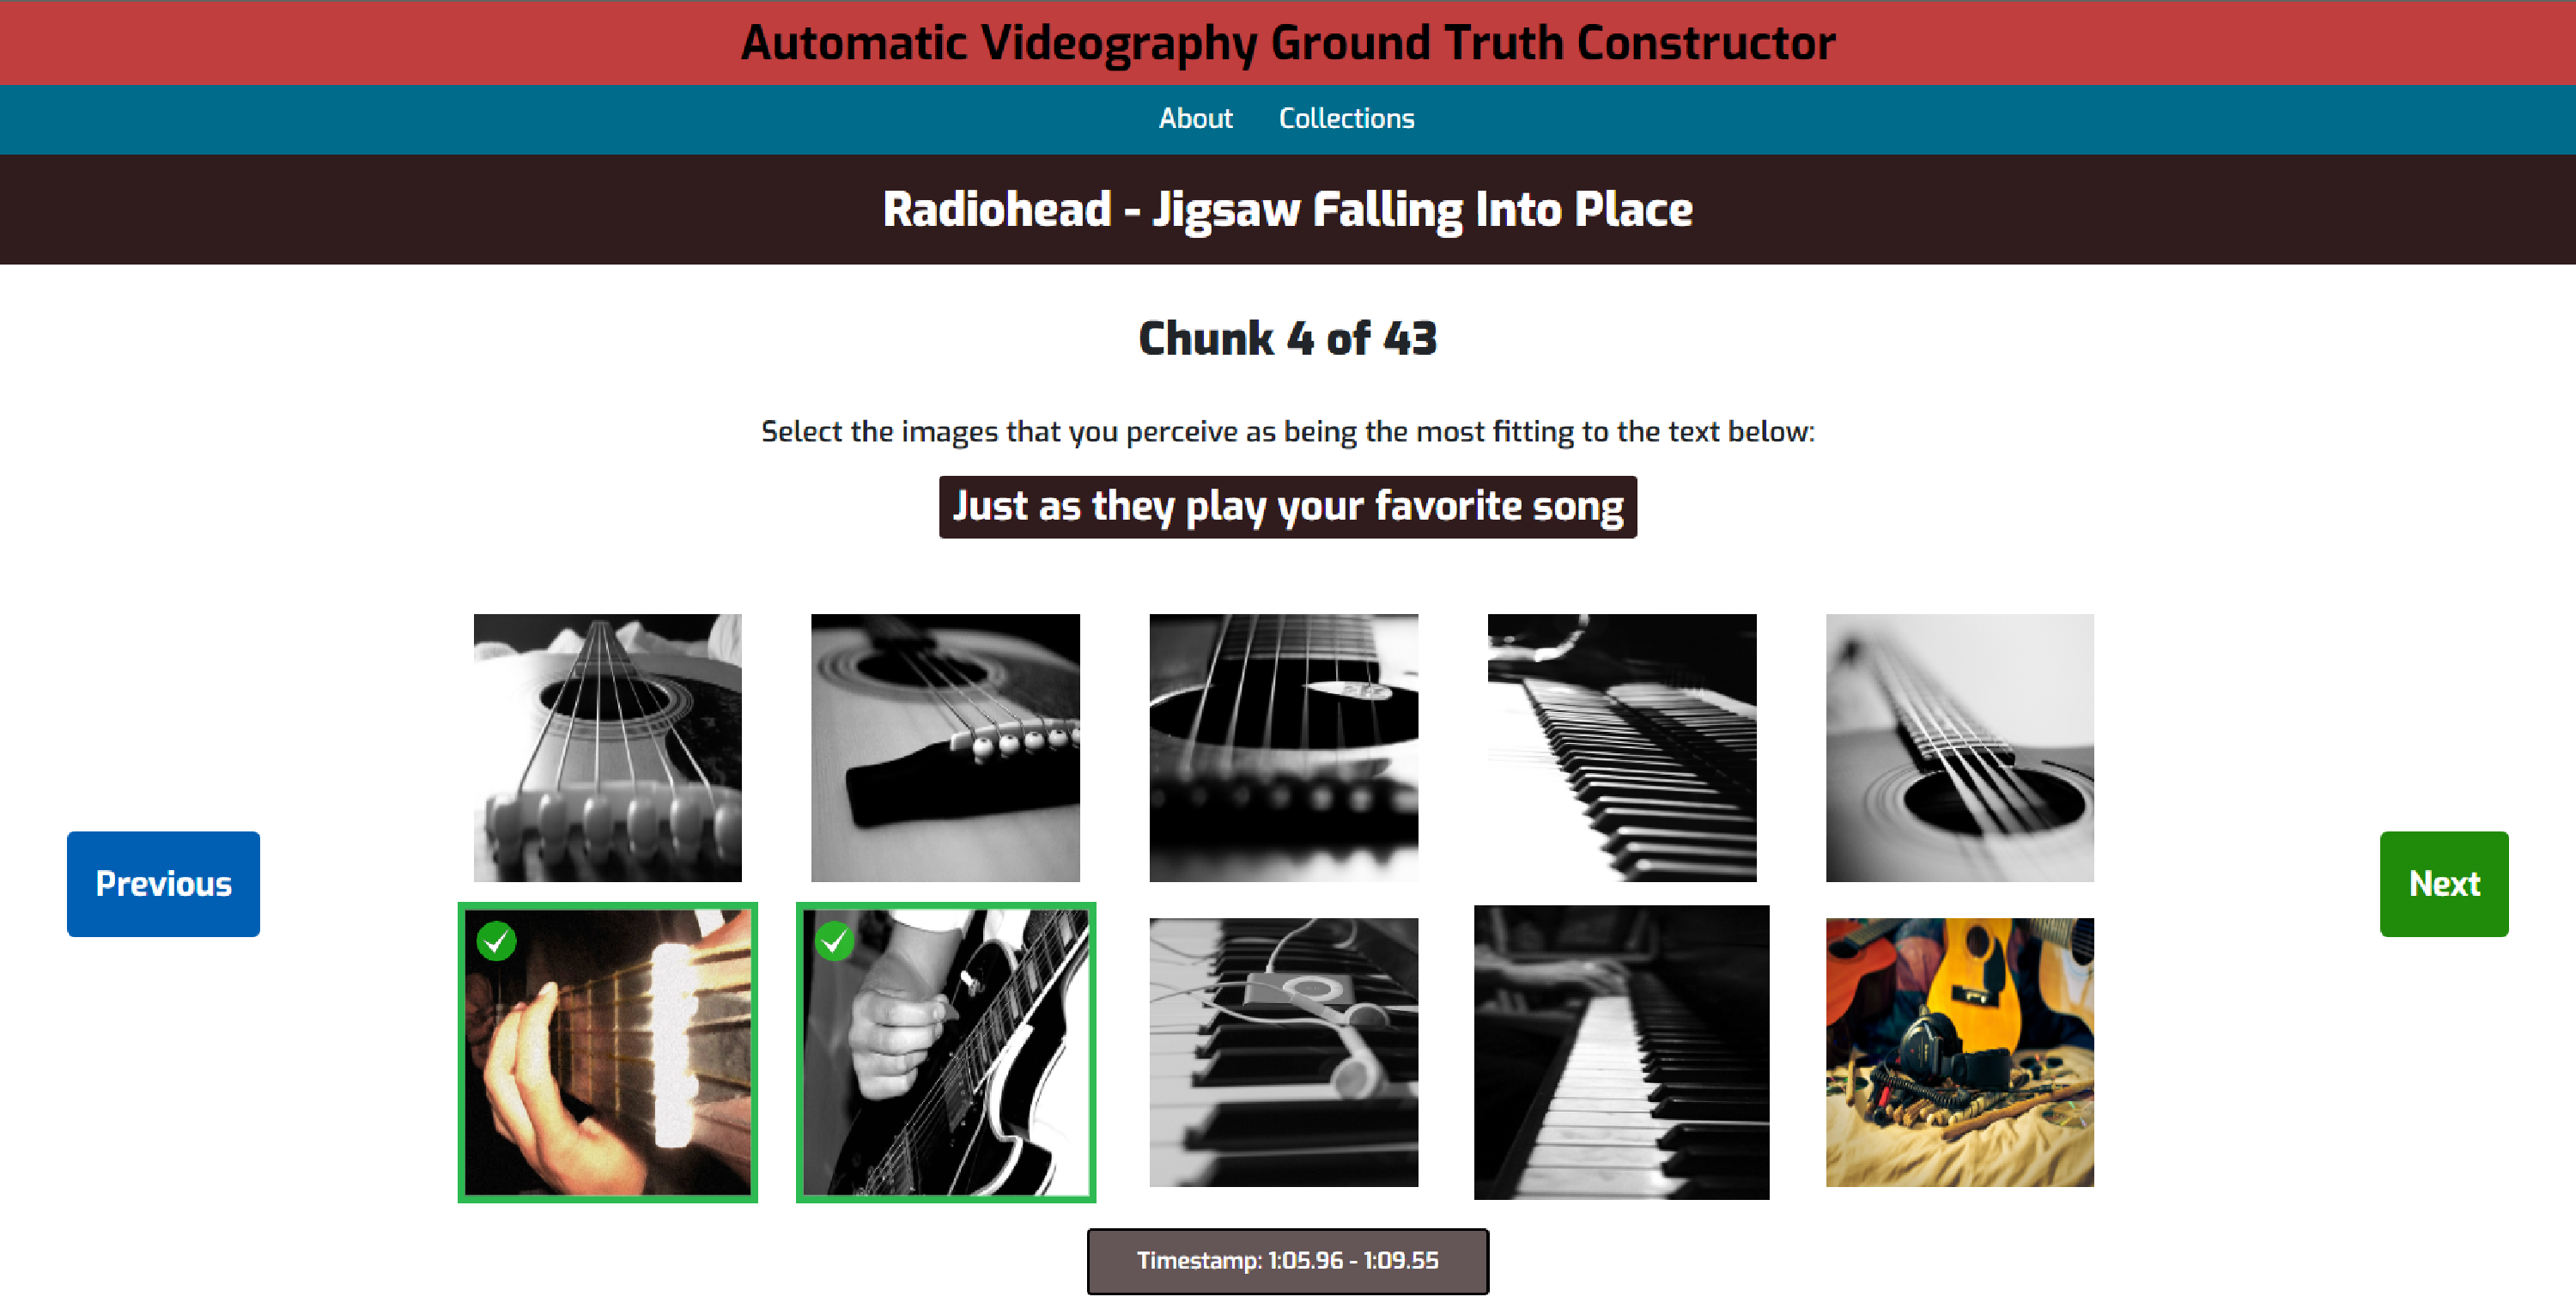
\includegraphics[width=1\textwidth]{figures/walkthrough_chunk_page.pdf}
    \caption{Example of annotating images for Chunk 4 for the song "Jigsaw Falling Into Place" by Radiohead}
    \label{fig:walkthrough_chunk_page}
\end{figure}

\begin{figure}
    \centering
    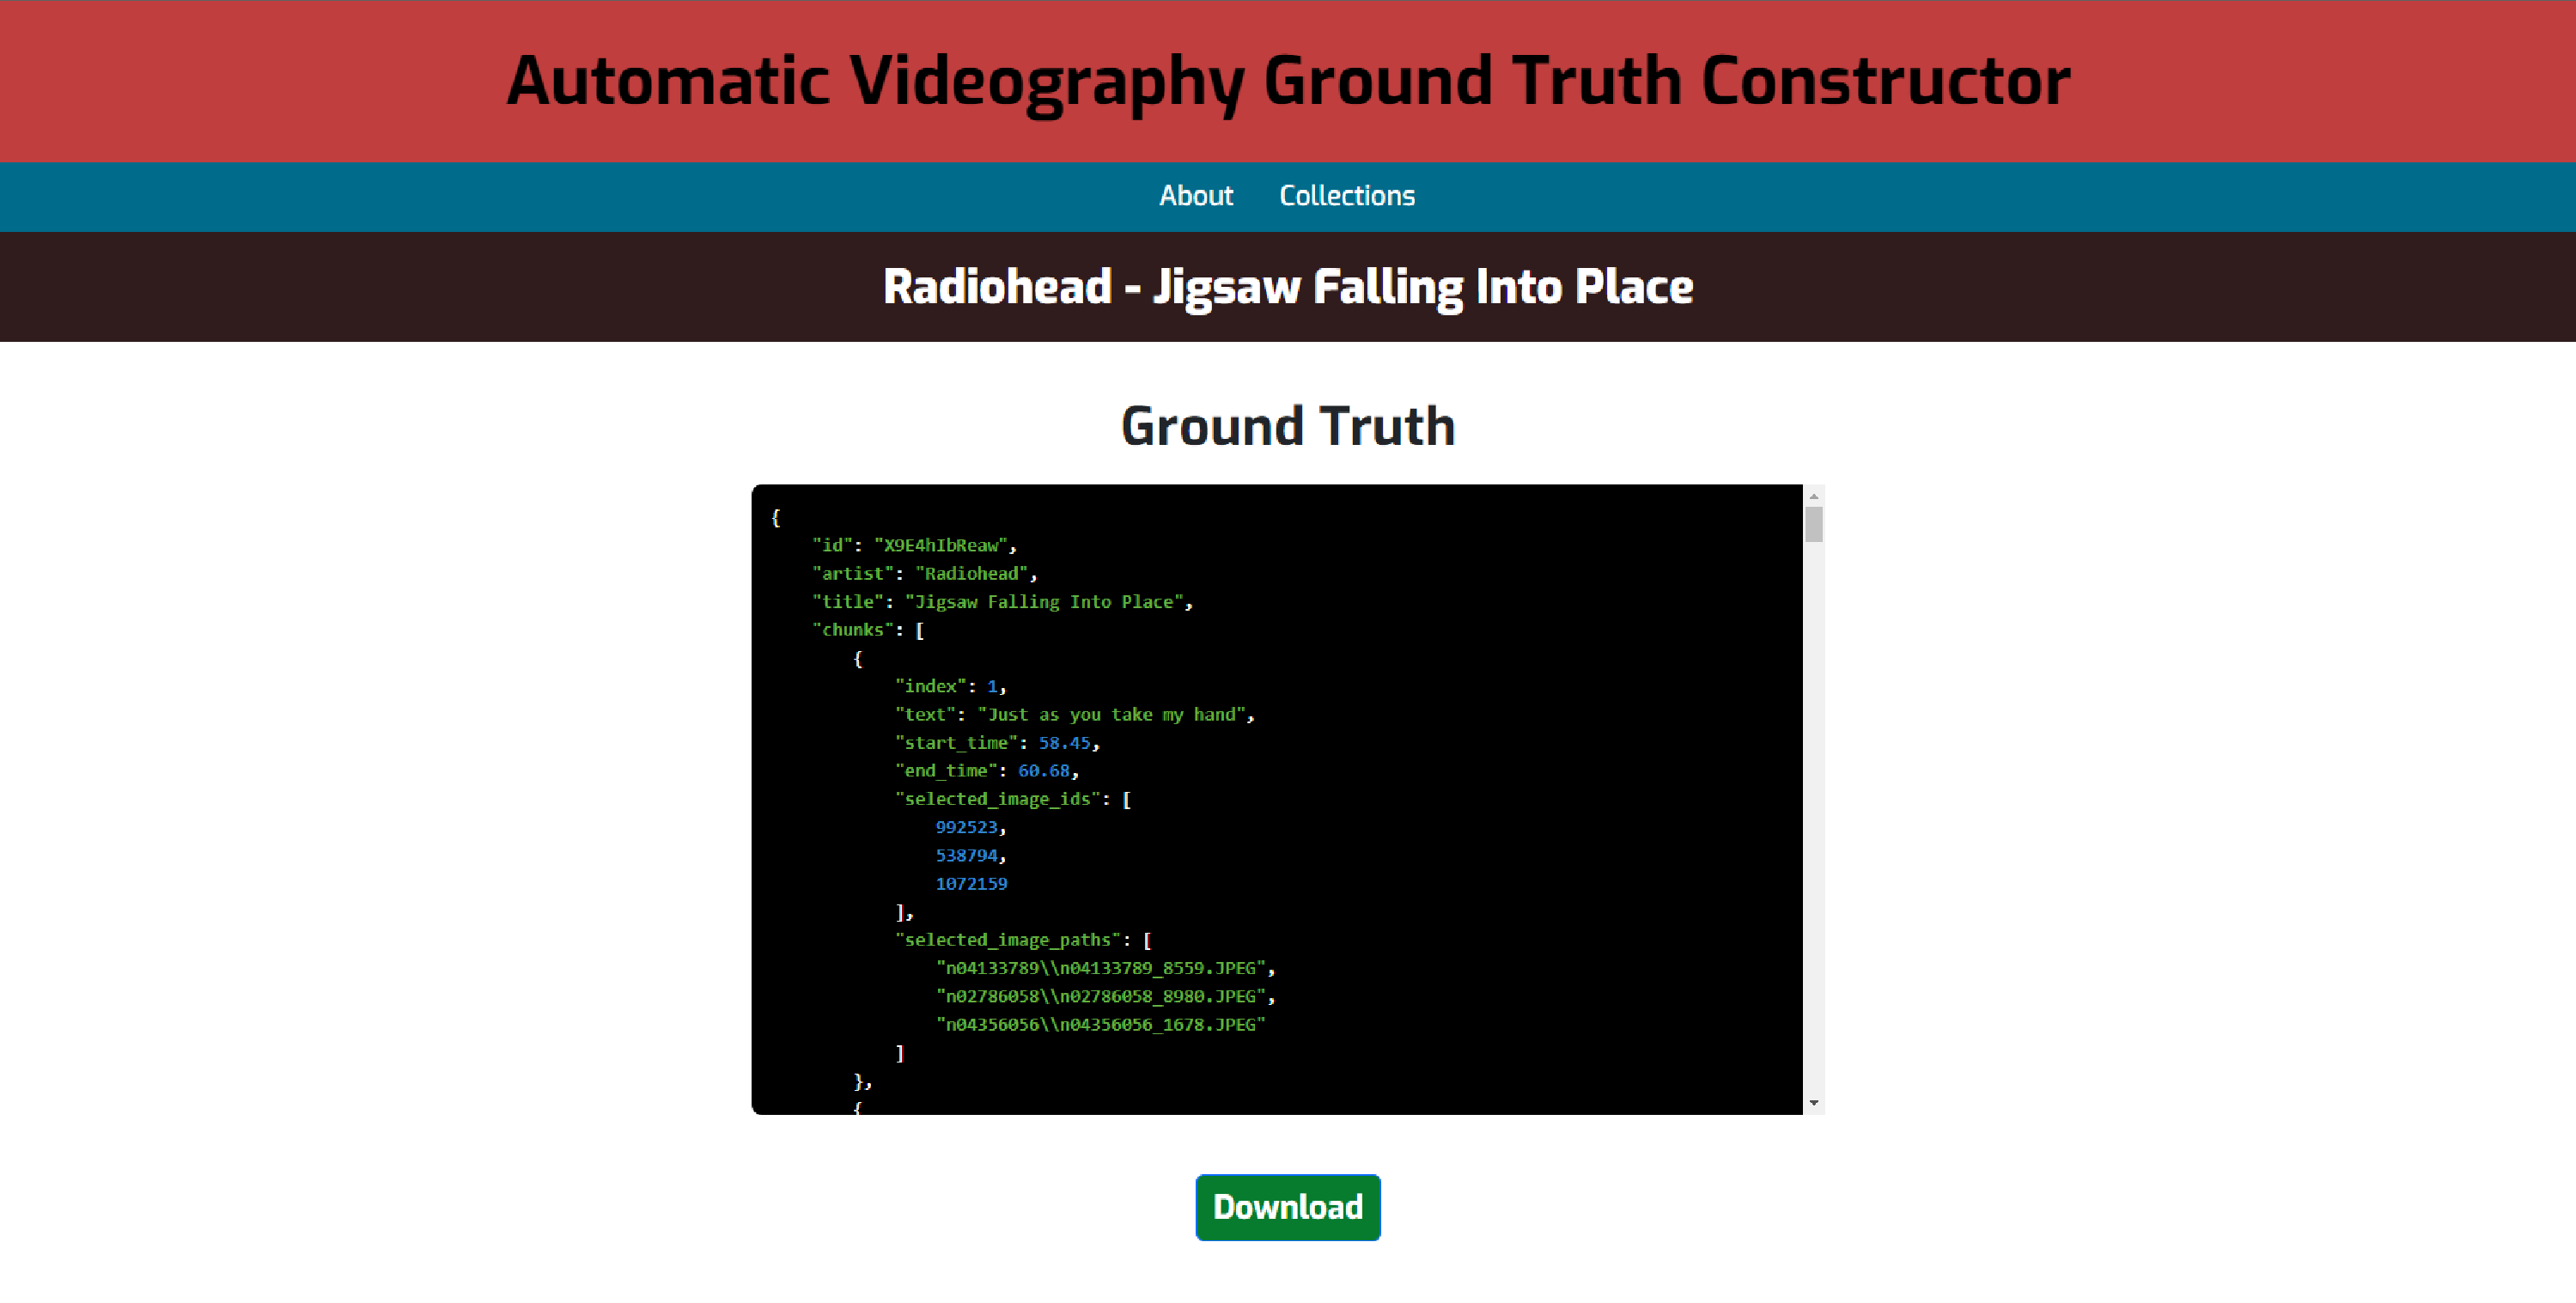
\includegraphics[width=1\textwidth]{figures/walkthrough_ground_truth_page.pdf}
    \caption{Resulting Ground-Truth page after completion for the song "Jigsaw Falling Into Place" by Radiohead}
    \label{fig:walkthrough_ground_truth_page}
\end{figure}

\chapter{Video Generation Time Experiment}
\begin{table}
    \centering
    % \rowcolors{2}{}{gray!3}
    \begin{tabular}{|c|c|c|}
        \hline
        \textbf{Audio Source} & \textbf{Runtime \lstinline|(mm:ss)|} & \textbf{Number of Chunks} \\
        \hline
        \hline
        1 & 04:37 & 61 \\
        \hline
        2 & 02:25 & 42 \\
        \hline
        3 & 02:26 & 62 \\
        \hline
        4 & 03:58 & 81 \\
        \hline
        5 & 04:34 & 80 \\
        \hline
        6 & 04:30 & 62 \\
        \hline
        7 & 02:03 & 34 \\
        \hline
        8 & 03:10 & 36 \\
        \hline
        9 & 04:23 & 53 \\
        \hline
        10 & 03:26 & 69 \\
        \hline
        11 & 04:05 & 74 \\
        \hline
        12 & 03:08 & 51 \\
        \hline
        13 & 04:38 & 36 \\
        \hline
        14 & 04:04 & 21 \\
        \hline
        15 & 03:49 & 37 \\
        \hline
        16 & 03:20 & 38 \\
        \hline
        17 & 02:10 & 26 \\
        \hline
        18 & 04:09 & 43 \\
        \hline
        19 & 03:49 & 26 \\
        \hline
        20 & 04:40 & 26 \\
        \hline
    \end{tabular}
    \caption{Table listing runtime and chunk count information for all 20 audio sources used in the video generation time experiment in \ref{sec:video_generation_time}.}\label{tab:audio_sources}
\end{table}

\begin{table}
    \centering
    \begin{tabular}{|c|c|c|}
        \hline
        \multirow{2}{*}{\textbf{Audio Source}} & 
        \multicolumn{2}{|c|}{\textbf{Video Generation Time \lstinline|(mm:ss)|}} \\
        \cline{2-3} & \textbf{Previous System} & \textbf{New System} \\ 
        \hline
        \hline
        1 & 08:47 & 04:55 \\
        \hline
        2 & 06:55 & 02:30 \\
        \hline
        3 & 09:48 & 03:02 \\
        \hline
        4 & 12:32 & 07:10 \\
        \hline
        5 & 12:24 & 07:36 \\
        \hline
        6 & 09:48 & 06:09 \\
        \hline
        7 & 05:46 & 03:05 \\
        \hline
        8 & 06:03 & 04:43 \\
        \hline
        9 & 08:30 & 06:58 \\
        \hline
        10 & 10:49 & 05:08 \\
        \hline
        11 & 11:32 & 07:12 \\
        \hline
        12 & 08:13 & 04:16 \\
        \hline
        13 & 06:03 & 03:60 \\
        \hline
        14 & 03:54 & 02:48 \\
        \hline
        15 & 06:12 & 02:44 \\
        \hline
        16 & 06:21 & 03:35 \\
        \hline
        17 & 04:37 & 02:33 \\
        \hline
        18 & 07:04 & 04:04 \\
        \hline
        19 & 04:37 & 03:49 \\
        \hline
        20 & 04:37 & 03:15 \\
        \hline
    \end{tabular}
    \caption{Table listing the time from initialising the video generation process and the interface displaying the compiled video for both the preceding and new videography systems. The experiment was run with 20 distinct audio sources which are listed in Table \ref{tab:audio_sources}.}\label{tab:videography_times}
\end{table}


\chapter{Ethics Checklist Form}
\label{app:ethics_checklist}

\includepdf[pages=-]{ethics_checklist.pdf}


\chapter{Usability Evaluation Brief}
\label{app:usability_eval_brief}
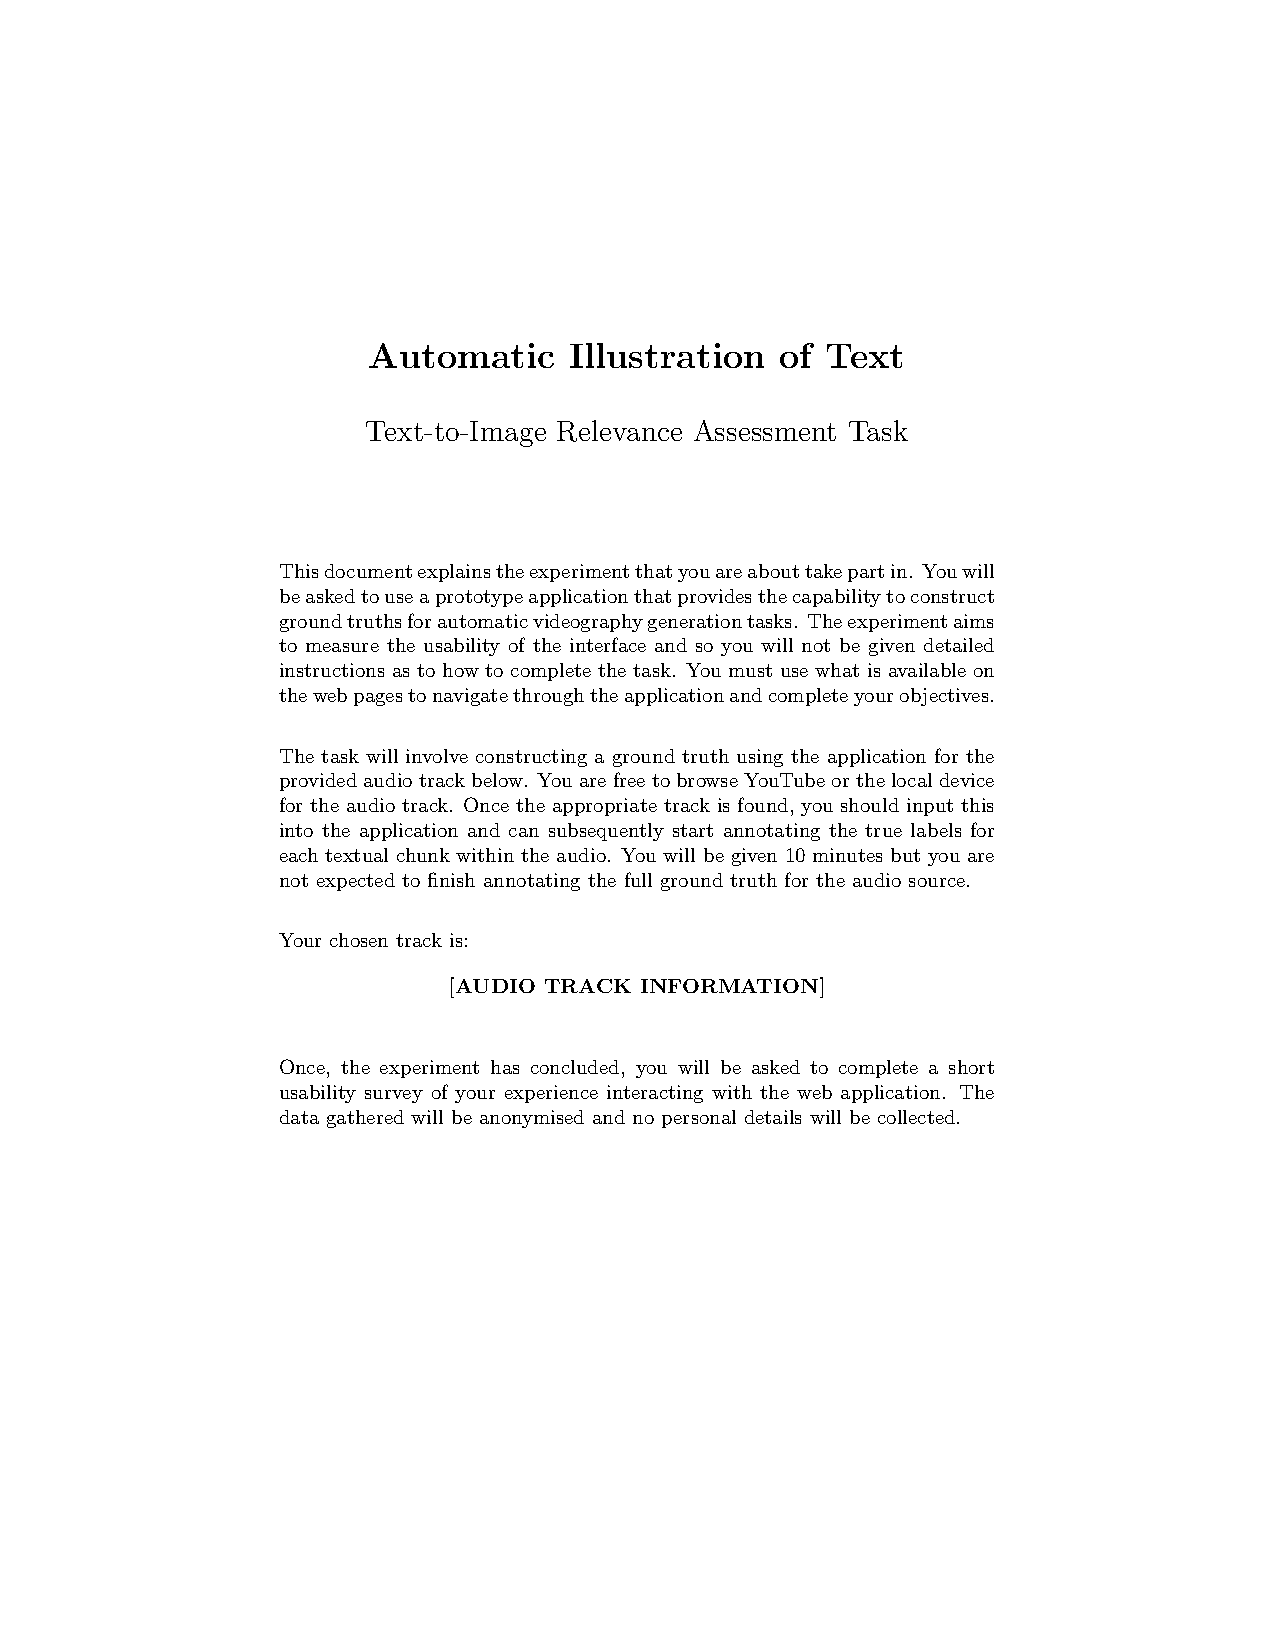
\includepdf[pages=-]{usability_evaluation_task.pdf}


\chapter{Usability Survey Form}
\label{app:usability_survey}
\begin{figure}
    \centering
    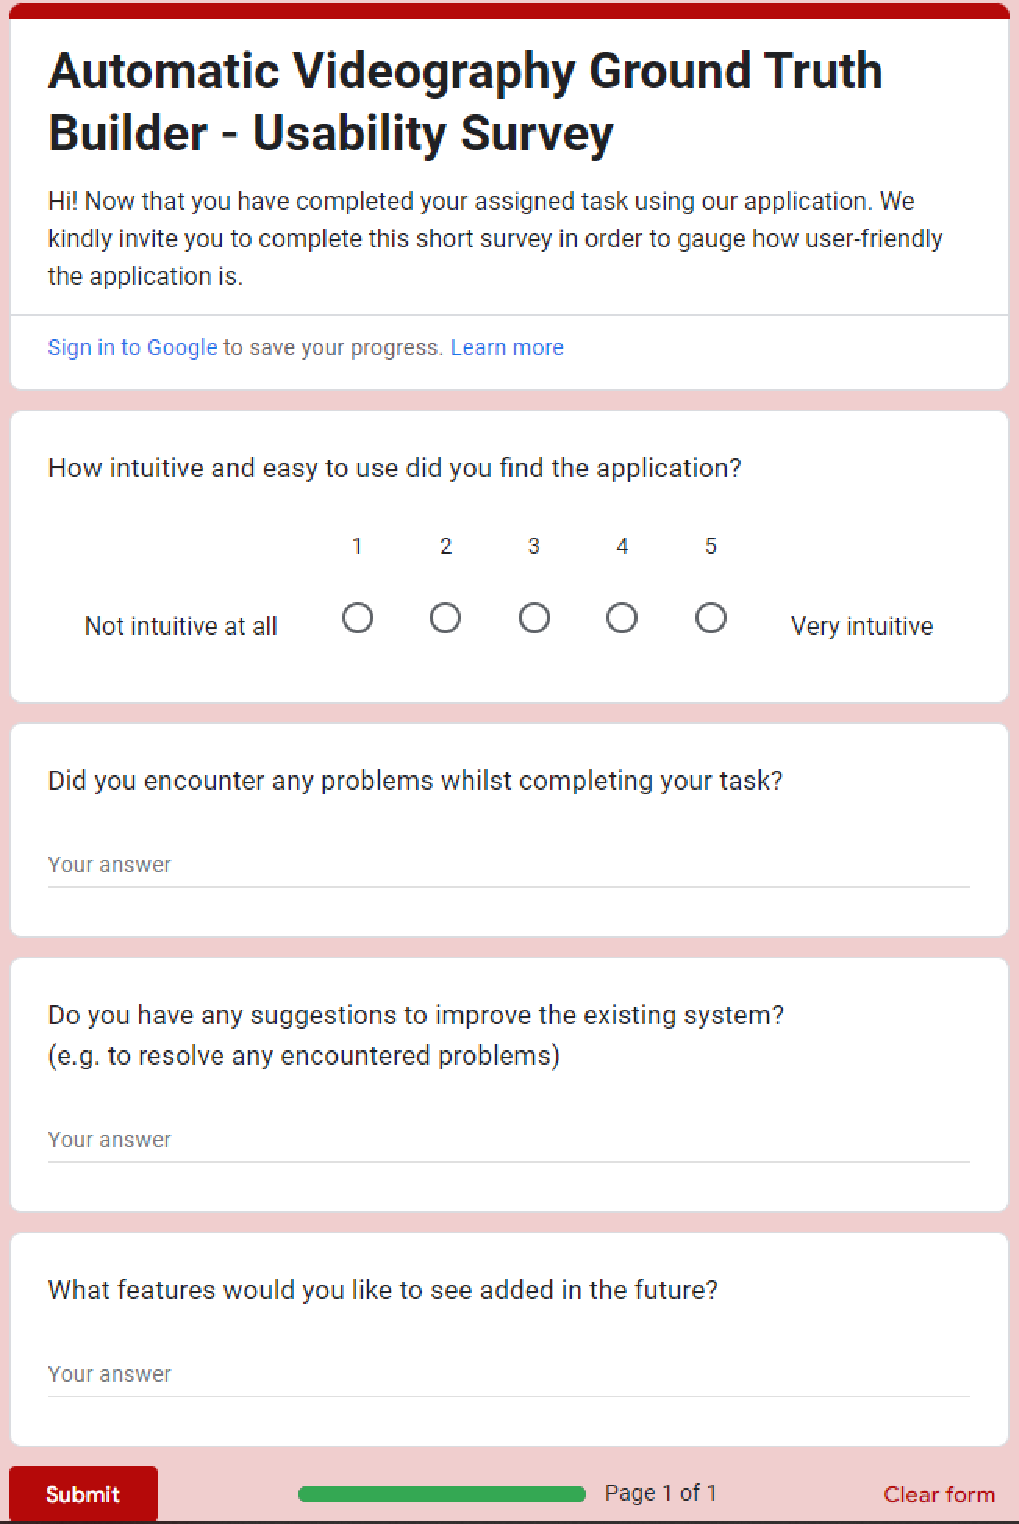
\includegraphics[width=1\textwidth]{figures/usability_survey.pdf}
    \caption{The usability survey form that was given to all sixteen participants after completing their assigned task.}
    \label{fig:usability_survey}
\end{figure}

\end{appendices}
%==================================================================================================
%   BIBLIOGRAPHY   

% The bibliography style is agsm (Harvard)
% The bibliography always appears last, after the appendices.

\bibliographystyle{agsm}

% Force the bibliography not to be numbered
\renewcommand{\thechapter}{0} 
\bibliography{l4proj}

\end{document}
